\chapter{Signal Reconstruction Techniques for Antenna Array CRES and the FSCD}

\section{Introduction}

The transition from a waveguide CRES experiment to an antenna array CRES experiment introduces new challenges related to data acquisition, signal detection, and signal reconstruction caused by the multi-channel nature of the data. The development of signal reconstruction algorithms is crucial to the design of antenna array based experiments like the FSCD, because these algorithms directly influence the detection efficiency and energy resolution of the CRES experiment. In this Chapter I summarize my contributions to the development and analysis of signal reconstruction and detection algorithms for the FSCD experiment.

In Section \ref{sec:chap4-simulations} I discuss the primary tool for this work, which is the Locust simulations package developed by the Project 8 experiment. Locust is used to simulate CRES events in the detector. Locust uses Kassiopeia to calculate particle trajectory solutions for electrons in the magnetic trap. The trajectories are then used to calculate the response of the antenna array to the cyclotron radiation produced by the electron, which results in signals that can be used to analyze the performance of different signal reconstruction algorithms. More recently, Project 8 has developed CREsana, which is a new simulations package that takes a more analytical approach to CRES signal simulations for antenna arrays. Although CRESana signals were not used for the signal reconstruction algorithm development detailed here, we introduce the software as it plays a role in the antenna array measurements presented in Section \ref{sec:chap5-fscd-array-measurements}.

In Section \ref{sec:chap4-pter} I discuss the signal reconstruction and detection approaches analyzed for the FSCD experiment. In general there are two steps to signal reconstruction --- detection and parameter estimation. With signal detection one is primarily concerned only with distinguishing between data that contains a signal versus data that contains only noise, whereas, with parameter estimation one is interested in extracting the kinematic parameters of the electron encoded in the cyclotron radiation signal shape. Due to the low signal power of electrons near the spectrum endpoint in the FSCD experiment, signal detection is a non-trivial problem. This is magnified by the need to maximize the detection efficiency of the experiment in order to achieve the neutrino mass sensitivity goals. My contributions to signal reconstruction analysis fof the FSCD are focused on this signal detection component of reconstruction.

After the discussion of various signal detection approaches, in Section \ref{sec:chap4-trigger-paper} I present a more detailed analysis of the detection performance of three algorithms, which could be used to signal detection in the FSCD. This section was originally prepared for publication in JINST as a separate paper. The algorithms include a digital beamforming algorithm, a matched filter algorithm, and a neural network algorithm, which I analyze in terms of classification accuracy and estimated computational cost.  

\section{FSCD Simulations}
\label{sec:chap4-simulations}

Antenna array CRES and the FSCD requires a combination of different capabilities not often found in a single simulation tool. First of all, accurate calculations of the magneto-static fields produced by current-carrying coils are required in order to accurately model the magnetic trap and background magnets. The resulting magnetic fields must then be used to calculate the exact relativistic trajectory of electrons, which is required in order to calculate the electro-magnetic (EM) fields produced by the acceleration of the electron. Finally, the simulation has to model the interaction of the antenna and RF receiver chain with these EM-fields in order to produce the simulated voltage signals produced by the antenna array during the CRES event. At the time when Project 8 was developing this simulation capability, no single available simulation tool was known to adequately perform this suite of calculations, which prompted the development of custom simulation framework to simulate the FSCD. This simulation framework includes custom simulation tools developed by Project 8 as well as other open-source and proprietary software developed by third-parties.

\subsection{Kassiopeia}

Kassiopeia\footnote{https://github.com/KATRIN-Experiment/Kassiopeia} is a particle tracking and static EM-field solver developed by the KATRIN collaboration for simulations of their spectrometer based on magnetic adiabatic collimation with an electrostatic filter \cite{kassiopeia}. Due to the measurement technique employed by the KATRIN collaboration, Kassiopeia is not designed to solve for the EM-fields produced by electrons in magnetic fields. However, it does provide efficient solvers for static electric and magnetic fields and charged particle trajectory solvers. Because of this, Project 8 has incorporated parts of Kassiopeia into it's own simulation framework. 

\subsubsection*{Magnetostatic Field Solutions}

The solutions to the electric and magnetic fields generated by a static configuration of charges and currents is given by Maxwell's equations in the limit where the time-dependent terms go to zero. In their static form Maxwell's equations \cite{jackson_classical_1999} are
\begin{align}
    \nabla\cdot\mathbf{E}&=\frac{\rho}{\epsilon_0}\\
    \nabla\times\mathbf{E}&=0\\
    \nabla\cdot\mathbf{B}&=0\\
    \nabla\times\mathbf{B}&=\mu_0\mathbf{J},
\end{align}
where we can see that the electric and magnetic fields are now completely decoupled from each other. The solution for the magnetic field in this boundary value problem is given by the Biot-Savart law
\begin{equation}
    \mathbf{B}(\mathbf{r}) = \frac{\mu_0}{4\pi}\int_{}^{}{d{r^{'}}^{3}\frac{\mathbf{J}(\mathbf{r}^{'})\times (\mathbf{r}-\mathbf{r}^{'})}{|\mathbf{r}^{'}-\mathbf{r}|^{3}}},
\end{equation}
which Kassiopeia uses a variety of numeric integration techniques to solve for a user defined current distribution.

\subsubsection*{Kassiopeia Simulation of the FSCD Magnetic Trap}

The trap developed for the FSCD experiment utilizes six current carrying coils, which surround a cylindrical tritium containment vessel (see Figure \ref{fig:chap4-trap10-coils}). Some critical aspects of the trap design include the total trapping volume, the maximum trap depth, the steepness of the trap walls, as well as the radial and azimuthal uniformity of the magnetic fields.

The volume of the FSCD trap is a cylindrically shaped region with a radius of 5~cm and a length of 15~cm resulting in a roughly 1~L total trap volume. The trap volume is an important design feature, because it sets the volume of the experiment that is potentially usable for CRES measurements. Trapping a larger volume allows one to observe a larger number of tritium atoms, which increases the statistical power and sensitivity of the neutrino mass measurement. Due to the cost of constructing magnets with large and uniform magnetic fields it is important that the trap use as much of the available volume as possible to limit the overall cost of the experiment.

\begin{table}[htbp]
    \footnotesize
    \begin{minipage}{0.65\textwidth}
        \centering
        \begin{tabular}{c|c|c|c}
            Coil & Radius (mm) & Z Pos. (mm) & Current (A$\times$Turns)\\
            \hline
            1 & 50.0 & -92.3 & 750.0\\
            2 & 50.1 & -56.9 & -220.3\\
            3 & 68.5 & -19.5 & -250.0\\
            4 & 68.5 & 19.5 & -250.0\\
            5 & 50.1 & 56.9 & -220.3\\
            6 & 50.0 & 92.3 & 750.0\\
        \end{tabular}
        \end{minipage}
    \begin{minipage}{0.35\textwidth}
        \centering
        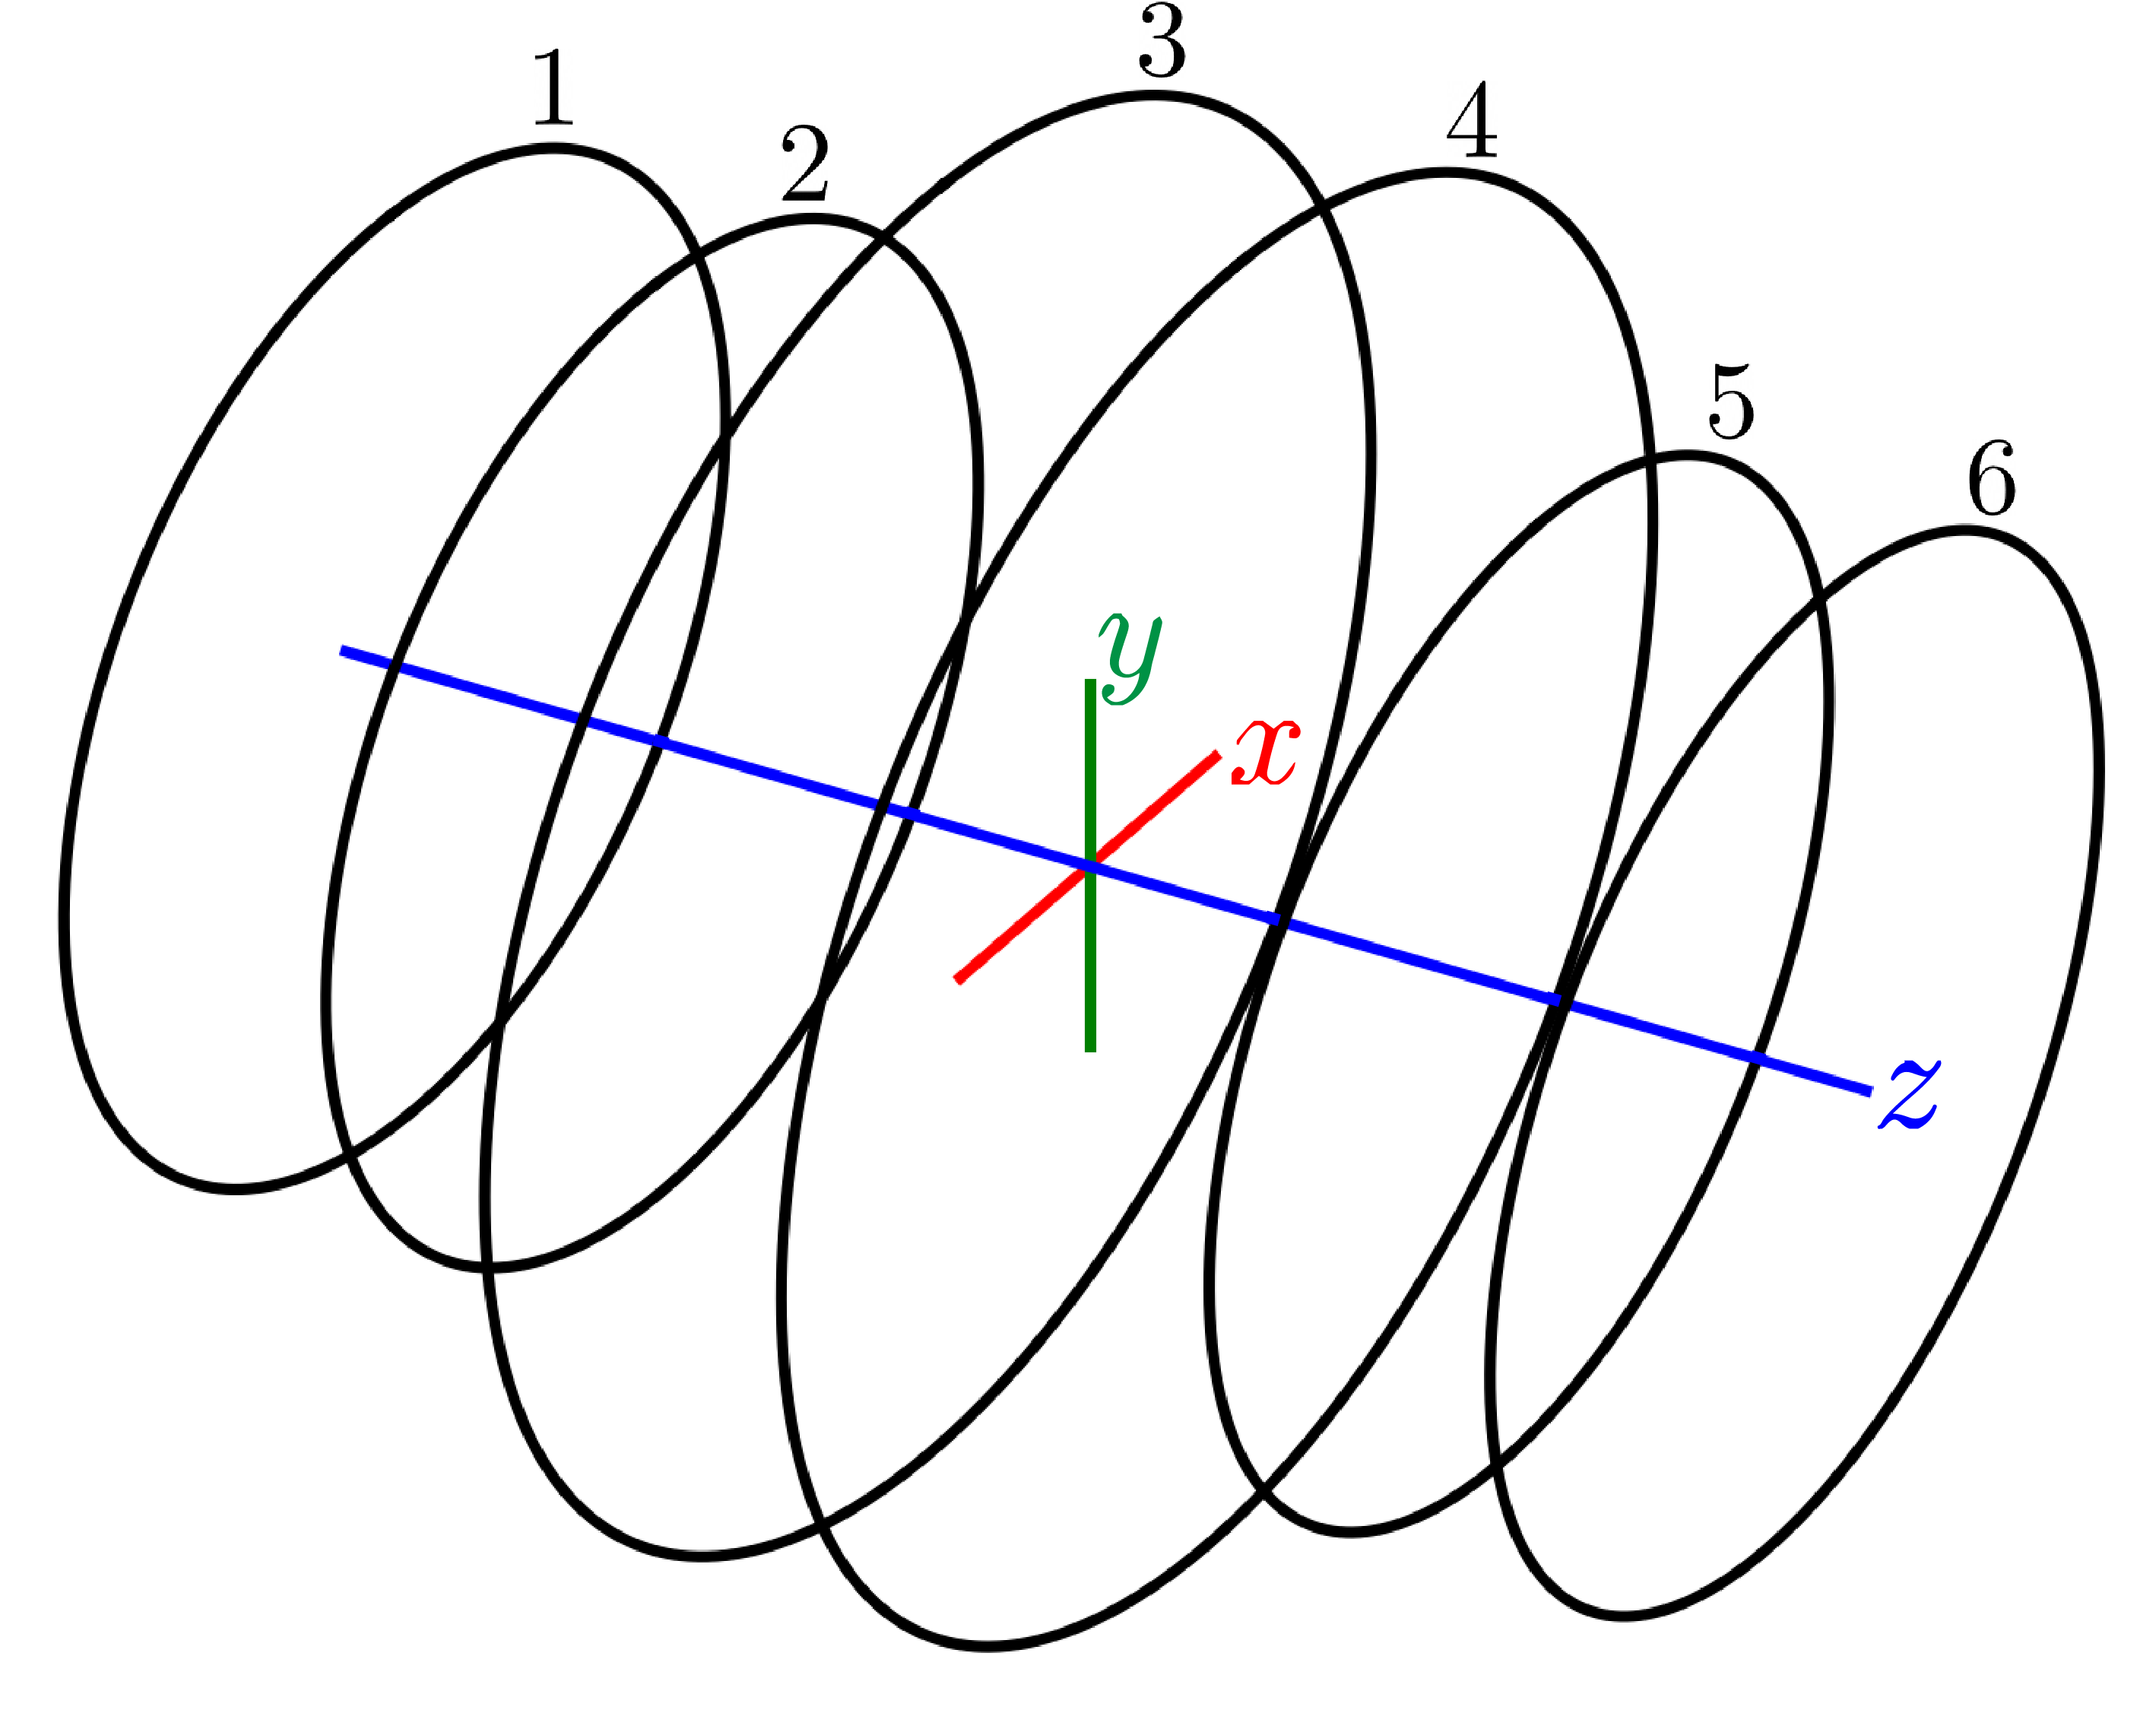
\includegraphics[width=1\textwidth]{figs/Chapter-4/230512_trap10_coils.png}
        \label{fig:chap4-trap10-coils} 
    \end{minipage}
    \par
    \centering
    \begin{minipage}{0.7\textwidth}
        \centering
        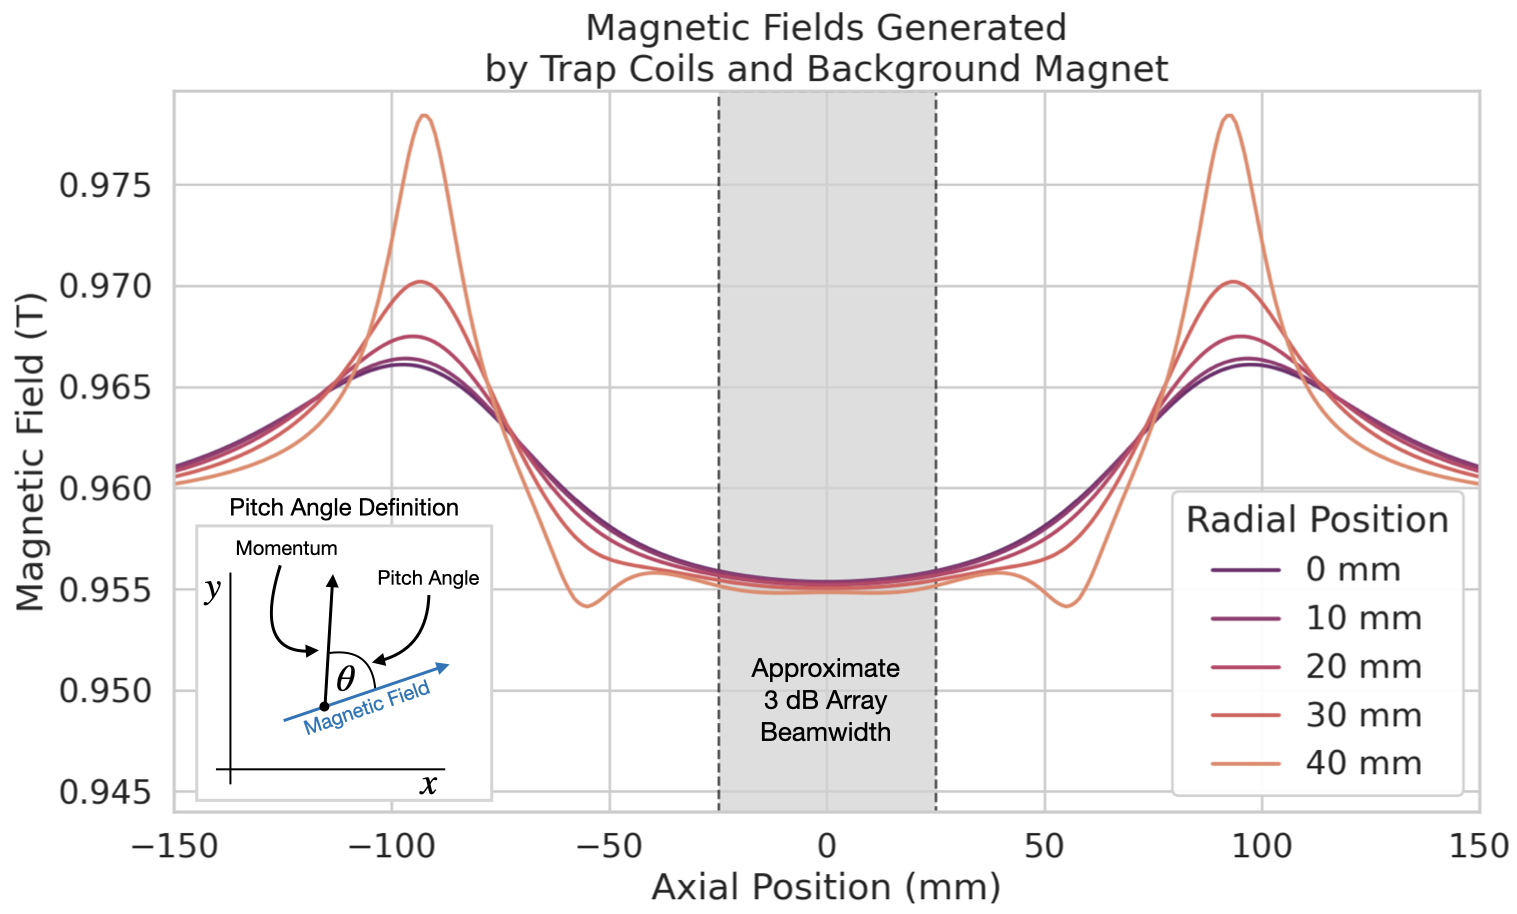
\includegraphics[width=1\textwidth]{figs/Chapter-4/230214_annotate_trap_profile_image.001.png}
    \end{minipage}
    \captionof{figure}{The geometry and parameters of the coils used to simulate the FSCD magnetic trap in Kassiopeia. Some axial profiles of the magnetic trap at different radial positions are show to demonstrate the shape of the magnetic field and trap depth as a function of position. Calulation of the magnetic field profiles was graciously done by Ren\'{e} Reimann.}
    \label{fig:chap4-trap10-coils}
\end{table}

The depth of the FSCD trap is approximately 10~mT when measured along the central axis, which is sufficient to trap electrons with pitch angles as small as $84^\circ$. The trap depth factors into the efficiency of the experiment by directly controlling the range of electron pitch angles that can be trapped. If a higher fraction of pitch angles are trapped then, in principle, more decay events can be observed. However, the signals from electrons with small pitch angles are typically significantly harder to detect than larger pitch angles when using an antenna array, which increases the likelihood of not detecting the first track of the CRES event and harms the energy resolution of the experiment. 

The steepness of the trap walls as well as any non-uniformities in the magnetic field contribute to the total energy resolution of the CRES measurement by causing uncertainty in the relationship between an electron's kinetic energy and it's cyclotron frequency. When an electron is trapped, it oscillates back and forth along the trap z-axis (see Figure \ref{fig:chap4-trap10-coils}) unless it is produced with a pitch angle of exactly $90^\circ$ \cite{p8pheno}. As the electron is reflected from the trap walls it experiences a change in the total magnetic field, which causes a modulation in the cyclotron frequency. This change in magnetic field from the trap introduces a correlation between the pitch angle and kinetic energy parameters of the electron that can reduce energy resolution. In order to mitigate this effect it is important to make the trap walls as steep as possible. 

%\begin{figure}[htbp]
%    \centering
%    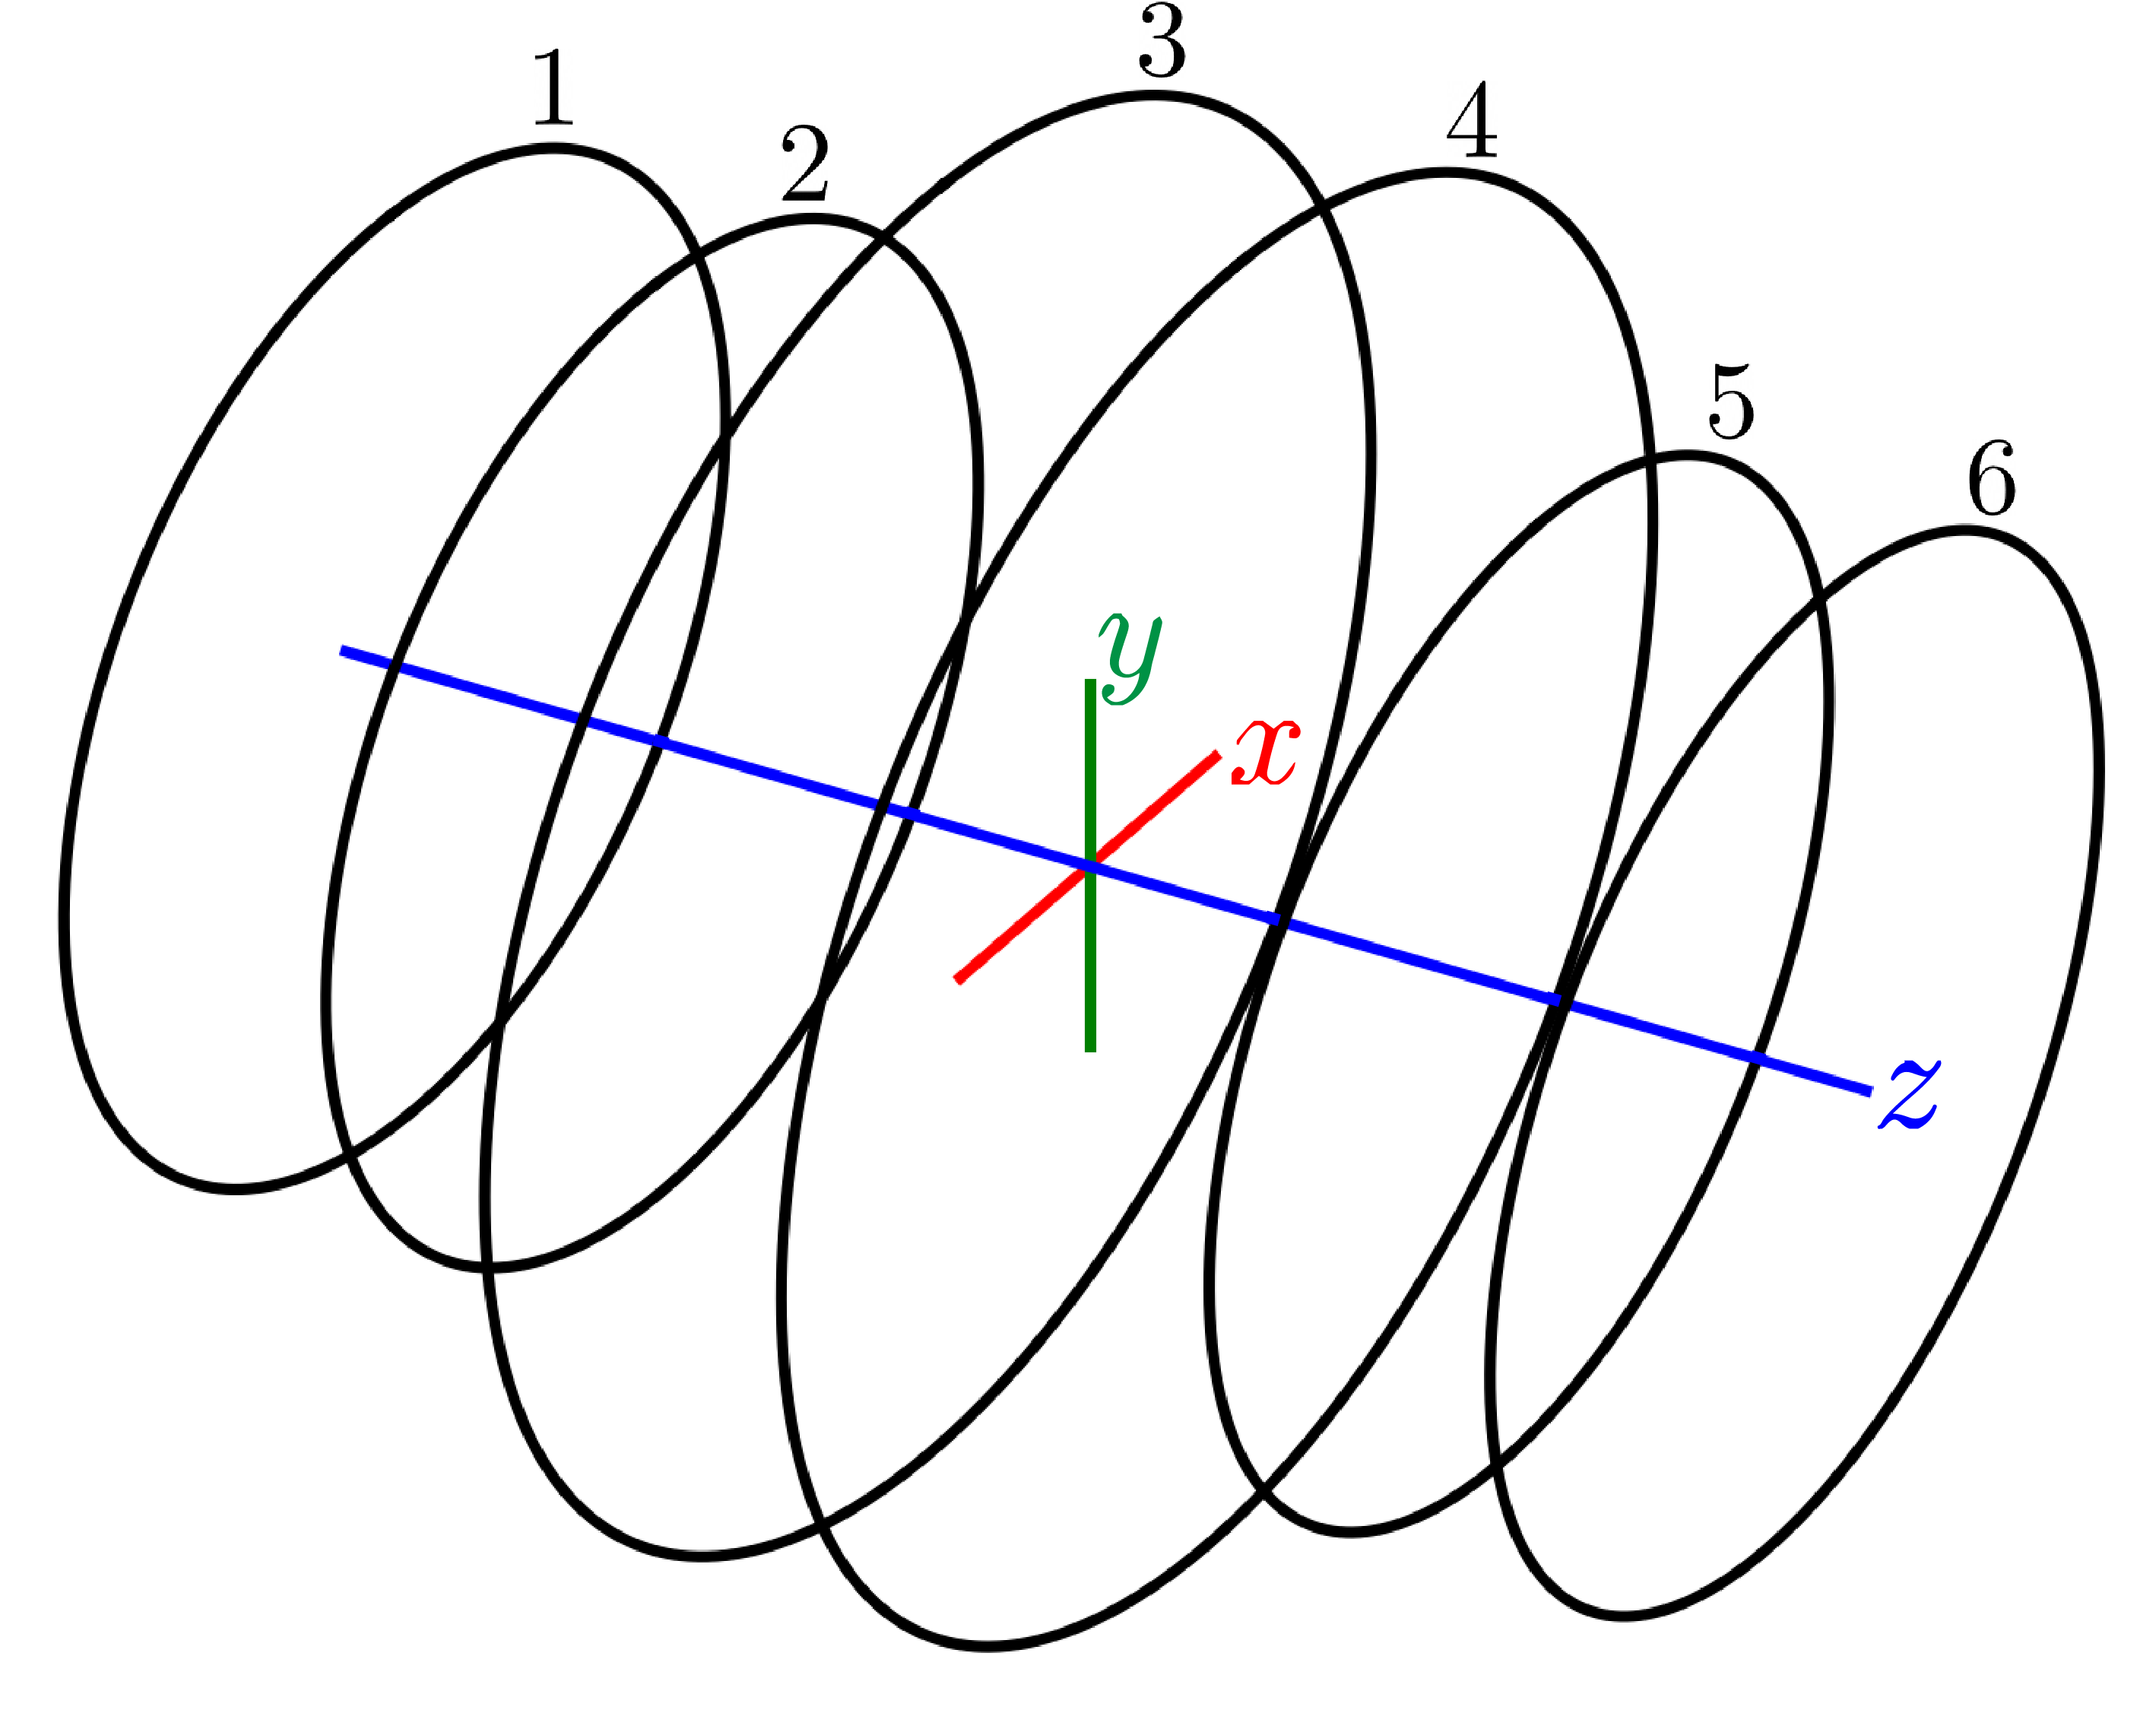
\includegraphics[width=0.5\textwidth]{figs/Chapter-4/230512_trap10_coils.png}
%    \caption{Caption}
%    \label{fig:chap4-trap10-coils}
%\end{figure}


%\begin{figure}[htbp]
%    \centering
%    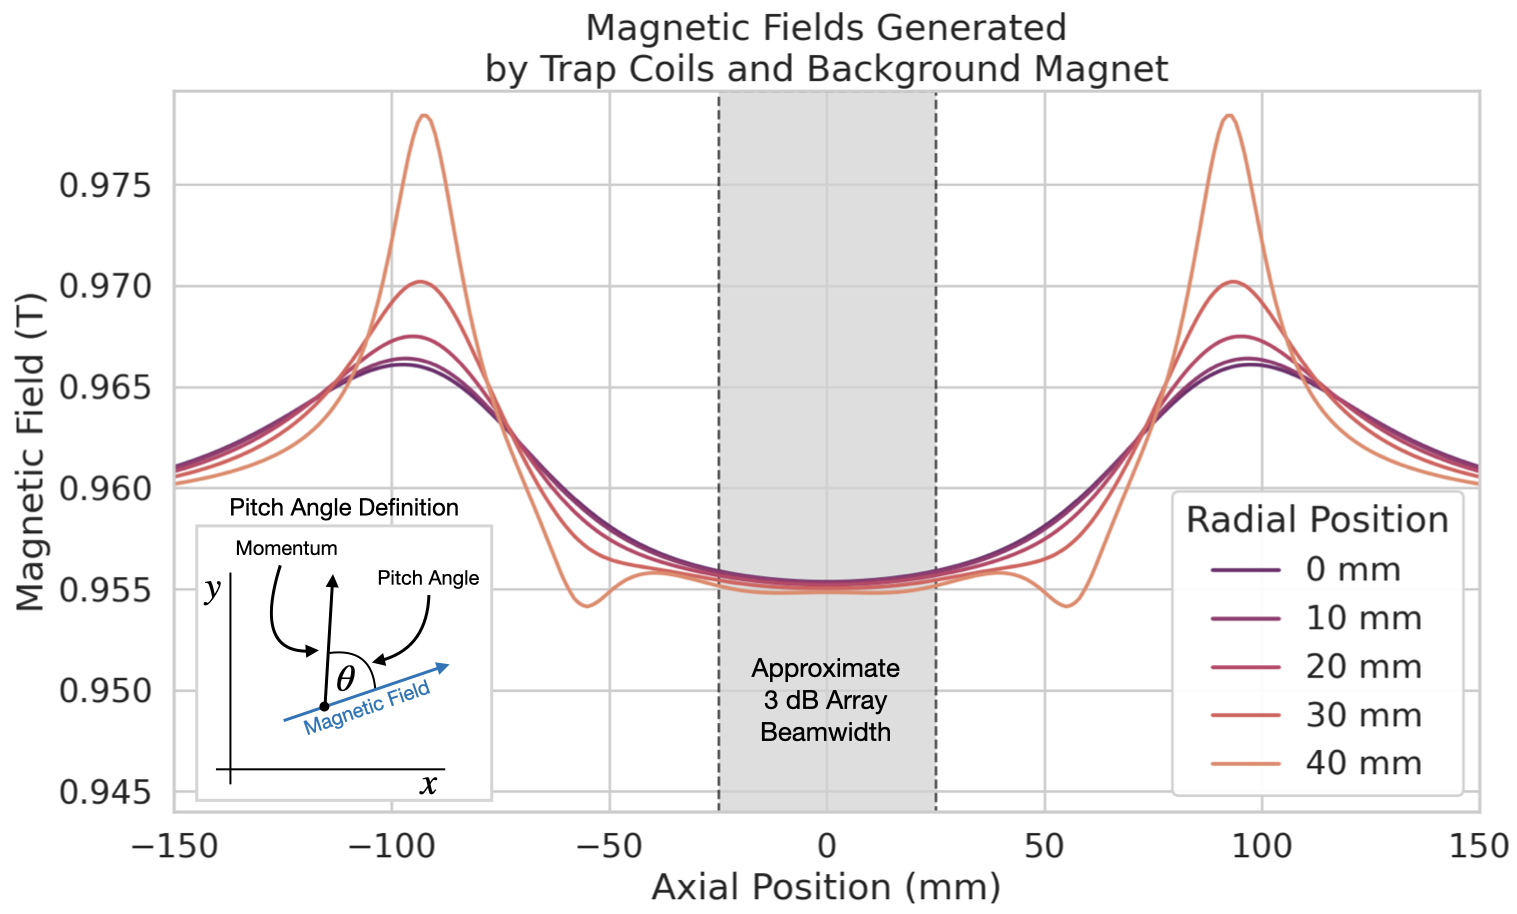
\includegraphics[width=0.7\textwidth]{figs/Chapter-4/230214_annotate_trap_profile_image.001.png}
%    \caption{Profiles of the magnetic fields produced by a prototype magnetic trap and background magnet designed for the FSCD experiment.}
%    \label{fig:chap4-mag-trap-profile}
%\end{figure}

\subsubsection*{Particle Trajectory Solutions}

The magnetic fields solved by direct integration of the electron's current density can be used by Kassiopeia to solve for the trajectory of electrons based on user specified initial conditions. Various distributions are available within Kassiopeia that can be sampled in order to replicate realistic event statistics, including uniform, Gaussian, and Lorentzian among others. In general, an electron has six kinematic parameters that define its trajectory, which are the three-dimensional coordinates of the initial position and the three components of the electron's momentum vector. However, when simulating CRES events it is more common to parameterize the electron's trajectory in terms of it's initial position, the kinetic energy, the pitch angle, and the initial direction of the component of the electron's momentum perpendicular to the magnetic field. This parameterization is completely equivalent to specify each component of the electrons initial position and momentum vectors. 

From the initial parameters of the electron and the magnetic field, Kassiopeia solves for the trajectory of the electron. The direct approach proceeds by solving the motion of the electron using the Lorentz force equation, which takes the form of a set of differential equations 
\begin{align}
    \frac{d\mathbf{r}}{dt}&=\frac{\mathbf{p}}{\gamma m}\\
    \frac{d\mathbf{p}}{dt}&=e(\mathbf{E}+\frac{\mathbf{p}\times\mathbf{B}}{\gamma m}),
\end{align}
where $\mathbf{r}$ is the position of the electron, $\mathbf{p}$ is the electron's momentum, $e$ is the charge of the electron, $m$ is the electron's mass, and $\gamma$ is the relativistic Lorentz term. To account for kinetic energy losses from radiation Kassiopeia includes an additional term in the momentum differential equation, which calculates the change in the electron's momentum induced by synchrotron radiation. Kassiopeia solves this pair of differential equations using numerical integration, however, the exact trajectory can be computationally intensive to solve. If the adiabatic approximation can be applied, then Kassiopeia can make use of a simpler set of equations that can be more readily solved numerically. 

\begin{figure}[htbp]
    \centering
    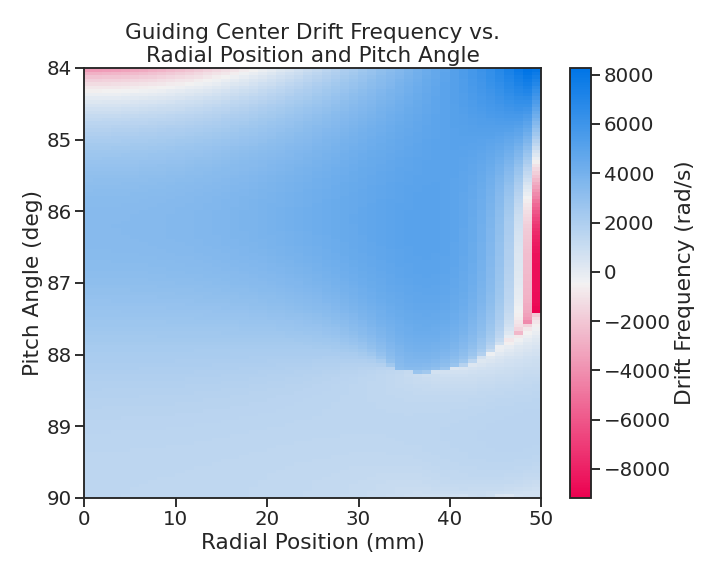
\includegraphics[width=0.6\textwidth]{figs/Chapter-4/230220_gradb_drift_frequencies.png}
    \caption{A map of the average $\nabla B$-drift frequency for electrons trapped in the prototype FSCD trap shown in Figure \ref{fig:chap4-trap10-coils}. Negative drift frequencies indicate electrons that are drifting opposite to the standard direction, which means that they are close to escaping the magnetic trap.}
    \label{fig:chap4-gradb-drift-frequency-map}
\end{figure}

Even though Kassiopeia is not directly capable of simulating the cyclotron radiation, it is still an invaluable CRES simulation tool, due to the accurate trajectory solutions for electrons in magnetic traps. With Kassiopeia it is possible to test the efficiency of a particular trap design and analyze features of the electron trajectories that are important to the position, track, and event reconstruction algorithms (see Section \ref{sec:chap4-pter}). One example of this for the FSCD is the analysis of the average $\nabla B$-drift frequency as a function of the electrons radial position and pitch angle in the magnetic trap (see Figure \ref{fig:chap4-gradb-drift-frequency-map}). Radial gradients in the trap cause the guiding center of the electron to drift around the center of the magnetic trap with an average frequency on the order of $10^3$~rad/s. This frequency, while slow compared to the length of a typical CRES time-slice, is large enough to cause a significant loss in efficiency of certain signal reconstruction algorithms. Therefore, it is important to model the drift of the electron in the reconstruction algorithm in order to mitigate the effects of this motion on the reconstruction.

\subsection{Locust}

The Locust\footnote{\url{https://github.com/project8/locust_mc/tree/master}} software package \cite{p8locustpaper} is the primary simulation tool developed and used by the Project 8 collaboration for CRES experiments. Locust simulates the responses of antennas and receiver electronics chain to rapidly time-varying electric fields using a flexible approach that allows one to choose from a variety of electric field sources and antennas. Similarly, one can simulate the receiver chain using a series of modular generators that include standard signal processing operations such as down-mixing and fast Fourier transforms (FFT). Since the primary focus of this chapter is the application of Locust to analyses of the FSCD, we shall describe only the most relevant aspects of the software rather than provide a comprehensive description.

\subsubsection*{Cyclotron Radiation Field Solutions}

Simulating CRES events in the FSCD requires that we calculate the electric fields produced by the acceleration of the electron. In the general case, this can be a complicated question to answer, due to back-reaction forces on the electron from it's own electric fields that occur when the electron is surrounded by conductive material such as a waveguide or cavity. However, in the case of the FSCD it is possible to ignore such effects and approximate the electron as radiating into a free-space environment. 

The equations that describe the electromagnetic fields from a relativistic moving point particle are the Li\'{e}nard-Wiechert field equations \cite{lw_potential_1,lw_potential_2}, which are obtained by differentiating the Li\'{e}nard-Wiechert potentials. In their full form the Li\'{e}nard-Wiechert field equations are
\begin{align}
    \bm{E} &=e\left[\frac{\hat{n}-\bm{\beta}}{\gamma^2(1-\bm{\beta}\cdot\hat{n})^3|\bm{R}|^2}\right]_{t_\textrm{r}}
      +\frac{e}{c}\left[\frac{\hat{n}\times[(\hat{n}-\bm{\beta})\times\dot{\bm{\beta}}]}{(1-\bm{\beta}\cdot\hat{n})^3|\bm{R}|}\right]_{t_\textrm{r}}\label{eq:chap4-lw-eqn-efield}\\
    \bm{B} &= \left[\hat{n}\times \bm{E}\right]_{t_\textrm{r}},
\end{align}
where $e$ is the charge of the particle, $\hat{n}$ is the unit vector pointing from the particle to the position where the fields are calculated, $\bm{\beta}$ and $\dot{\bm{\beta}}$ are the velocity and acceleration of the particle divided by the speed of light ($c$), $\bm{R}$ is the distance from the particle to the field calculation position, and $\gamma$ is the relativistic Lorentz term. The subscript $t_\mathrm{r}$ indicates that the equations must be evaluated at the retarded time so that the time-delay from the travel time of the electromagnetic radiation is correctly accounted for. 

The only required input to calculate the electric field at the position of an FSCD antenna is the velocity and acceleration of the electron, which can be obtained from Kassiopeia simulations. Therefore, when simulating a CRES event Locust first runs a Kassiopeia simulation of the electron and calculates the electric field incident on the antenna. The only difficulty with this approach is the determination of the retarded time. The retarded time corresponds to the time that a photon, which has just arrived at an antenna at the space-time position $(t,\bm{r})$, was actually emitted by the electron at the space-time position of $(t_\mathrm{r}, \bm{r}_e(t_\mathrm{r}))$. Defined in this way, finding the retarded time requires solving 
\begin{equation}
    c(t-t_\mathrm{r}) = |\bm{r}-\bm{r}_e(t_\mathrm{r})|,
    \label{eq:chap4-ret-time-condition}
\end{equation}
where the distance traveled by the photon between the measurement and retarded times is equal to the distance between the antenna and the electron at the retarded time. Locust solves Equation \ref{eq:chap4-ret-time-condition} using a built-in root finding algorithm to find the retarded time, and thus the electric field produced by the electron at the position of each antenna in the FSCD array.

\subsubsection*{Antenna Response Modeling}

With the electric field it is possible, in principle, to calculate the resulting voltages produced in the antenna. However, direct simulation of the antenna itself is computationally expensive since it would require the modeling of complex interactions of the electron's electric fields with charge carriers in the conductive elements of the antenna. Direct simulation of the antenna in Locust can be avoided by modeling the antenna response using the antenna factor, or antenna transfer function, approach. The antenna factor defines the voltage produced in the antenna terminal for an incident electric field \cite{balanis2015antenna},
\begin{equation}
    A_\mathrm{F}=\frac{V}{|\bm{E}|},
\end{equation}
where V is the voltage and $|\bm{E}|$ is the magnitude of the incident electric field. To obtain the antenna factor for the antennas developed for the FSCD Project 8 employs Ansys HFSS. HFSS is a commercially available finite element method electromagnetic solver widely used throughout the antenna engineering industry \cite{hfss}. HFSS is capable of calculating the antenna factor and gain patterns for complex antenna designs and outputting the resulting quantities in the form of a text file that can be used as an input to the Locust simulation. 

The antenna factor defines the steady-state response of the antenna to electromagnetic plane waves and is a function of the frequency of the radiation. Therefore, in order to apply the transfer function for the calculation of the antenna voltage response in the time domain, Locust models the antenna as a linear time-invariant system \cite{lti_theory_wiki}. In this formalism the response of the system to the driving force is given by 
\begin{equation}
    y[n] = h\ast x=\sum_{k}{h[k]x[n-k]},
\end{equation}
where $y[n]$ is the discretely sampled response, $x$ is the driving force stimulus, and $h$ is the finite impulse response (FIR) filter. When applied to the FSCD array, this formalism calculates the voltage time-series produced in each antenna by convolving the electric field time-series with the antenna FIR filter, which is obtained by performing a inverse Fourier transform on the transfer function from HFSS. 

\subsubsection*{Radio-frequency Receiver and Signal Processing}

After obtaining the voltage time-series by computing the electron trajectory and antenna response, Locust simulates the signal processing associated with the radio-frequency receiver chain. The standard receiver chain used in Locust simulations of the FSCD attempts to mimic the operations that would actually occur in hardware (see Figure \ref{fig:chap4-locust-receiver-chain}). 

\begin{figure}[htbp]
    \centering
    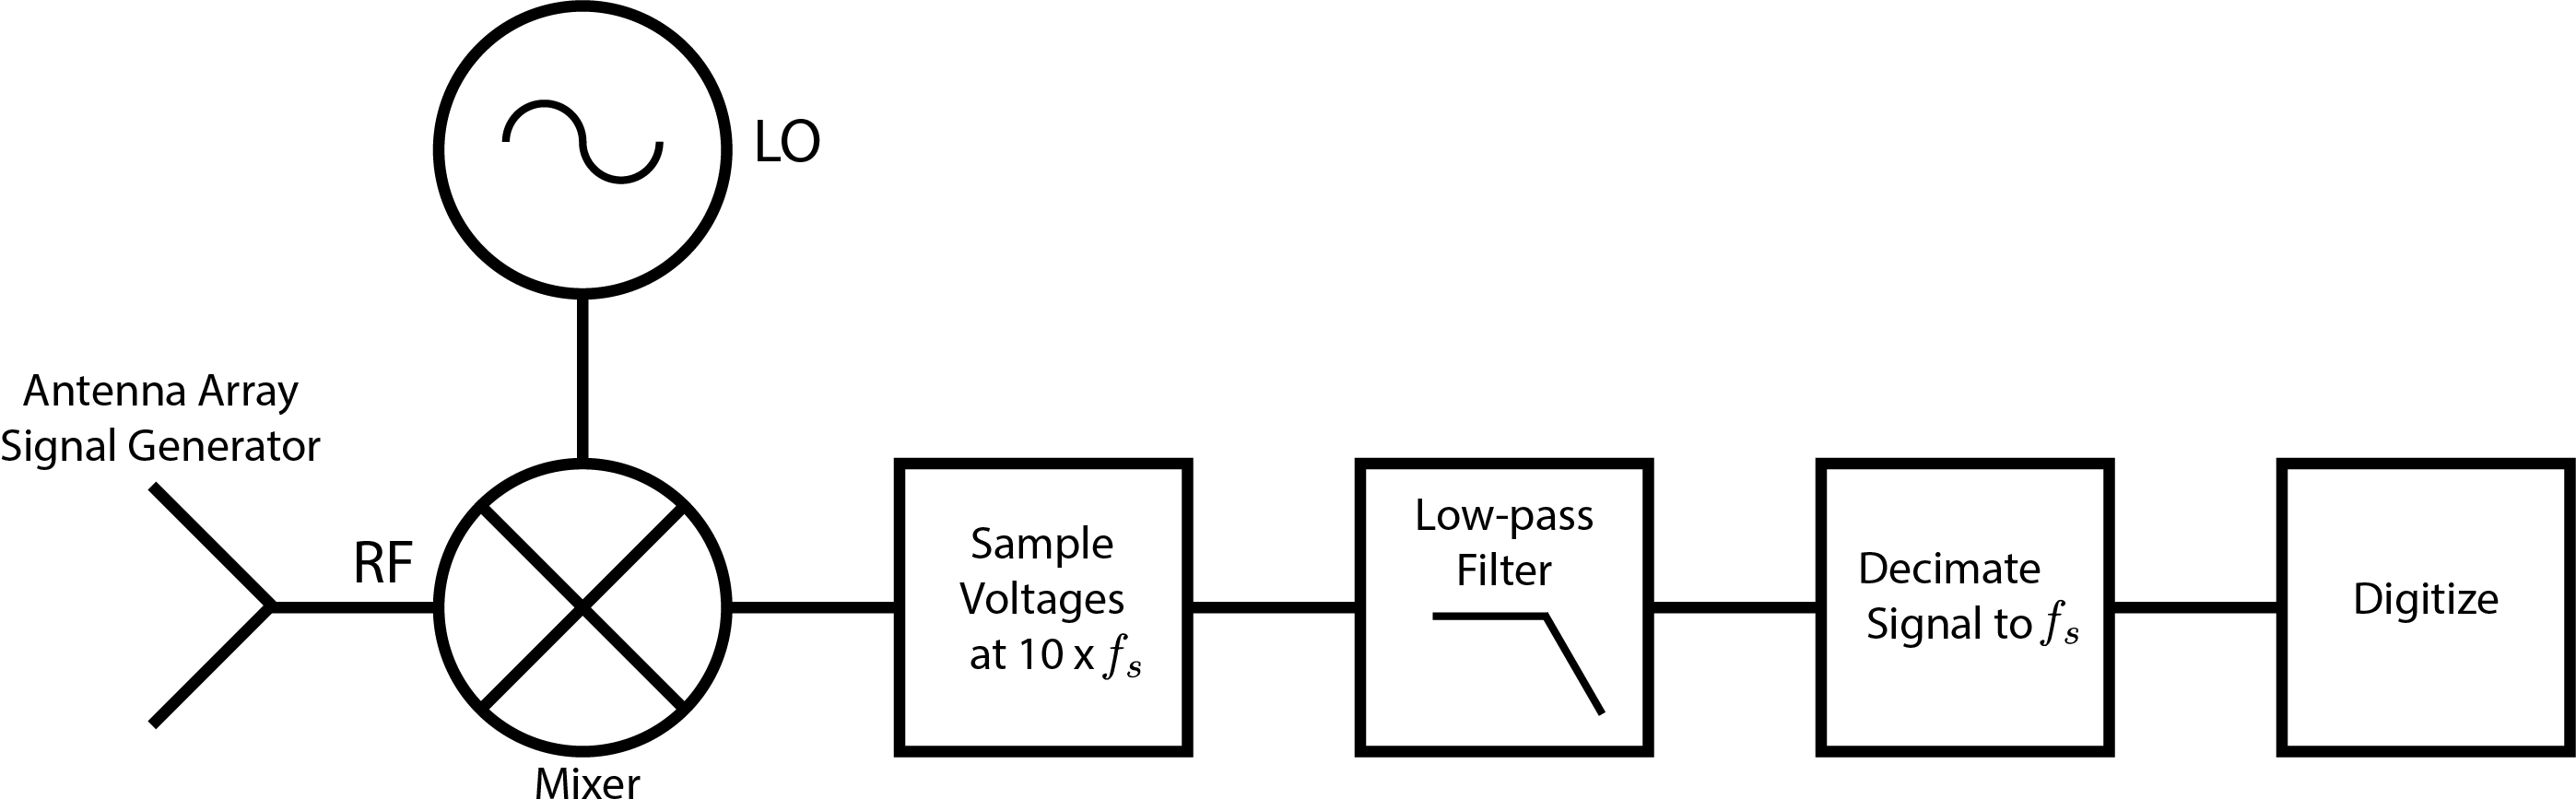
\includegraphics[width=0.85\textwidth]{figs/Chapter-4/230511_locust_receiver_chain.png}
    \caption{The receiver chain used by Locust when simulating CRES events in the FSCD.}
\label{fig:chap4-locust-receiver-chain}
\end{figure}

Frequency down-conversion is used in the FSCD to reduce the digitization bandwidth required to read-out CRES data. According to the Nyquist sampling theorem \cite{nyquist_sampling}, the minimal sampling rate that guarantees no information loss for a signal with a bandwidth $\Delta f$ is given by
\begin{equation}
    f_{\textrm{Nyq}}=2\Delta f.
\end{equation}
The total bandwidth of CRES signal frequencies from tritium beta-decay ranges from 0 to 26~GHz in a $0.95$~T magnetic field, therefore, direct digitization of CRES signals from the FSCD would require sampling frequencies greater than $50$~GHz, which is infeasible for a real experiment. However, for the purposes of neutrino mass measurement we are only interested in measuring the shape of the spectrum in the last 100~eV, which corresponds to a frequency bandwidth of 5~MHz. Down-conversion is a technique for reducing the base frequencies of signals in a bandwidth given by $[f_\textrm{LO},f_\textrm{LO}+\Delta f]$ to the bandwidth $[0, \Delta f]$, by performing the following multiplication
\begin{equation}
    x(t)\rightarrow x(t)e^{-2\pi f_\textrm{LO}}.
\end{equation}
In down-conversion the signal ($x(t)$) is multiplied by a sinusoidal signal with frequency $f_\textrm{LO}$ to reduce the absolute frequencies of the signals in the bandwidth. In the FSCD this allows us to detect events in the last 100~eV of the tritium spectrum while sampling the data far below 50~GHz. The standard bandwidth used in the FSCD is 200~MHz, which allows for higher frequency resolution than the minimum sampling frequency for 100~eV of energy bandwidth.

Trying to directly simulate down-conversion with a frequency multiplication in Locust would require the sampling of the electric fields at each antenna in the FSCD array with a period of $\approx20$~ps, which is extremely slow computationally. To avoid this Locust performs the down-conversion by intentionally under-sampling the electric fields with a frequency of 2~GHz. Sampling below the Nyquist limit causes the higher frequency components of the CRES signal to alias, however, Locust can remove these aliased frequency peaks using a combination of low-pass filtering and decimation to recreate frequency down-conversion. After filtering and decimation, Locust simulates digitization by an 8-bit digitizer at a sampling frequency of 200~MHz to recreate the conditions of the FSCD. The voltage offset and the digitizer range must be configured by the user based on the characteristics of the simulation. 

\subsubsection*{Data}

The output of Locust simulations for the FSCD primarily consists of two data files. The first is the electron trajectory information calculated by Kassiopiea, which is output in the form of a \texttt{.root} file \cite{root}. This file contains important kinematic information about the electron such as it's position and pitch angle as a function of time. The other file is produced by Locust and it contains the digitized signals acquired from each antenna in the FSCD array. The Locust output files conform to the Monarch specification developed by Project 8, which is based on the commonly used HDF5 file format, and matches the format of the files produced by the Project 8 data acquisition software. This makes it possible to use the same data analysis code to analyze both simulated and real data.

\subsection{CRESana}
\label{sec:chap4-cresana}

Locust is the primary simulation tool used by Project 8 in the development and simulation of the FSCD. However, simulations of CRES events in larger antenna arrays ($\geq100$ antennas) using Locust can take several hours to complete, which is prohibitively long when one is performing a sensitivity analysis for a large scale antenna experiment. One of the reasons for Locust's slow operation is that the electric fields from the electron must be solved numerically for each time-step for each of the antennas in the array. These numerical solutions allow Locust to accurately simulate the electric fields from arbitrarily complicated electron trajectories at the cost of more computations and slower simulations. Therefore, an additional simulation tool that sacrifices some accuracy for computational efficiency would be extremely useful simulations and sensitivity analyses of larger antenna array experiments.

To fill this need, Project has developed a new simulations package called CRESana\footnote{\url{https://github.com/MCFlowMace/CRESana}}, specifically designed to perform analytical simulations of antenna array based CRES experiments. CRESana is not as flexible as Locust, but it provides a significant increase in simulation speed. It does this by using well-justified analytical approximations of the electrons motion in the magnetic field and the resulting electric fields from the electron's acceleration. The electric fields and signals generated by CRESana are consistent with theoretical calculations of the electron's radiation, and are test for accuracy using well-known test-case simulations and consistency checks. 

\section{Signal Detection and Reconstruction Techniques for Antenna Array CRES}
\label{sec:chap4-pter}

\subsubsection*{Antenna Array CRES Signal Reconstruction}

A robust set of FSCD simulation tools are vital to the development of the analysis algorithms necessary for antenna array CRES to succeed. In order to perform CRES measurements using an antenna array, one must develop an algorithm that uses the multi-channel time-series obtained by digitizing the array to estimate the starting kinetic energies of electrons produced in the magnetic trap. This procedure consists of a multi-stage process of detecting a CRES signal then estimating the parameters of the electron that produced and is often referred to as simply CRES signal reconstruction.

Compared with the signal reconstruction approaches of the Phase I and II CRES experiments, antenna array CRES requires a significantly different approach to signal reconstruction. In Phase I and II, CRES was performed using a waveguide gas cell that could be directly connected to a waveguide transmission line. The transmission line efficiently transmits the cyclotron radiation along it's length to an antenna at either end of the waveguide. However, with an antenna array the electron is essentially radiating into free-space, therefore, the cyclotron radiation power collected by the array is directly proportional to the solid angle surrounding the electron that is covered with antennas. Because it is not practical to fully surround the magnetic trap with antennas, some of the cyclotron radiation power that would have been collected by the waveguide escapes into free-space. Furthermore, the power that is collected by the antenna array is split between every channel in the antenna array, which significantly lowers the signal-to-noise ratio (SNR) of CRES signals in a single antenna channel compared to a waveguide apparatus. Therefore, a suite of completely new signal reconstruction techniques are needed in order to perform CRES in the FSCD.

Changes to the approach to CRES signal reconstruction are also motivated by the more ambitious scientific goals of the FSCD experiment. A measurement of the tritium beta-decay spectrum that is sensitive to neutrino masses as small as 40~meV requires that we measure the kinetic energies of individual electrons with a total energy broadening of 115~meV \cite{p8bayesian}. This resolution includes all sources of uncertainty in the electron's kinetic energy such as magnetic field inhomogeneities. This level of energy resolution is compatible only with an event-by-event signal reconstruction approach where the kinetic energies, pitch angles, and other parameters of the CRES events are estimated before constructing the beta-decay spectrum. 

The event-by-event approach is distinct from the analysis done for the Phase I and Phase II experiments where only the starting cyclotron frequency of the event was estimated by analyzing the tracks formed by the carrier frequency in the time-frequency spectrogram. These frequencies were then combined into a frequency spectrogram, which was converted to the beta-decay energy spectrum using an ensemble approach that averaged over all other event parameters. The ensemble approach to signal reconstruction results in poor energy resolution because other kinematic parameters such as pitch angle change the cyclotron carrier frequency due to changes in the average magnetic field experience by the electron, and it is therefore incompatible with the future goals of the Project 8 collaboration.

\subsubsection*{Components of Reconstruction: Signal Detection and Parameter Estimation}

CRES signal reconstruction can be viewed as a two-step procedure consisting of signal detection followed by parameter estimation. In the former, one is concerned with identifying CRES signals in the data regardless of the signal parameters, whereas, in the latter one operates under the assumption that a signal is present and then estimates it's parameters. 

More formally, signal detection is essentially a binary hypothesis test between the signal and noise data classes and parameter estimation describes a procedure of fitting a model to the observed data. While both of these processes are required for a complete reconstruction (see Figure \ref{fig:chap4-pter-pipeline}), the focus of my work and this chapter is on the signal detection aspect of antenna array CRES signal reconstruction.

\begin{figure}[htbp]
    \centering
    
\includegraphics[width=0.8\textwidth]{figs/Chapter-4/230108_deepfilter_paper_event_reconstruction_pipeline.png}
    \caption{A high-level diagram depicting the process of CRES event reconstruction. The first step consists of identifying the presence of a signal in the data. This step is necessary to avoid the danger of performing a reconstruction of a false event, which would constitute a background contribution to the tritium spectrum measured by CRES.}
    \label{fig:chap4-pter-pipeline}
\end{figure}

\subsubsection*{Detection Theory}

The problem of signal detection can be posed as a statistical hypothesis test \cite{detection_theory}. For CRES signals, which are essentially vectors with added white Gaussian noise (WGN), one needs to choose between two hypotheses
\begin{align}
    \mathcal{H}_0:&\quad\bm{y}=\bm{\nu}\\
    \mathcal{H}_1:&\quad\bm{y}=\bm{x}+\bm{\nu},
\end{align}
where $\bm{y}$ is the CRES data vector, $\bm{\nu}$ is a sample of WGN, and $\bm{x}$ represents the CRES signal. The hypothesis that the data contains only noise is labeled $\mathcal{H}_0$ and the hypothesis that the data contains a signal is labeled $\mathcal{H}_1$.

For illustrative purposes one can examine the case where one the first sample of data is used to distinguish between $\mathcal{H}_0$ and $\mathcal{H}_1$. The value of the first data sample is distributed according to two gaussian distributions corresponding to $\mathcal{H}_0$ and $\mathcal{H}_1$ (see Figure \ref{fig:chap4-detection-threshold}). By setting a decision threshold on the value of this sample, one can choose the correct hypothesis with a probability given by the areas underneath the probability distributution curves. A true positive corresponds to correctly identifying that the data contains signal, whereas, a true negative means that one has correctly identified the data as noise. The rate at which the detector performs a true positive classification is given by the green region underneath $p(\bm{y}[0];\mathcal{H}_0)$, and the rate at which the detector performs a true negative classification is given by the orange region underneath $p(\bm{y}[0];\mathcal{H}_1)$.
\begin{figure}[htbp]
    \centering
    \begin{subfigure}{0.48\textwidth}
        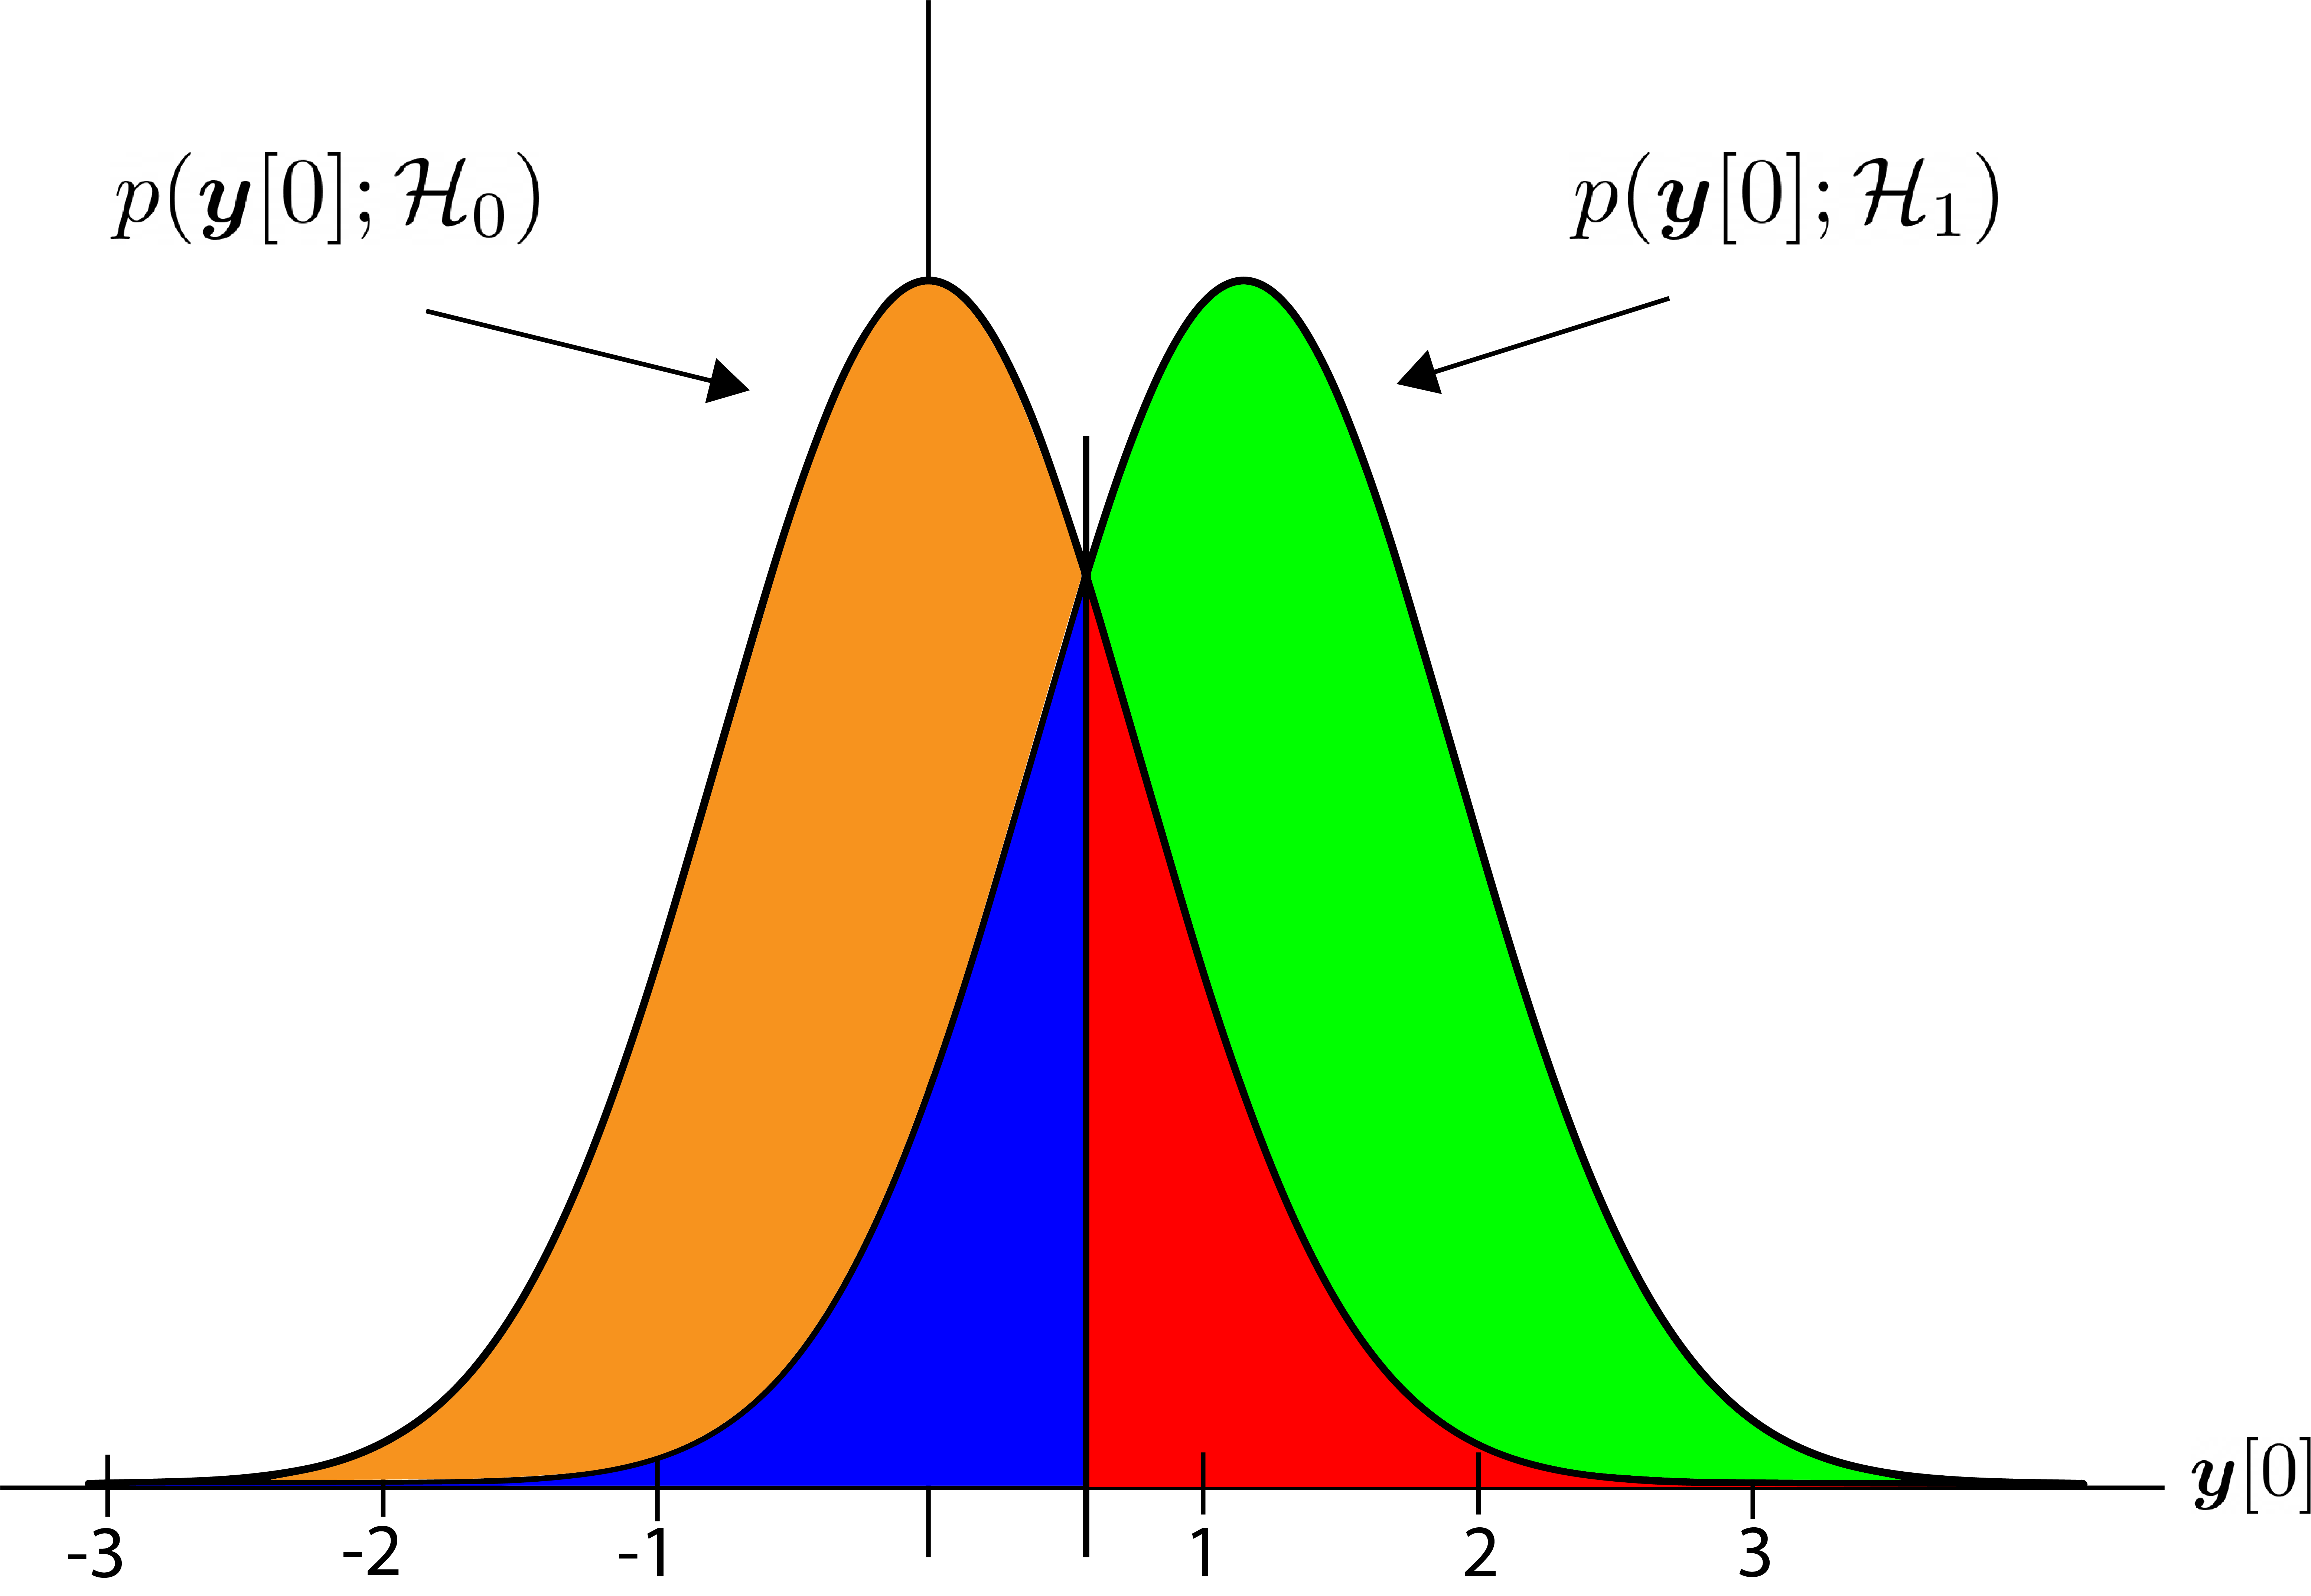
\includegraphics[width=\textwidth]{figs/Chapter-4/230523_detection_theory.png}
        \caption{}
    \end{subfigure}
    \hfill
    \begin{subfigure}{0.48\textwidth}
        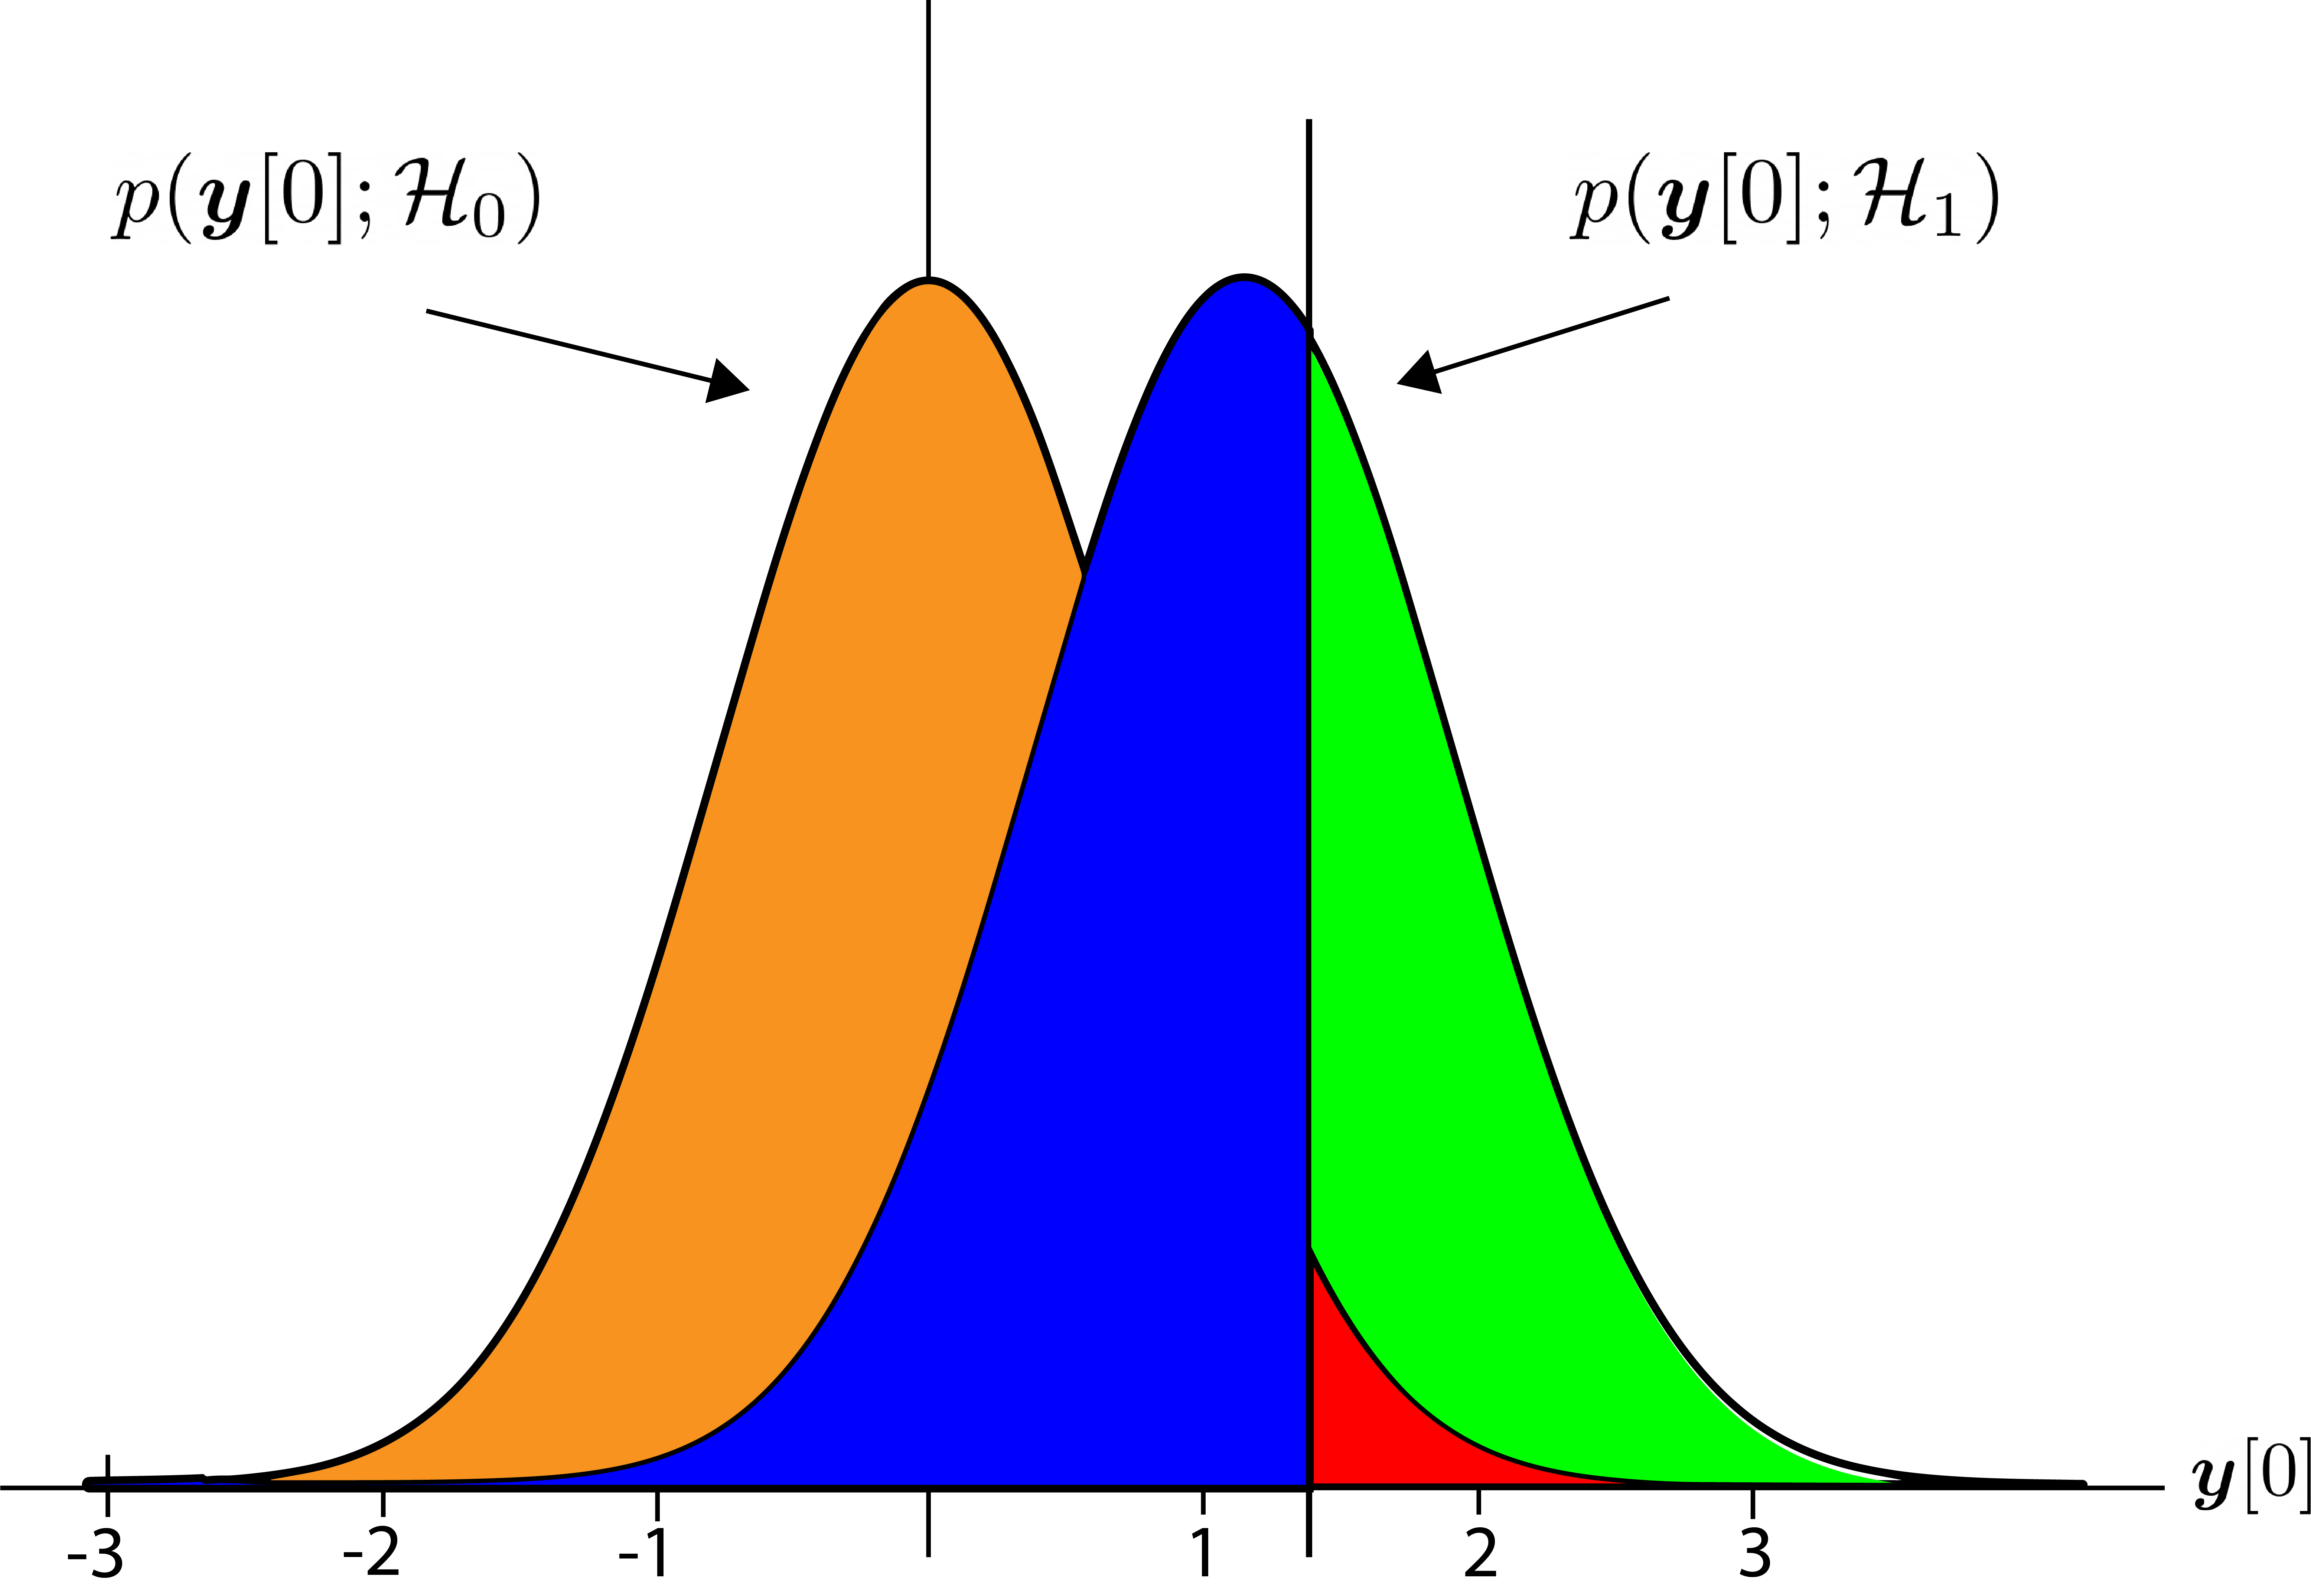
\includegraphics[width=\textwidth]{figs/Chapter-4/230523_detection_theory2.png}
        \caption{}
    \end{subfigure}
    \caption{An illustration of two PDFs associated a binary hypothesis test. The decision threshold is represented by the vertical line that partitions both distributions. The orange and red areas correspond to the true negative and false positive probabilities and the blue and green areas correspond to the false negative and true positive probabilities respectively. To decided between the two hypotheses we perform the likelihood ratio test specified by the Neyman-Pearson theorem. This approach achieves the highest true positive probability for a given false positive probability.}
    \label{fig:chap4-detection-threshold}
\end{figure}
Two types of misclassifications are possible. Either we declare noise data as signal, which is call a false positive, or we declare signal data as noise, which is a false negative. Note that it is only possible to trade off these two types of errors by tuning the detection threshold. One cannot simultaneously reduce the rate of false positives without also increasing the rate of false negatives.

The approach taken with CRES signals is to fix the rate of false positives by setting a minimum value for a detection threshold. The rate of false positives that is acceptable at the detection stage depends upon the rate of background events compatible with the sensitivity goals of the experiment. The ultimate goal of a neutrino mass measurement with 40~meV sensitivity in general has strict requirements on the number of background events, which requires a relatively high detection threshold to achieve. Consequently, the ideal signal detection algorithm is the one that achieves the maximum rate of true positives for a fixed rate of false positives, so that the detection efficiency of the experiment is maximized and potential sources of background are kept to a minimum.

According to the Neyman-Pearson theorem \cite{neyman_pearson_lemma}, the statistical hypothesis test that maximizes the probability of detection for a fixed rate of false positives is the likelihood ratio test, which is formed by computing the ratio of the signal likelihood to the noise likelihood,
\begin{equation}
    L(x)=\frac{P(\bm{y};\mathcal{H}_1)}{P(\bm{y};\mathcal{H}_0)}>\gamma.
\end{equation}
Here, the likelihood of the hypotheses $\mathcal{H}_0$ and $\mathcal{H}_1$ are described by the probability distributions $P(\bm{y};\mathcal{H}_0)$ and $P(\bm{y};\mathcal{H}_1)$ respectively, and $\gamma$ is the threshold for deciding $\mathcal{H}_1$. The decision threshold is determined by integrating $P(\bm{y};\mathcal{H}_0)$ such that 
\begin{equation}
    P_{\textrm{FP}}=\int_\gamma^\infty{P(\tilde{\bm{y}};\mathcal{H}_0)d\tilde{\bm{y}}}=\alpha,
\end{equation}
where $\alpha$ is the desired false positive detection rate given by the red colored areas shown in Figure \ref{fig:chap4-detection-threshold}. The true positive detection rate is given by the similar integral 
\begin{equation}
    P_{\textrm{TP}}=\int_\gamma^\infty{P(\tilde{\bm{y}};\mathcal{H}_1)d\tilde{\bm{y}}},
\end{equation}
which corresponds to the green areas in Figure \ref{fig:chap4-detection-threshold}.

Changing the decision threshold allows one to trade-off between $P_{\textrm{TP}}$ and $P_{textrm{FP}}$ as appropriate for the given situation. It is common to summarize the relationship between $P_{\textrm{TP}}$ and $P_{\textrm{FP}}$ using the receiver operating characteristic (ROC) curve, which is obtained by evaluating the true positive and false positive probabilities as a function of the decision threshold value (see Figure \ref{fig:chap4-example-roc-curve}).
\begin{figure}[htbp]
    \centering
    \includegraphics*[width=0.7\textwidth]{figs/Chapter-4/230603_roc_curve_example.png}
    \caption{\label{fig:chap4-example-roc-curve} An example ROC curve formed by computing the $P_\mathrm{FP}$ and the $P_\mathrm{TP}$ for a given likelihood ratio test. As the decision threshold is increased $P_\mathrm{FP}$ decreases at the expense of a lower $P_\mathrm{TP}$. The black dashed line indicates the lower bound ROC curve obtained by randomly deciding between $\mathcal{H}_0$ and $\mathcal{H}_1$. }
\end{figure}
The ROC curve provides a convenient way to compare the performance of different signal detection algorithms. In general, a classifier with a higher the $P_\mathrm{TP}$ as a function of $P_\mathrm{FP}$ is desirable, which corresponds to a larger area underneath the respective ROC curve. A perfect classifier has an area underneath the curve of 1.0, however, such a classifier is almost never achievable in practice. 

\subsection{Digital Beamforming}
\label{sec:chap4-dig-bf}

\subsubsection*{Introduction to Beamforming}

Beamforming refers to a suite of antenna array signal processing techniques that are designed to enhance the radiation or gain of the array in certain directions and suppress it in other direction \cite{balanis2015antenna}. Beamforming is of interest to Project 8 as a first level of signal reconstruction for the FSCD and other antenna array CRES experiments, which operates at the signal detection stage of reconstruction.% This is because beamforming is designed to combine the outputs of the different antennas in the array into a single signal, that could be analyzed in a similar way as previous CRES experiments to start and provide the basis for the development of new follow-up analysis algorithms.

Beamforming is accomplished by performing a phased summation of the signals received by the antenna array. The beamforming phases are chosen such that the signals emitted by the array will constructively interfere at the point of interest (see Figure \ref{fig:chap4-basic-bf}). As a consequence of the principle of reciprocity \cite{reciprocity_theorem}, when the array is operating in receive mode, the signals emitted from a source at the same point will constructively interfere when summed.  
\begin{figure}[htbp]
    \centering
    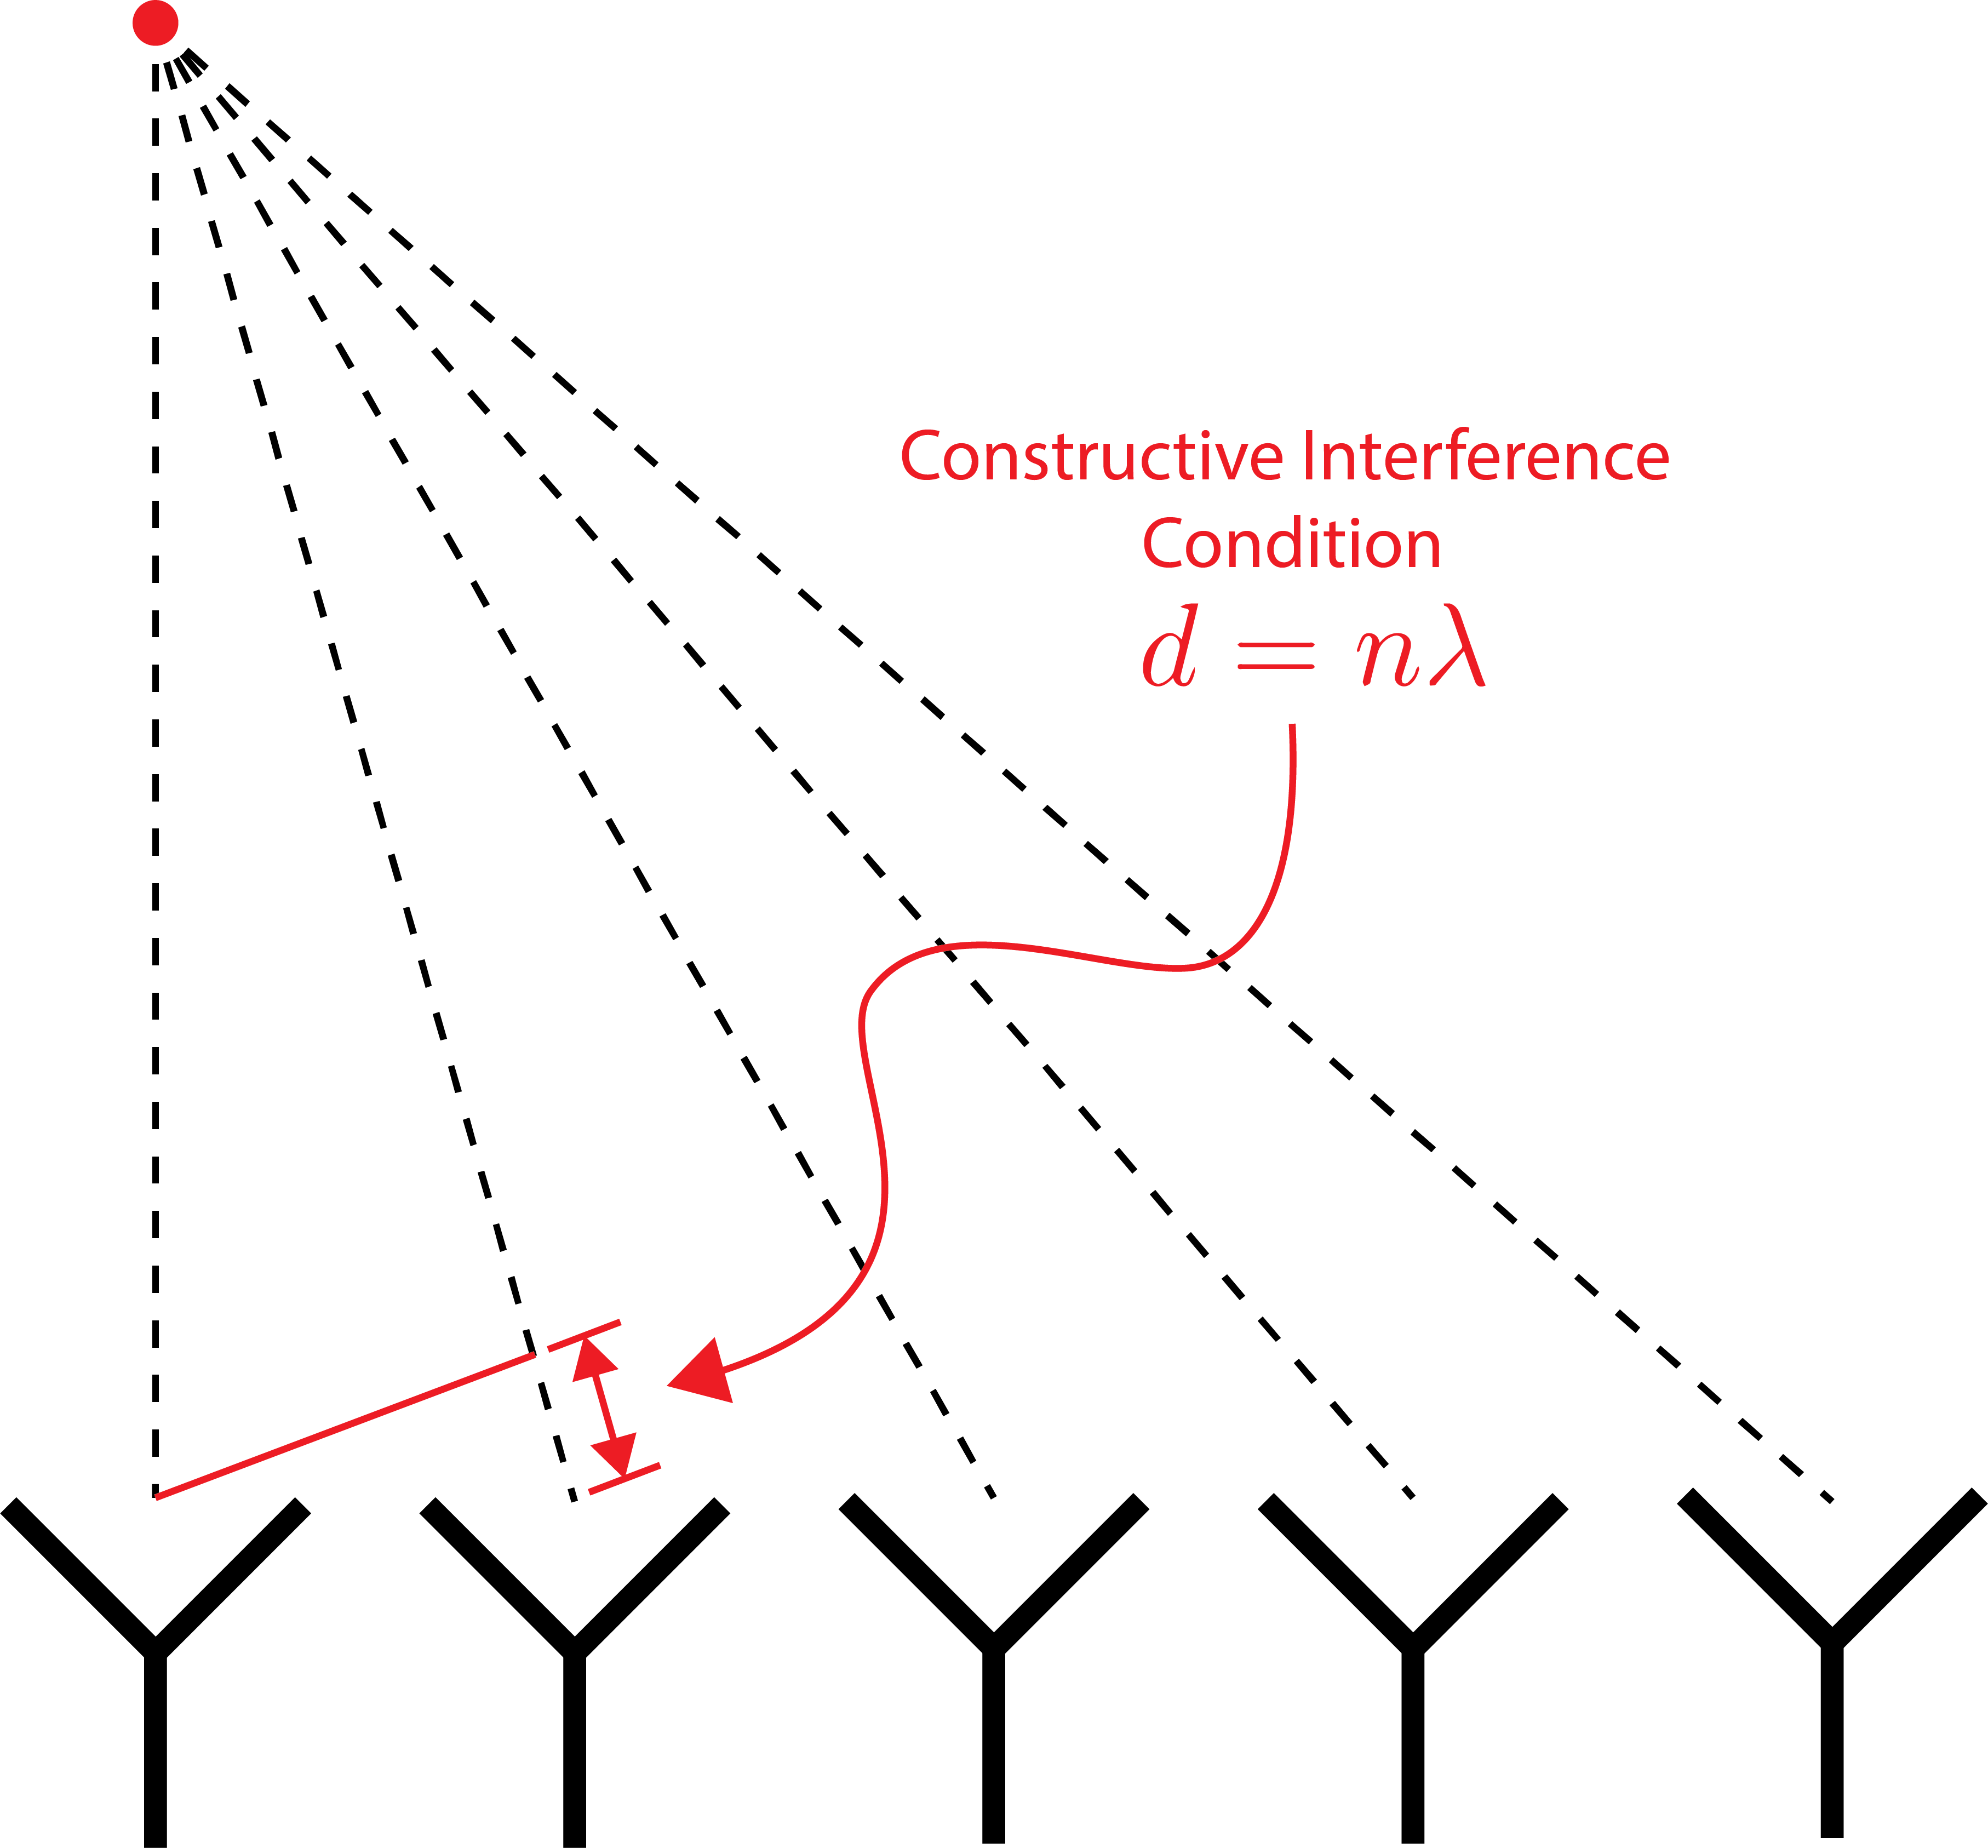
\includegraphics[width=0.6\textwidth]{figs/Chapter-4/230517_basic_bf.png}
    \caption{An illustration of the constructive interference condition which is the operating principle of digital beamforming using a uniform linear array as an example.}
    \label{fig:chap4-basic-bf}
\end{figure}
The origin of the phase delays in beamforming is the path-length difference to the beamforming point between different antennas in the array. The relationship between the phase delay and the path-length difference is given by the familiar equation
\begin{equation}
    \phi=\frac{2\pi d}{\lambda},
    \label{eq:chap4-bf-phases}
\end{equation}
where $\phi$ is the phase delay, $d$ is the path-length difference, and $\lambda$ is the wavelength of the radiation. In practice, one chooses the values of $d$ by specifying the beamforming positions of interest and then calculates the beamforming phases using Equation \ref{eq:chap4-bf-phases}, which is guaranteed to follow the constructive interference condition shown in Figure \ref{fig:chap4-basic-bf}. 

Beamforming can be neatly expressed mathematically using the vector equation
\begin{equation}
    y[n] = \bm{\Phi}^T[n]\bm{x}[n],
\end{equation}
where $\bm{x}[n]$ is the array snapshot vector, $\bm{\Phi}[n]$ is a vector of beamforming shifts, and $y[n]$ is the resulting summed signal. The beamforming shifts consist of a set of complex numbers that contain the beamforming phase shift and an amplitude weighting factor,
\begin{equation}
    \bm{\Phi}[n] = \left[A_0[n]e^{-2\pi i\phi_0[n]}, A_1[n]e^{-2\pi i \phi_1[n]}, ..., A_{N-1}[n]e^{-2\pi i \phi_{N-1}[n]}\right],
\end{equation}
where the set of magnitudes $A_i[n]$ are amplitude weighting factors and $\phi_i[n]$ are the phase shifts from the path-length differences. The index $i$ is used to denote the antenna channel number. The amplitude weighting factor is the relative magnitude of the signal received by a particular antenna to the other antennas in the array, such that the antennas that receive signals with higher amplitude, due to being closer to the source, have more weight in the beamforming summation. The input and outputs signals beamforming are naturally expected to be functions of time as indicated by the index $[n]$, however, it is also possible to use time dependent beamforming phases that shift the beamforming position of the array over time.

Digital beamforming is the type of beamforming algorithm of interest to Project 8 for CRES. Specifically, digital beamforming means that the beamforming phases are applied to the array signals in software rather than employing fixed beamforming phase shifts in the receiver chain hardware. The advantage of digital beamforming is that for a given series of array snapshots one can specify a large number of beamforming positions and effectively search for electrons by performing the beamforming summation associated with each point and applying a signal detection algorithm to identify the presence of a CRES signal.

One of the most attractive features of digital beamforming is the spatial filtering effect, which is a direct consequence of the constructive interference condition used to define the beamforming phases. Spatial filtering allows for signals from multiple electrons at different positions in the trap to be effectively separated, because the constructive interference condition will force the signals from electrons at positions different from the beamforming position to cancel. This helps to reduce signal pile-up that could become an issue for large scale CRES experiments using a dense tritium source.

The digital beamforming positions can be specified with arbitrary densities limited only by the available computational resources. This provides a very straight-forward way to estimate the position of the electron in the trap by using a dense grid of beamforming positions and maximizing the output power of the beamforming summation over this grid. This natural approach to position reconstruction is attractive due the requirements of an event-by-event signal reconstruction, which needs an accurate estimation of the exact magnetic field experienced by the electron in order to correctly estimate it's kinetic energy. Combined with an accurate map of the magnetic field inhomogeneities of the trap obtained from calibrations, beamforming allows one to apply this magnetic field correction with a spatial resolution that is a fraction of the cyclotron wavelength.

\subsubsection*{Laboratory Beamforming Demonstrations}

\begin{figure}[htbp]
    \centering
    \includegraphics*[width=0.7\textwidth]{figs/Chapter-4/230725_beamforming_setup_diagram.png}
    \caption{\label{fig:chap4-beamforming-demo-system}System level diagram of the laboratory setup used for beamforming demonstrations at Penn State. For more information on this system see Chapter 5. Signals near 26~GHz are fed to a dipole antenna using and arbitrary waveform generator (AWG) and vector network analyzer (VNA), which drive a mixer. The dipole radiation is collected by an array of antennas connected to the digitizer data acquisition (DAQ) system.}
\end{figure}

As part of the development of antenna array CRES for the FSCD, an antenna measurement setup was constructed at Penn State to serve as a testbed for antenna prototypes and to perform laboratory validations of array simulations. This system is discussed in more detail in Chapter 5. Early versions of the antenna measurement system (see Figure \ref{fig:chap4-beamforming-demo-system} and Figure \ref{fig:chap4-beamforming-demo-photos}) were used to perform beamforming reconstruction studies of a simple probe antenna to better understand the principles of beamforming and confirm the estimated beamforming performance of Locust.

\begin{figure}
    \centering
    \includegraphics*[width=0.7\textwidth]{figs/Chapter-4/230725_beamforming_demo_image.png}
    \caption{\label{fig:chap4-beamforming-demo-photos}Photographs of the beamforming demonstration setup. In (a) I show a top-down view of the dipole antenna and the array of eight horn antennas. Manual repositioning of the horn antennas allows one to synthesize a full-circular antenna array. The dipole antenna is mounted on a camera tripod mount that allows for manual position tuning. (b) is a close up image of the dipole, which is manufactured from two segments of semi-rigid coaxial cable. (c) is another image of the dipole and array.}
\end{figure}

Signals from an arbitrary waveform generator were up-converted to 26~GHz using a mixer and a high-frequency source from a vector network analyzer and fed to the dipole antenna through a balun. The radiation from the dipole antenna was received by an array of horn antennas. The signals from the horn antennas were then down-converted to baseband using a collection of mixers and an 8-way power divider. The signals were then digitized and saved to a host computer for analysis.

\begin{figure}
    \centering
    \includegraphics*[width=0.85\textwidth]{figs/Chapter-4/230725_beamforming_example.png}
    \caption{\label{fig:chap4-beamforming-demo-example}An example of digital beamforming reconstruction of a dipole antenna using a synthetic array of horn antennas. The beamforming image on the right is constructed by computing the time-averaged power of the summed signals for a two-dimensional grid of beamforming positions. In the image one can see a clear maximum that corresponds to the position of the dipole antenna. On the left I show the frequency spectrum of the time-series at the maximum power pixel. White gaussian noise is added to the signal to mimic a more realistic signal-to-noise-ratio. The signal emitted by the dipole is clearly visible as the high power peak in the frequency spectrum.}
\end{figure}

The data collected using the dipole and horn antenna array is reconstructed using the beamforming reconstruction approach specified in Section \ref{sec:chap4-dig-bf}. A two-dimensional grid of xy-positions is defined and the beamforming phase shifts for each of these positions is calculated. The phased summation can be visualized by plotting the time-averaged power for each of the summations as a pixel in the resulting beamforming image (see Figure \ref{fig:chap4-beamforming-demo-example}). White Gaussian noise (WGN) can be added to the data at this stage to simulate more realistic signal-to-noise ratios (SNR) if desired. The beamforming peak maxima is expected to have a Bessel function shape due to the circular symmetry of the array, and by analyzing the size of the beamforming maxima one can confirm that the beamforming reconstruction measurement has similar position resolution as expected from Locust simulations. Additionally, signal detection rates can be estimated from the data by comparing the magnitude of the beamforming signal peak in the frequency spectra to simulation.


\subsubsection*{FSCD Beamforming Simulations}

Using Locust simulations of the FSCD one can perform beamforming reconstruction studies using the simulated CRES signal data. As we mentioned in the previous section, the beamforming procedure beings by specifying a set of beamforming positions and corresponding beamforming shifts. The beamforming positions form a grid that covers the region of interest in the field of view of the antenna array. There are effectively an infinite number of ways to specify the grid positions, however, uniform square grids are the most commonly used due to their simplicity. In the FSCD experiment the number and pattern of the grid positions would be optimized to cover the most important regions of the trap volume to maximize detection efficiency while minimizing superfluous calculations.

\begin{figure}[htbp]
    \centering
    \begin{subfigure}{0.45\textwidth}
        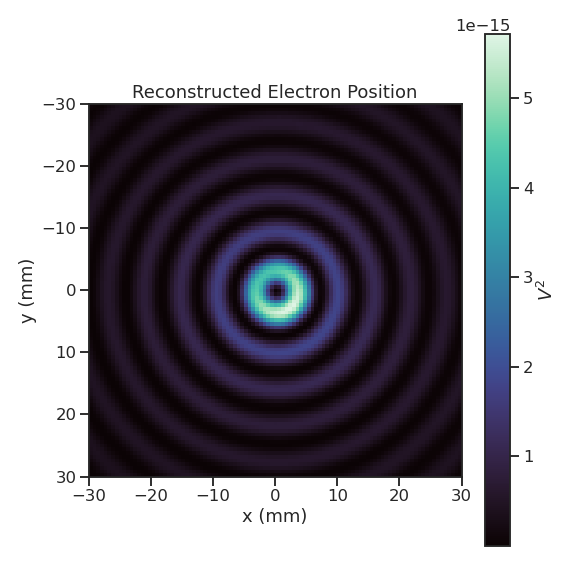
\includegraphics[width=\textwidth]{figs/Chapter-4/230518_locust_bf_onaxis_no_cyclotron.png}
        \caption{\label{fig:chap4-bf-no-cyc-phase-ex}}
    \end{subfigure}
    \hfill
    \begin{subfigure}{0.45\textwidth}
        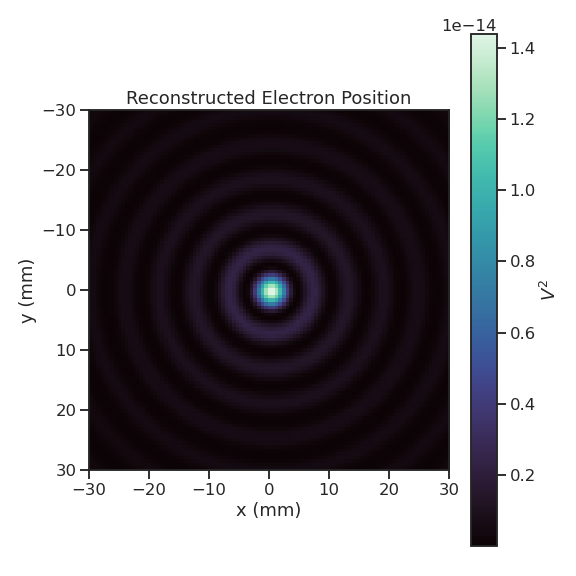
\includegraphics[width=\textwidth]{figs/Chapter-4/230518_locust_bf_onaxis.png}
        \caption{}
    \end{subfigure}
    \caption{Beamforming images visualizing the reconstruction of an electron without (a) and with (b) the cyclotron phase correction. The images were generated using data from Locust simulations. The cyclotron phase refers to a phase offset equal to the relative azimuthal position of an antenna in the array. This phase offset is caused by the circular electron orbit and must be corrected for during reconstruction.}
    \label{fig:chap4-cyclotron-phase-bf-corr}
\end{figure}

The beamforming grids used for signal reconstruction with the FSCD consist of a set of points that cover a region of the two-dimensional plane formed by the perimeter of the antenna array. The axial dimension is left out of the beamforming grid because the electrons are assumed to occupy only an average axial position, which corresponds to the center of the magnetic trap. This is because it is impossible to resolve the axial position of the electron as a function of time due to the rapid axial oscillation frequencies of trapped electrons relative to the FSCD time-slice duration.

After beamforming, a summed time-series is obtained for each beamforming position that can be evaluated for the presence of a signal using a detection algorithm. A beamforming image is a visualization method that is equivalent to arranging the beamforming grid points according to their physical locations to form a three-dimensional matrix where the first two dimensions encode the XY-position of the beamforming point and the third dimension contains the summed time-series. The image is formed by taking the time-averaged power (see Figure \ref{fig:chap4-cyclotron-phase-bf-corr}). Beamforming images are purely for the purposes of visualization and are not particularly useful for signal detection or reconstruction.

If the beamforming phases consist only of the spatial phase component from Equation \ref{eq:chap4-bf-phases}, then the resulting beamforming image contains a relatively high-power ring-shaped region that is centered on the position of the electron (see Figure \ref{fig:chap4-bf-no-cyc-phase-ex}). The origin of this shape is an additional phase offset particular to a cyclotron radiation source. Essentially, the circular motion that produces the cyclotron radiation introduces a relative phase offset to the electric fields that is equal to the azimuthal position of the field measurement point. For example, if we have two antennas, one located at an azimuthal position of $0^\circ$ and another located at an azimuthal position of $90^\circ$, then the CRES signals received by these antennas will be out of phase by $90^\circ$, which is the difference in their azimuthal positions. This phase offset can be corrected by adding an additional term to the beamforming phase equation that is equal to the azimuthal position of the antenna relative to the electron, 
\begin{equation}
    \phi_i[n] = \frac{2\pi d_i[n]}{\lambda} + \Delta\varphi_i[n],
\end{equation}
where $\Delta\varphi_i$ is difference between the azimuthal position of the electron and the $i$-th antenna channel. Using the updated beamforming phases in the summation changes the ring feature into a Bessel function peak whose maximum corresponds to the position of the electron. Including this cyclotron phase correction significantly improves the signal detection and reconstruction capabilities of beamforming by more than doubling the summed signal power and shrinking the beamforming maxima feature size. 

The beamforming image examples in Figure \ref{fig:chap4-cyclotron-phase-bf-corr} were produced using an electron located on the central axis of the magnetic trap, which do not experience $\nabla B$-drift. However, for electrons produced at non-zero radial position the beamforming phases must be made time-dependent in order to track the position of the electron's guiding center over time. Without this correction the $\nabla B$-drift causes the electron to move between beamforming positions, which effectively spreads the cyclotron radiation power over a wider area in the beamforming image (see Figure \ref{fig:chap4-gradb-bf-drift-corr}).
\begin{figure}[htbp]
    \centering
    \begin{subfigure}{0.45\textwidth}
        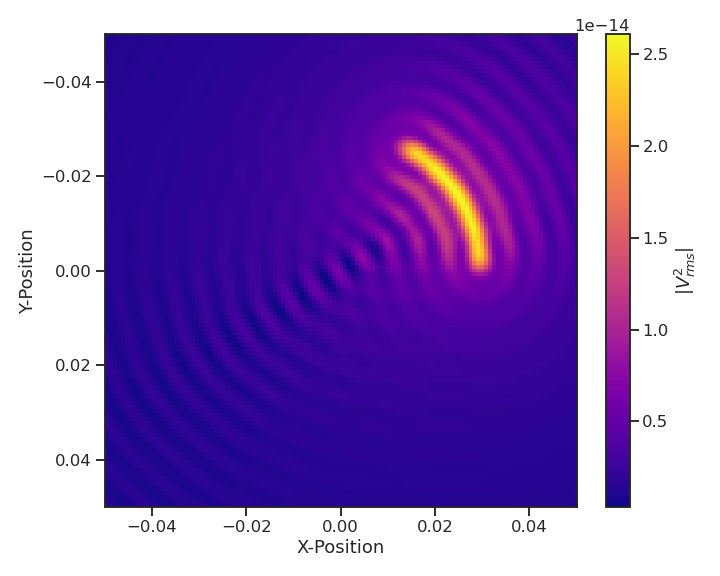
\includegraphics[width=\textwidth]{figs/Chapter-4/220318_88deg_electron_3cm_no_correction.png}
        \caption{}
    \end{subfigure}
    \hfill
    \begin{subfigure}{0.45\textwidth}
        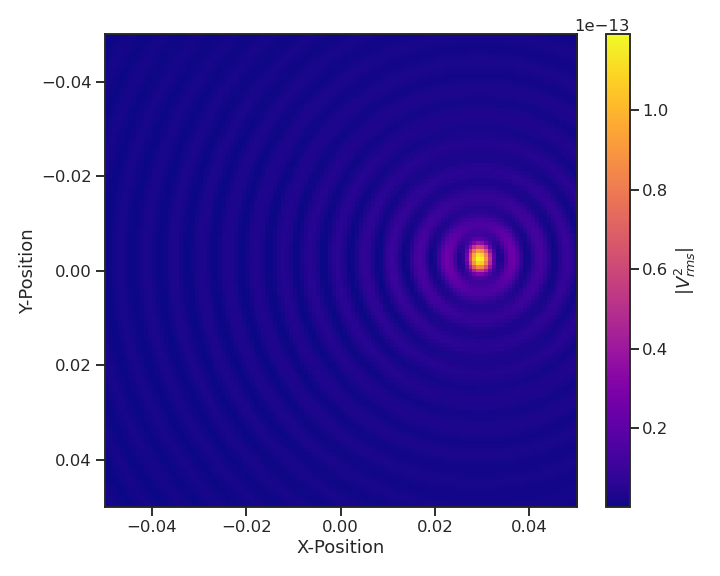
\includegraphics[width=\textwidth]{figs/Chapter-4/220318_88deg_electron_3cm_corrected.png}
        \caption{}
    \end{subfigure}
    \caption{Beamforming images visualizing the reconstruction of an electron located off the central axis of the FSCD trap. In (a) we performing beamforming without the $\nabla B$-drift correction, and in (b) we include the $\nabla B$-drift correction.}
    \label{fig:chap4-gradb-bf-drift-corr}
\end{figure}
This effect significantly reduces the power of the beamforming maxima and increases the size of the beamforming features, simultaneously harming detection efficiency and position reconstruction. 

The $\nabla B$-drift correction simply adds a circular time-dependence to the beamforming positions as a function of time,
\begin{align}
    r[n]&=r_0\\
    \varphi[n]&=\varphi_0 + \omega_{\nabla B}t[n], 
\end{align}
where $\omega_{\nabla B}$ is the drift frequency and $t[n]$ is the time vector. In the ideal case the $\nabla B$-drift frequencies from Figure \ref{fig:chap4-gradb-drift-frequency-map} for the correct pitch angle and radial position would be used, however, it is not possible to know the electron's pitch angle a priori. In principle, one could perform multiple beamforming summations for a given beamforming position using different drift frequencies and choose the one that maximizes the summed power, but this approach leads to a huge computational burden that would be impractical for a real FSCD experiment. A compromise is to use an average value of $\omega_{\nabla B}$ obtained by averaging over the drift frequencies for electrons of different pitch angle at a particular radius. This approach keeps the computational cost of time-dependent beamforming to a minimum while still providing a significant increase in the detection efficiency of digital beamforming.

\subsubsection*{Signal Detection with Beamforming and a Power Threshold}

Up to this point we have neglected any specific discussion of how digital beamforming is used for signal detection and reconstruction. This is because, strictly speaking, digital beamforming consists only of the phased summation of the array signals and cannot be used alone for signal detection. The example beamforming images shown in Figure \ref{fig:chap4-cyclotron-phase-bf-corr} and Figure \ref{fig:chap4-gradb-bf-drift-corr} were produced using simulated data that contained no noise, which significantly degrades the utility of analyzing the beamforming images for signal detection and reconstruction. 

\begin{figure}[htbp]
    \centering
    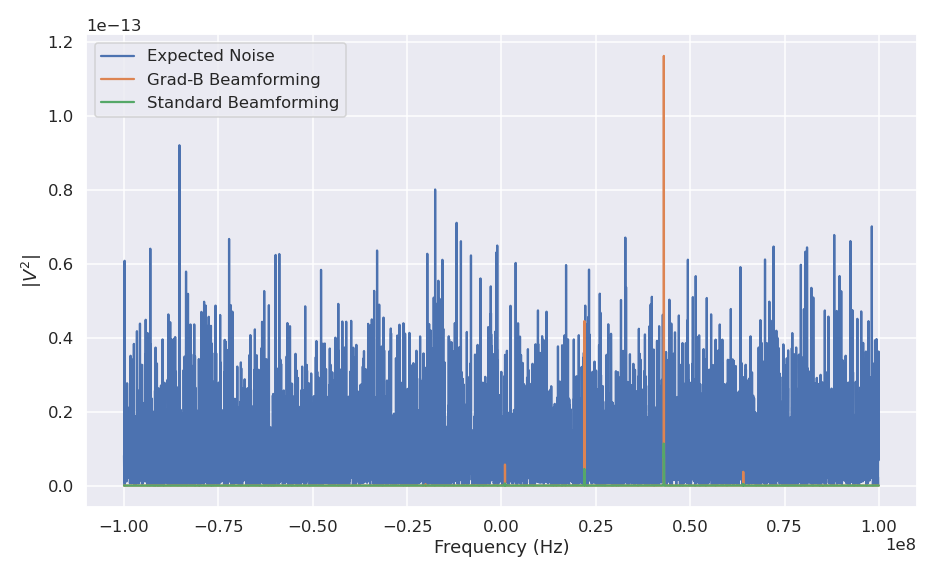
\includegraphics[width=0.67\textwidth]{figs/Chapter-4/220304_example_power_spectrum_gradb_vs_noise_vs_standard_bf.png}
    \caption{A plot of a typical frequency spectrum obtained by applying a Fourier transform to the time-series obtained from beamforming. The frequency spectra are plotted without noise on top of an example of a typical noise spectrum to visualize a realistic signal-to-noise ratio. In the example we see that without beamforming it would not be possible to detect anything since the signal amplitudes would be reduced by a factor of sixty relative to the noise. Additionally, we see that the $\nabla B$-drift correction is needed to detect this electron since it comes from a simulation of an electron with a significant off-axis position. }
    \label{fig:chap4-bf-signal-example}
\end{figure}

Digital beamforming as a detection algorithm is understood to mean digital beamforming plus a detection threshold placed on the amplitude of the frequency spectrum obtained by applying a fast Fourier transform (FFT) to the summed time-series (see Figure \ref{fig:chap4-bf-signal-example}). This approach is most similar to the time-frequency spectrogram analysis employed in previous CRES experiments, however, in principle any signal detection algorithm could be used after the beamforming procedure. In Section \ref{sec:chap4-trigger-paper} I analyze the signal detection performance of the power threshold approach in detail.

From the example frequency spectra in Figure \ref{fig:chap4-bf-signal-example} it is clear that without a reconstruction technique that coherently combines the signals from the full antenna our ability to detect CRES signals will be drastically reduced. Because the CRES signals are in-phase at the correct beamforming position the summed power increases as a function of $N^2$ compared to a single antenna channel, where $N$ is the number of antennas. It is true that the noise power is also increased by beamforming, but, because the noise is incoherent, it's power only increases linearly. Consequently, the signal-to-noise ratio (SNR) of the CRES signal increases linearly with the number of antennas, which greatly improves detection efficiency compared to using only the information in a single antenna.

\begin{figure}[htbp]
    \centering
    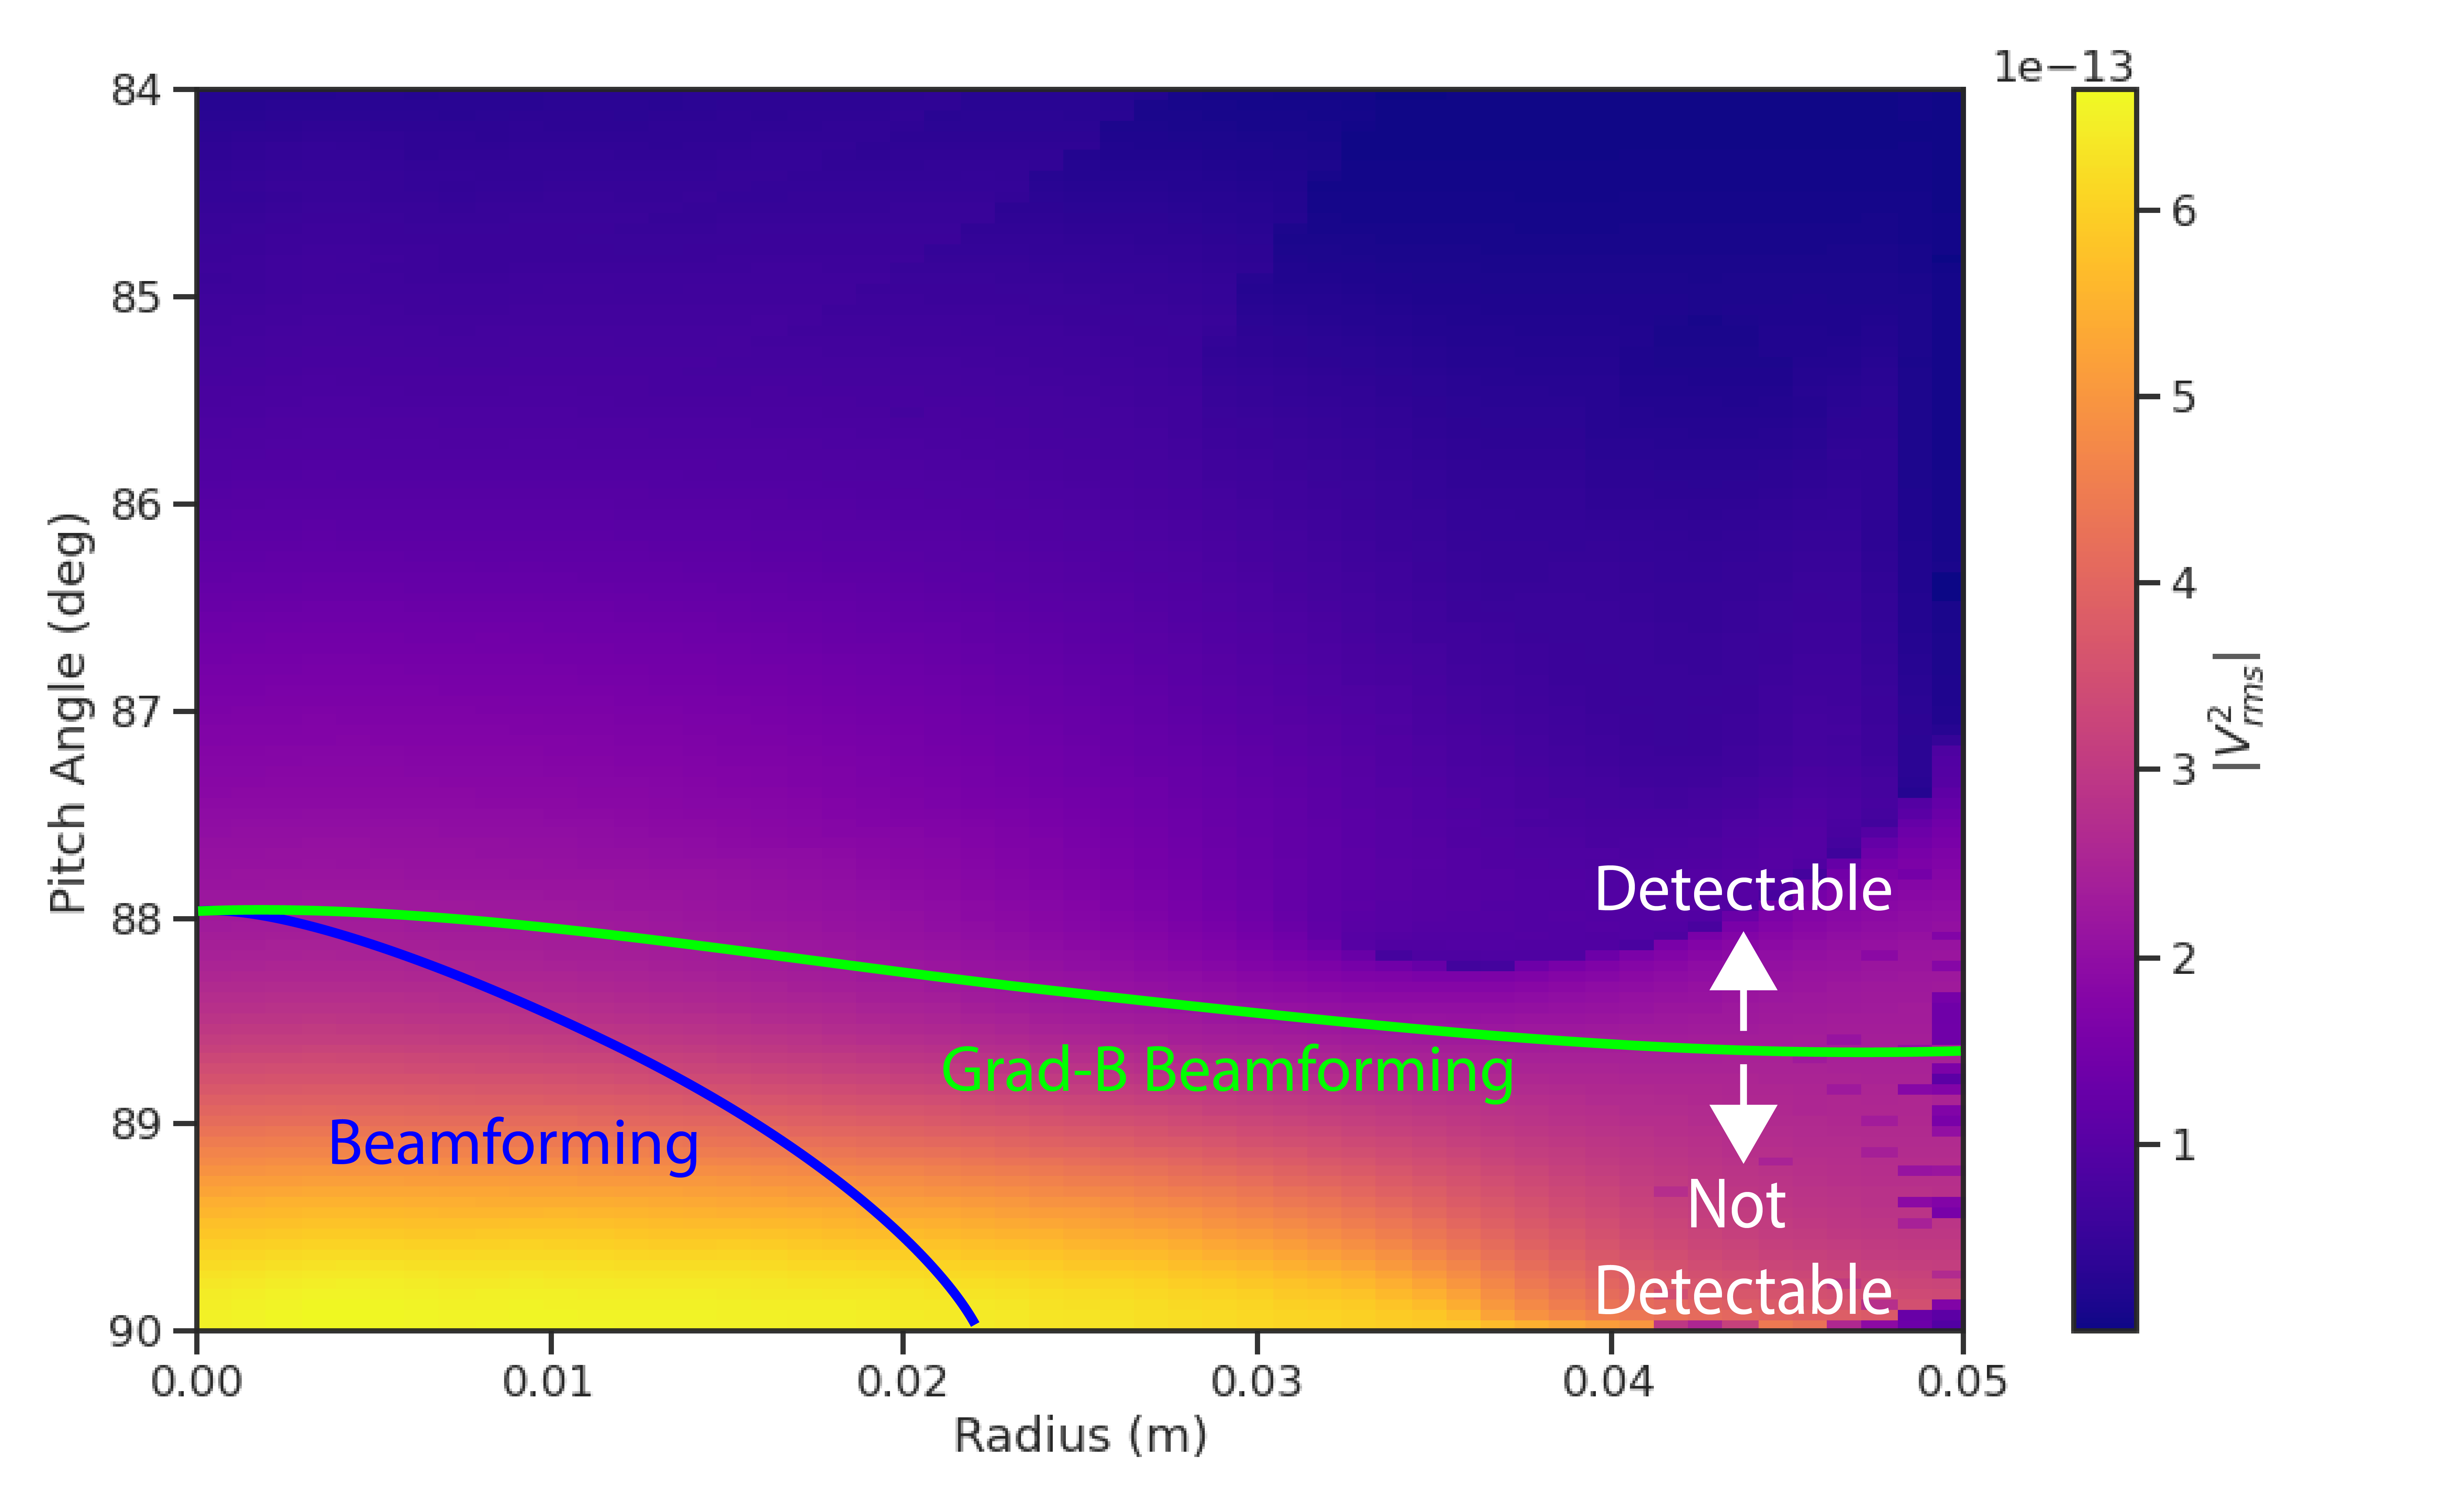
\includegraphics[width=0.67\textwidth]{figs/Chapter-4/230522_beamforming_detectability.png}
    \caption{A plot of the total signal power received by the FSCD array from trapped electrons with different radial positions and pitch angles generated using Locust simulations. The lines on the plot indicate a 10~dB detection threshold above the mean value of the noise in the frequency spectrum. With static beamforming electrons with radial positions larger than about two centimeters are undetectable due to the change in the electron's position over time causing losses from beamforming phase mismatch. This is corrected by including $\nabla B$-drift frequencies in the beamforming phases. Both beamforming techniques fail to detect electrons below $\approx 88.0^\circ$, since these signal are composed of several relatively weak sidebands that are comparable to the noise.}
    \label{fig:chap4-detection-boundaries}
\end{figure}

The power threshold detection algorithm searches for high-power frequency bins that should correspond to a frequency component of the CRES signal. In order to prevent random noise fluctuations from being mistaken as CRES signals the power threshold must be set high enough so that it is unlikely that random noise could be responsible. A consequence of this is that many electrons that can be trapped will go undetected because the modulation caused by axial oscillations leads to the cyclotron carrier power to falling below the decision threshold. The time-dependent beamforming used to correct for the $\nabla B$-drift increases the volume of the magnetic trap where electrons can be detected, but it is ineffective at increasing the range of detectable pitch angles (see Figure \ref{fig:chap4-detection-boundaries}). Fundamentally, this is because the power threshold only uses a fraction of the signal power to detect electrons and ignores the power present in the frequency sidebands. In the subsequent sections I examine two other signal detection algorithms that seek to improve the detection efficiency of the FSCD by utilizing the more of the signal shape to compute the detection test statistics.

\subsection{Matched Filtering}

\subsubsection*{Introduction to Matched Filtering}

The problem of CRES signal detection is the problem of detecting a signal buried in WGN, which has been examined at great depth in the signal processing literature \cite{detection_theory}. For a fully known signal in WGN the optimal detector is the matched filter, which means that it achieves the highest true positive rate for a fixed rate of false positives. The matched filter test statistic is calculated by taking the inner product of the data with the matched filter template
\begin{equation}
    \mathcal{T}=\left|\sum_{n}{h^\dagger[n]y[n]}\right|,
    \label{eq:chap4-mf-test-stat-perfect}
\end{equation}
where $h[n]$ is the matched filter template and $y[n]$ is the data. The matched filter test statistic defines a binary hypothesis test in which the data vector is assumed to be an instance of two possible data classes. By setting a decision threshold on the value of $\mathcal{T}$, one can classify a given data vector as belonging to two distinct hypotheses. Under the first hypothesis the data is composed of pure WGN, and under the second hypothesis the data is composed of the known signal with additive WGN. The matched filter template is obtained by rescaling the known signal in the following way
\begin{equation}
    h[n] = \frac{x[n]}{\sqrt{\tau \sum_{n}{x^\dagger[n]x[n]}}},
    \label{eq:chap4-mf-template-definition}
\end{equation}
where $\tau$ is the variance of the WGN and $x[n]$ is the known signal. Strictly speaking, Equation \ref{eq:chap4-mf-template-definition} is only true for noise with a diagonal covariance matrix, however, in the context of the FSCD we are justified in assuming this to be true. Defining the matched filter templates in this way guarantees that the expectation value of $\mathcal{T}$ is equal to one when the data contains only noise, which is the standard matched filter normalization in the signal processing literature.

Although matched filters are canonically formulated in terms of a perfectly known signal, it is still possible to apply the matched filter technique given imperfect information about the signal provided that the signal is deterministic. From our discussion of CRES simulation tools for the FSCD (see Section \ref{sec:chap4-simulations}) we know that the shape of CRES signals are completely determined by the initial parameters of the electron. The random collisions with background gas molecules which cause the formation of signal tracks are the only stochastic component of the CRES event after the initial beta-decay, therefore, it is possible to develop a matched filter for the detection of CRES signal tracks which are fully determined by the parameters of the electron after the initial beta-decay or subsequent collision events.

\begin{figure}[htbp]
    \centering
    \includegraphics*[width=0.7\textwidth]{figs/Chapter-4/220318_example_convolution.png}
    \caption{Example of a convolution of a CRES signal template with a segment of noisy data. A simulated CRES signal was simulated using Locust and normalized to create a matched filter template. When this template is convolved with noisy data the contains the matching signal the convolution output increases dramatically compared to data with only noise. The decreasing convolution output as the time offset of the convolution increases is caused by zero-padding of the data and template. }
\end{figure}

The matched filter test statistic for CRES signals is a modified version of Equation \ref{eq:chap4-mf-test-stat-perfect}
\begin{equation}
    \mathcal{T} = \max_{\bm{h},m}\left|\bm{h}\ast\bm{y}\right|=\max_{\bm{h},m}\left|\sum_{k}h^\dagger[k]x[m-k]\right|,
    \label{eq:chap4-mf-test-stat-conv}
\end{equation}
where the matched filter inner product has been replaced with a convolution operation and a maximization over the template and convolution delay ($m$). Replacing the inner product with a convolution accounts for the fact that the start time of the CRES signal is now an unknown parameter, in addition, we now perform a maximization of the matched filter convolution over a number of different templates. Because the shape of the signal is unknown we are forced to guess a number of different signal shapes to create a template bank with which we can identify unknown signals by performing an exhaustive search.

The template bank approach to matched filtering, while quite powerful, can quickly become computationally intractable. This is especially true in the case of the FSCD because of the large amount of raw data produced by the array that must be analyzed. Specifically, the time-domain convolution specified by Equation \ref{eq:chap4-mf-test-stat-conv} is particularly computationally intensive and is a major barrier towards the implementation of a matched filter for signal detection in an experiment like the FSCD. This can be avoided by using the convolution theorem to replace the time-domain convolution with an inner product in the frequency domain. 

The convolution theorem states that 
\begin{equation}
    \bm{f}\ast\bm{g} = \mathcal{F}^{-1}\left(\bm{F}\cdot \bm{G}\right)
    \label{eq:chap4-conv-theorem}
\end{equation}
where $\bm{f}$ and $\bm{g}$ are discretely sampled time-series, $\bm{F}$ and $\bm{G}$ are the respective discrete Fourier transforms, and $\mathcal{F}^{-1}$ is the inverse discrete Fourier transform operator. The convolution theorem allows us to perform the matched filter convolution by first computing the Fourier transform of the template and data, then performing a point-wise multiplication of the two frequency series, and finally performing the inverse Fourier transform to obtain the convolution output. Because discrete Fourier transforms can be performed extremely efficiently, the convolution theorem is almost always used in lieu of directly computing the convolution. 

One thing to note here is that the convolution theorem for discrete sequences shown here, is technically valid only for circular convolutions, which is not directly specified in Equation \ref{eq:chap4-mf-test-stat-conv}. However, because typical CRES track lengths are much longer than the Fourier analysis window and also that the frequency chirp rates are small compared to the time-slice duration, it is relatively safe to use circular convolutions to evaluate matched filter scores for CRES signals, which allows us to apply the convolution theorem to compute matched filter scores using the frequency representation of the data and matched filter template.

\subsubsection*{Matched Filter Analysis of the FSCD}

The optimality provided by the matched filter makes it a useful algorithm for analysis of CRES experiment designs for sensitivity analyses, since it indicates the best possible detection efficiency achievable by an experiment configuration. The standard approach to performing these studies involves generating a large number of simulated electron signals that span the kinematic parameter space of electrons in the magnetic trap. In general, electrons have six kinematic parameters along with an additional start time parameter. 

In order to limit the number of simulations required to evaluate the detection efficiency the standard approach is to fix the starting axial position, starting azimuthal position, starting direction of the perpendicular component of the electron's momentum, and event start time to reduce the parameter space to starting radial position, starting kinetic energy, and starting pitch angle. The fixed variables are true nuisance parameters that do not affect the detection efficiency estimates for the FSCD design, because they manifest as phases which are marginalized during the calculation of the matched filter score.

Across radial position, kinetic energy, and pitch angle one defines a regular grid of parameters and uses Locust to simulate the corresponding signals (see Figure \ref{fig:chap4-mf-parameter-grid}). This grid of simulated signals can be used to estimate the likelihood of detecting signals, because the matched filter score specifies the shape of the PDF that defines the detection probability and the size of the template bank influences the likelihood of a good match between a template and a random signal.

\begin{figure}[htbp]
    \centering
    \includegraphics*[width=0.6\textwidth]{figs/Chapter-4/230725_matched_filter_grid_example.png}
    \caption{\label{fig:chap4-mf-parameter-grid} An example two-dimensional parameter distribution of a matched filter template bank and random test signals. $\theta$ refers to the pitch angle of the electron and $E$ is the kinetic energy. The template bank forms a regular grid of in pitch angle and energy, whereas, the test signals are uniformly distributed in pitch angle and follow the tritium beta-decay kinetic energy distribution. This is why there are fewer test signals at higher energies. The need for high match across the full parameter space prevents one from reducing the density of templates in this low activity region. A zoomed in version of the template bank illustrates the relative density of templates and signals needed for match $>90\%$. }
\end{figure}

The matched filter approach can also be used to estimate the achievable energy resolution of the experiment by using a dense grid of templates generated with parameters close to the unknown signal (see figure \ref{fig:chap4-mf-score-dense-grid}). Because matched filter templates with similar parameters have signal shapes that are also similar, templates with incorrect parameters can have nearly identical matched filter scores as the correct template. Since only one sample of noise is included in a sample of real data, one cannot guarantee that the best matching template corresponds to the ground truth parameters of the signal. This introduces uncertainty into the signal parameter estimation that manifests as an energy broadening. Dense grids of matched filter templates allows one to quantify this broadening by analyzing the parameter space of templates with matched filter scores close to the ground truth. This approach is analogous to maximum likelihood estimation and is one key component of a complete sensitivity analysis for an antenna array CRES experiment.

\begin{figure}[htbp]
    \centering
    \includegraphics*[width=0.7\textwidth]{figs/Chapter-4/230725_example_mf_score_map.png}
    \caption{\label{fig:chap4-mf-score-dense-grid} The matched filter scores of a dense grid of templates in pitch angle energy space. Dense template grids allow one to estimate the kinetic energy of the electron by identifying the best matching template. The uncertainty on this value is proportional to the space of templates that also match the test signal well. In the worst case matched filter templates can be completely degenerate where templates with different parameters match a signal with equal likelihood. }
\end{figure}

A key parameter for describing the performance of a matched filter template bank at signal detection is match, which we define as the average ratio of the highest matched filter score for a random signal to the matched filter score for a perfectly matching template. In equation form this is 
\begin{equation}
    \textrm{Match}\equiv\Gamma=\frac{\mathcal{T}_\mathrm{best}}{\mathcal{T}_\textrm{ideal}},
\end{equation}
where $\mathcal{T}_\textrm{best}$ is the matched filter score of the best fitting template in the bank and $\mathcal{T}_\textrm{ideal}$ is the hypothetical matched filter score one would measure if the signal perfectly matched the template. Generally, one desires an average match as close to one as possible, however, the average match value is an exponential function of the number of templates in the template bank (see Figure \ref{fig:chap4-mean-match-dense-grid}).
\begin{figure}[htbp]
    \centering
    \includegraphics*[width=0.7\textwidth]{figs/Chapter-4/220114_mean_match_vs_number_of_templates_87.0_0cm_modify_sample_number.png}
    \caption{\label{fig:chap4-mean-match-dense-grid} The mean match of the dense template grid shown in Figure \ref{fig:chap4-mf-score-dense-grid} for different numbers of templates. Grids of different sizes were obtained by decimating a dense grid of templates and the average match for each grid was computed using the same set of randomly distributed test signals. Plotting the mean match against the size of the grid allows one to visualize the exponential relationship between match and template bank size. The noise in each curve is caused by sampling effects from the decimation algorithm. In general, longer templates are harder to than shorter templates.}
\end{figure}
This behavior is observed for dense matched filter grids like the one in Figure \ref{fig:chap4-mf-score-dense-grid}. A dense grid was used to calculate the average value of match for different template bank sizes shown in Figure \ref{fig:chap4-mean-match-dense-grid}. 

The exponential relationship between match and template bank size is also evident for template banks that cover a wide range of parameters, such as the template bank visualized in Figure \ref{fig:chap4-mf-parameter-grid}. Since no prior knowledge of the signal parameters is available, one has no choice but to use a template bank that covers a large range of parameters for signal detection. Achieving a high average match in this scenario can easily overwhelm the available computational resources, so in practice only a limited number of templates could be used at the detection stage. Therefore, accurately modeling the effects of match is key to correct sensitivity calculations.

\begin{figure}[htbp]
    \centering
    \includegraphics*[width=0.7\textwidth]{figs/Chapter-4/220223_mf_roc_curve_comparison_with_bf.png}
    \caption{\label{fig:chap4-mf-roc-curve-match-analysis} Matched filter template bank ROC curves as a function of mean match. One can see that for low match a matched filter is on average worse than the more straight forward beamforming detection approach. }
\end{figure}

The effect of match on the detection efficiency of the matched filter template bank can be summarized using the ROC curve (see Figure \ref{fig:chap4-mf-roc-curve-match-analysis}). A single ROC curve is obtained by averaging over the PDFs that describe the detection probabilities of each individual template. The matched filter score for a template follows a Rician distribution with a mean value equal to the matched filter score multiplied by the match ratio between the template and signal. Therefore, the distribution that describes the average matched filter score when there is a signal in the data is obtained by averaging over the distributions for every template, whose expectation values are multiplied by the average match ratio.

The distribution of the matched filter score when there is no signal in the data follows a Rayleigh distribution. Therefore, a trials penalty, which is the statistical penalty one pays for randomly checking many templates in order to avoid a random match between noise and a template, is included by computing the joint distribution of $N_\mathrm{template}$ Rayleigh distributions, where $N_\mathrm{template}$ is the size of the template bank. For more information on the calculation of matched filter template bank ROC curves please refer to Section \ref{sec:chap4-trigger-paper}.

An alternative way to visualize the detection performance for each algorithm is to specify a minimum acceptable false positive rate at the trigger level. This is equivalent to specifying a minimum threshold on the value of the matched filter score or the size of a frequency peak for a beamforming power threshold trigger. One can then draw regions of detectable signals as a function of the electron's pitch angle and radial position (see Figure \ref{fig:chap4-estimated-detection-threshold-parameter-space}).
\begin{figure}[htbp]
    \centering
    \includegraphics*[width=0.7\textwidth]{figs/Chapter-4/220318_static_vs_bf_vs_mf_vs_dnn_detection_threshold_electron_paramter_map.png}
    \caption{\label{fig:chap4-estimated-detection-threshold-parameter-space} Boundaries of detectable electrons in pitch angle kinetic energy space for a series of different signal detection algorithms. A detectable signal is defined as a signal that is above a consistent decision with at least 50\% probability. This non-rigorous treatment of detection probability is primarily useful for the visualization the relative increases in detection performance provided by the different algorithms. The static beamforming (Static-BF) algorithm is the digital beamforming algorithm introduced above without the $\nabla B$-drift correction. The DNN algorithm refers to a convolutional neural network classifier trained to detect CRES signals (see Section \ref{sec:chap4-intro-ml}). }
\end{figure}
A kinetic energy shift is equivalent to an overall frequency shift of the signal and should have no effect on the detection probability assuming sufficient density of matched filter templates in the energy dimension. A electron is declared "detectable" for the regions in Figure \ref{fig:chap4-estimated-detection-threshold-parameter-space} if the signal has at least 50\% probability of falling above the decision threshold of the respective classifier. One can see that the parameter space of detectable signals is greatly expanded beyond the beamforming power threshold trigger with a matched filter (MF) or deep neural network (DNN) (see Section \ref{sec:chap4-intro-ml}). Plots such as Figure \ref{fig:chap4-estimated-detection-threshold-parameter-space} are useful for visualization, but, since the handling of detection likelihood is not sufficiently rigorous, the detection probability boundaries are not well-suited to sensitivity estimates.

\subsubsection*{Optimized Matched Filtering Implementation for the FSCD}

The biggest practical obstacle to the implementation of a matched filter template bank detection approach is oftentimes the computational cost associated with exhaustively calculating the matched filter scores of the template bank, and the FSCD is no exception in this regard. At a basic level computing a matched filter score requires the convolution of two vectors, which can be performed very efficiently by computers if the convolution theorem and fast Fourier transforms (FFT) are utilized. Furthermore, one can consider applying digital beamforming as a pre-processing step to reduce the dimensionality of the data before the matched filter is applied. In order to understand the relative gain in computational efficiency offered by these optimizations we analyze the total number of floating-point operations (FLOP) of several matched filter implementations in big $O$ notation that utilize different combinations of optimizations. 

A direct implementation of a matched filter as specified by Equation \ref{eq:chap4-mf-test-stat-conv} involves the convolution of $N_\mathrm{ch}$ signals of length $N_\mathrm{s}$ with template signals of length $N_\mathrm{t}$. As a uniform metric we shall compare the FLOP of the various matched filter implementations on a per-template basis, since each implementation scales linearly with the number of templates. The direct convolution approach to matched filtering costs
\begin{equation}
    O(N_\mathrm{ch})\times O(N_\mathrm{s}\times N_\mathrm{t})
\end{equation}
FLOP per-template, whose cost is dominated by the $O(M\times N)$ convolution operation. 

The computational cost of the direct matched filter approach can be significantly reduced by exploiting the convolution theorem and FFT algorithms. If we restrict ourselves to signals and templates that contain equal numbers of samples then the convolution can be calculated by Fourier transforming both vectors, performing the point-wise multiplication, and then performing the inverse Fourier transform to obtain the convolution result. The FFT algorithm is able to compute the Fourier transform utilizing only $O(N\log{N})$ operations compared to $O(N^2)$ for a naive Fourier transform implementation. This optimization results in a computational cost per-template of
\begin{equation}
    O(N_\mathrm{ch})\times O(N_\mathrm{s}\log{N_\mathrm{s}})
\end{equation}
A typical signal vector in the FSCD contains $O(10^4)$ samples in which case the FFT reduces the computational cost of the matched filter by a factor of $O(10^3)$. This large reduction in computational cost implies that a direct implementation of a matched filter is completely infeasible in the FSCD due to resource constraints. 

Rather than relying solely on the matched filter it is tempting to consider using digital beamforming as an initial step in the signal reconstruction for the purposes of data reduction. The primary motivation is to reduce the dimensionality of the data by a factor of $N_\mathrm{ch}$ by combining the array outputs coherently into a single channel. One can view the beamforming operation as a partial matched filter, in the sense that the matched filter convolution contains the beamforming phased summation along with a prediction of the signal shape. By separating beamforming from the signal shape one hopes to reduce the overall computational cost by effectively shrinking the number of templates and reducing the number of operations required to check each one.

The nature of this optimization requires that we account for the number of templates used for pure matched filtering versus the hybrid approach. To first order, the total number of templates at the trigger stage is a product of the number of guesses for each of the electron's parameters
\begin{equation}
    N_\mathrm{T}=N_\mathrm{E}\times N_\theta \times N_\mathrm{r} \times N_\mathrm{\varphi},
\end{equation}
where $N_\mathrm{E}$ is the number of kinetic energies, $N_\theta$ is the number of pitch angles, $N_\mathrm{r}$ is the number of starting radial positions, and $N_\mathrm{\varphi}$ is the number of starting azimuthal positions. The starting axial position and cyclotron motion phase are not necessary to include in the template bank since these parameters manifest themselves as the starting phase of the signal, which is effectively marginalized when using a FFT to compute the matched filter convolution. Therefore, the total number of operations required by a matched filter to detect a signal in a segment of array data is on the order of 
\begin{equation}
    O(N_\mathrm{T})\times O(N_\mathrm{ch})\times O(N_\mathrm{s}\log{N_\mathrm{s}})
    \label{eq:chap4-tot-ops-pure-mf}
\end{equation}

With the hybrid approach we attempt to remove the spatial parameters from the template bank by using beamforming to combine the array signals into a single channel. Beamforming explicitly assumes a starting position, which allows us to only use matched filter templates that span the two-dimensional space of kinetic energy and pitch angle. The total computational cost of the hybrid method is directly proportional to the number of beamforming positions. For the time-dependent beamforming defined in Section \ref{sec:chap4-dig-bf}, the number of beamforming positions is given by 
\begin{equation}
    N_\mathrm{BF}=N_\mathrm{r}\times N_\mathrm{\varphi}\times N_\mathrm{\omega_{\nabla B}},
\end{equation}
where $N_\mathrm{r}$ and $N_\mathrm{\varphi}$ are the same spatial parameters encountered in the pure matched filter template bank and $N_\mathrm{\omega_{\nabla B}}$ is the number of $\nabla B$-drift frequency assumptions. If a unique drift frequency is used for each pitch angle then the hybrid approach is effectively equivalent to a pure matched filter in the number of operations. The key efficiency gain of the hybrid approach is to exploit the relatively small differences in $\omega_{\nabla B}$ for electrons of different pitch angles by using only a small number of average drift frequencies. 

The total number of operations for the hybrid approach can be expressed as a sum of the operations required by the beamforming and matched filtering steps,
\begin{equation}
    O(N_\mathrm{BF})\times O(N_\mathrm{ch}N_\mathrm{s}) + O(N_\mathrm{BF})\times O(N_\mathrm{E}N_\mathrm{\theta})\times O(N_\mathrm{s}\log{N_\mathrm{s}}).
    \label{eq:chap4-tot-ops-bf-hybrid}
\end{equation}
The first product in the sum is the number of operations required by beamforming, which is simply the number of beamforming points times the computational cost of the beamforming matrix multiplication, and the second product is the computational cost of matched filtering the summed signal generated by each beamforming position. To compare this to pure matched filtering we take the ratio of Equations \ref{eq:chap4-tot-ops-pure-mf} and \ref{eq:chap4-tot-ops-bf-hybrid} to obtain 
\begin{equation}
    \Gamma_\mathrm{BFMF}=\frac{O(N_{\omega_{\nabla B}})}{O(N_\mathrm{E}N_\mathrm{\theta})\times O(\log{N_\mathrm{s}})} + \frac{O(N_{\omega_{\nabla B}})}{O(N_\mathrm{ch})}.
\end{equation}
This expression can be simplified by observing that $O(N_\mathrm{E}N_\theta)\times O(\log{N_\mathrm{s}})\gg O(N_\mathrm{ch})$, which means that the ratio of computational cost for the two methods can be reduced to
\begin{equation}
    \Gamma_\mathrm{BFMF}\approx \frac{O(N_{\omega_{\nabla B}})}{O(N_\mathrm{ch})}.
\end{equation} 
If we limit ourselves to a number of estimated drift frequencies of $O(1)$ then we see that the estimated computational cost reduction of the hybrid approach is of $O(N_\mathrm{ch})$. This is quite a large reduction considering that the FSCD antenna array contains sixty antennas in the baseline design. 

The main drawback of the hybrid approach is that the limited number of allowed drift frequency guesses can lead to detection efficiency loss due to phase mismatch. The degree of phase error from an incorrect drift frequency is proportional to the length of the array data vector used by the signal detection algorithm. For signals with lengths equal to the baseline FSCD Fourier analysis window of 8192 samples, typical phase errors from using an average versus the exact $\nabla B$-drift frequency are on the order of a few percent in terms of the signal energy. This has a relatively small impact on the overall detection efficiency, however, future experiments with antenna array CRES will want to balance optimizations such as these during the design phase to keep experiment costs to a minimum while still achieving scientific goals.

\subsubsection*{Kinetic Energy and Pitch Angle Degeneracy}

More accurate modeling of a matched filter requires that we consider the effects of mismatched signals and template, since this more accurately reflects the real-world usage of a matched filter where many incorrect templates are convolved with the data until the matching template is found. One way to study this is to use the grid of simulated signals to compute the matched filter scores between mismatched signals and templates and evaluate the matched filter scores under this scenario. What one finds when performing this analysis is that templates for kinetic energies and pitch angles that do not match the underlying signal can have matched filter scores that are indistinguishable from the matched filter score of the correct template (see Figure~\ref{fig:chap4-mf-degeneracy} and Figure~\ref{fig:chap4-mf-degeneracy}).
\begin{figure}[htbp]
    \centering
    \begin{subfigure}{0.49\textwidth}
        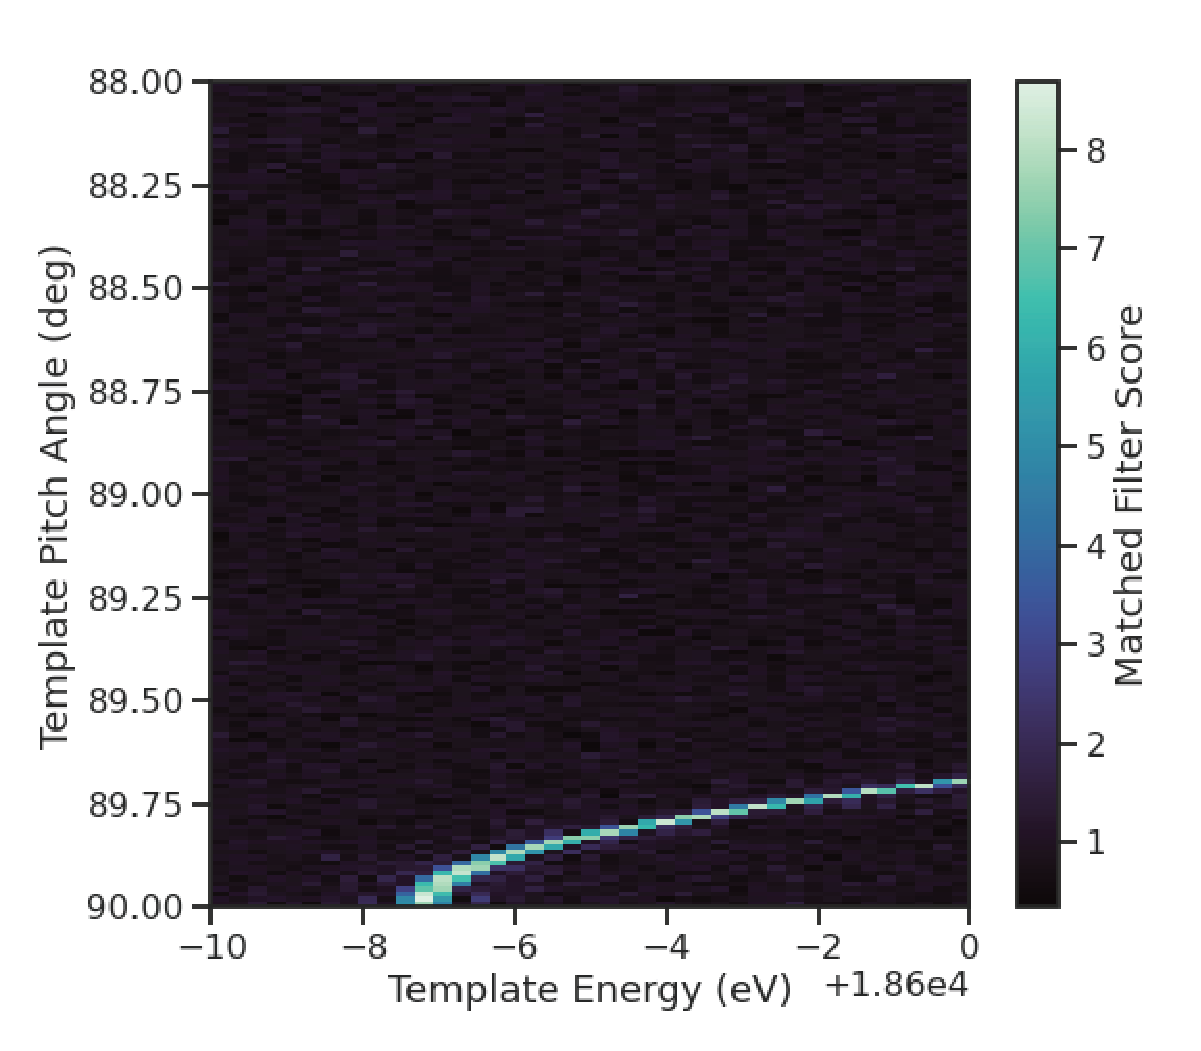
\includegraphics[width=\textwidth]{figs/Chapter-4/230517_mf_degen_1.png}
        \caption{}
    \end{subfigure}
    \hfill
    \begin{subfigure}{0.49\textwidth}
        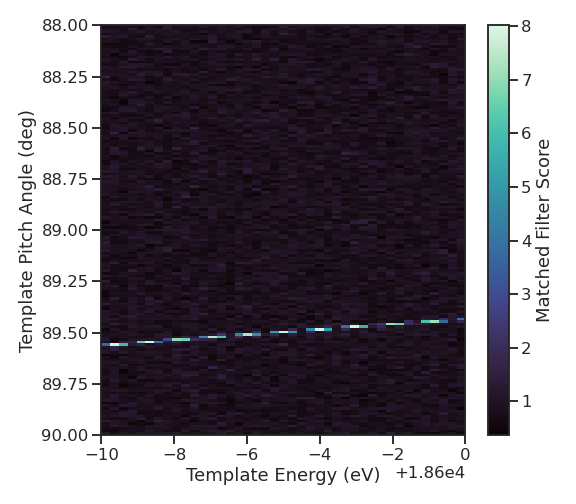
\includegraphics[width=\textwidth]{figs/Chapter-4/230517_mf_degen_2.png}
        \caption{}
    \end{subfigure}
    \caption{Two example illustrations of the correlation between kinetic energy and pitch angle imparted by the shape of the FSCD magnetic trap. The correlations manifest themselves as degeneracies in the matched filter score where multiple matched filter templates have the same matched filter for a particular signal. These degeneracies are a sign that the magnetic trap must be redesigned in order to break the correlation between pitch angle and kinetic energy. }
    \label{fig:chap4-mf-degeneracy}
\end{figure}

This degeneracy in matched filter score is the result of correlations between the kinetic energy of the electron and the pitch angle caused by changes in the average magnetic field experienced by an electron for different pitch angles. While in principle helpful for the purposes of signal detection these correlations are unacceptable since they greatly reduce the energy resolution of the experiment by causing electrons with specific kinetic energy to templates across a wide range of energies.
\begin{figure}[htbp]
    \centering
    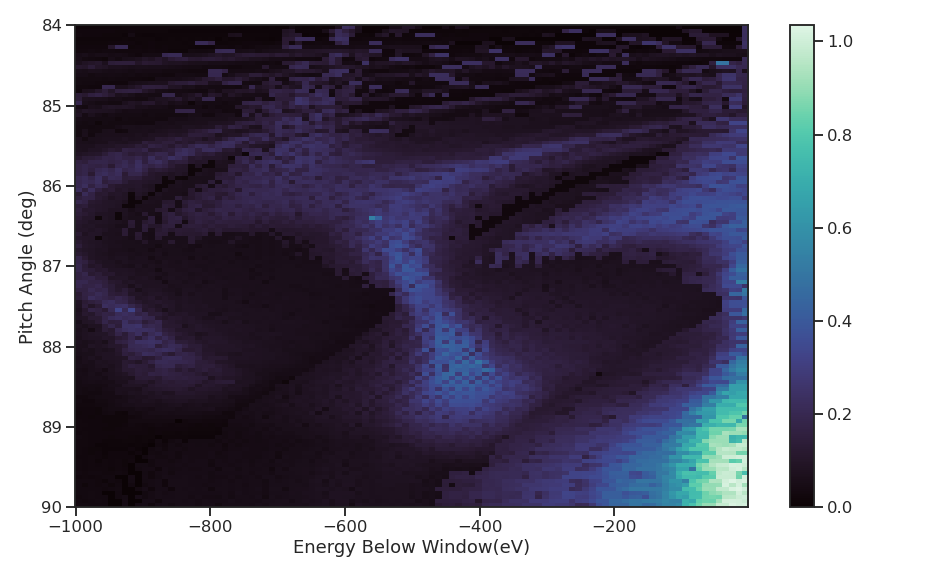
\includegraphics[width=0.7\textwidth]{figs/Chapter-4/230517_energy_pitch_correlation_map.png}
    \caption{A visualization of the correlation between energy and pitch angle in the FSCD magnetic trap. The image is formed by computing the match of the best template from a grid consisting of pitch angles from 84 to 90 degrees in steps of 0.05 degrees, kinetic energies from 17574 to 18574 eV, located at 2~cm from the central axis, and simulated for a length of three FSCD time-slices. The signals used to compute the best matching template consisted of a grid from 84 to 90 degrees in steps of 0.05 degrees, kinetic energies from 18550 to 18575 eV in steps of 0.25 eV, located 2~cm from the central axis, and simulated for three FSCD time-slices. The colored regions of the plot show how well signals with lower energy can match those of higher energy for the FSCD magnetic trap, which is proportional to the achievable energy resolution of the FSCD design.}
    \label{fig:chap4-mf-degeneracy-large-scale}
\end{figure}
It is important to emphasize that this degeneracy cannot be fixed by implementing a different signal reconstruction algorithm. As revealed by the matched filter scores the shapes of the signals for different parameters are identical. Resolving this degeneracy between pitch angle and energy requires the design of a new magnetic trap with steeper walls so that the average magnetic field experienced by an electron is less dependent on pitch angle.

\subsection{Machine Learning}

Machine learning is a vast and rapidly developing field of research \cite{prml}. In this Section we shall attempt to provided a brief introduction to some of the concepts and techniques of machine learning that were applied to CRES signal detection rather than attempt a comprehensive overview.

\subsubsection*{Introduction to Machine Learning}
\label{sec:chap4-intro-ml}

Digitization of the FSCD antenna array generates large amounts of data that must be rapidly processed to enable real-time signal detection and reconstruction. While digital beamforming combined with a power threshold is relatively computationally inexpensive, it is relatively ineffective at detecting CRES signal with small pitch angles, since it relies on a visible frequency peak above the noise. On the other hand, a matched filter is able to detect signals with a significantly larger range of parameters, however, the exhaustive search of matched filter templates can be computationally expensive. Machine learning based triggering algorithms have been used successfully in many different high-energy physics experiments \cite{ml_lhc} and recent developments have shown success in the detection of gravitational wave signals using machine learning techniques \cite{ml_ligo_1,ml_ligo_2} in place of the more traditional matched filtering method. This motivates the exploration of machine learning as a potential CRES signal detection algorithm. 

There are several different approaches to machine learning, but the one most important to our discussion here is the supervised learning approach. In supervised machine learning one uses a differentiable model or function that is designed to map the input data to the appropriate label \cite{prml}. The data is represented as a multidimensional matrix of floating point values such as an image or a time-series, and the label is generally a class name such as signal or noise for classification problems or a continuous value like kinetic energy in the case of regression problems. 

In supervised learning the model is trained to map from the data to the correct label by evaluating the output of the model using a training dataset consisting of a set of paired data and labels. To evaluate the difference between the model output and the correct label a loss function is used to quantify the error between the model prediction and the ground truth. For example, a common loss function in regression problems is the squared error loss function, which quantifies error using the squared difference between the model output and label. 

Using the outputs of the loss function the next step in supervised learning is to compute the gradient of error with respect to the model parameters in a process called backpropogation. Using the model parameter gradients the last step in the supervised learning process is to perform an update of the parameter values in order to minimize the error in the model predictions across the whole dataset. This loop is performed many times while randomly shuffling the dataset until the error converges to a minimum value at which point the training procedure has finished. It is standard practice to monitor the training procedure by evaluating the performance of the model using a separate validation dataset that matches the statistical distribution of the training data and to check the performance of the model after training using yet another dataset called the test dataset. These practices help to guard against overtraining which is a concern for models with many parameters.

\subsubsection*{Convolutional Neural Networks}

A popular class of machine learning models are neural networks. A neural network is essentially a function composed of a series of linear operations called layers which take a piece of data typically represented as a matrix, multiplies the elements of the data by a weight, and then sums these products to produce an output matrix. Neural networks composed of purely linear operations are unable to model complex non-linear behavior, therefore, non-linear activation functions are applied to the outputs of each of the layers to increase the ability of the neural network to model complex relationships between the data. 

Neural networks are typically composed of at least three layers, but with the present capabilities of computer hardware they more often contain many more than this. The first layer in a neural network is called the input layer, because it takes the data objects as input, and the last layer in a neural network is known as the output layer. The output layer is trained by machine learning to map the data to a desired output using the supervised learning procedure described in Section~\ref{sec:chap4-intro-ml}. In between the input and the output layer are typically several hidden layers that receive inputs from and transmit outputs to other layers in the neural network model. The term deep neural network (DNN) refers to those neural networks that have at least one hidden layer, which have proven to be extremely powerful tools for pattern recognition and function approximation.

An important type of DNN are convolutional neural networks (CNN) that typically contain several layers which perform a convolution of the input with a set of filters. These convolution operations are typically accompanied by layers that attempt to down-sample the data along with the standard neural network activation functions. A standard CNN is composed of several convolutional layers at the beginning of the network and ends with a series of fully-connected neural network layers at the output. Intuitively, one can imagine that the convolutional layers are extracting features from the data that fully-connected layers use to perform the classification or regression task.

\subsubsection*{Deep Filtering for Signal Detection in the FSCD}

\begin{figure}[htbp]
    \centering
    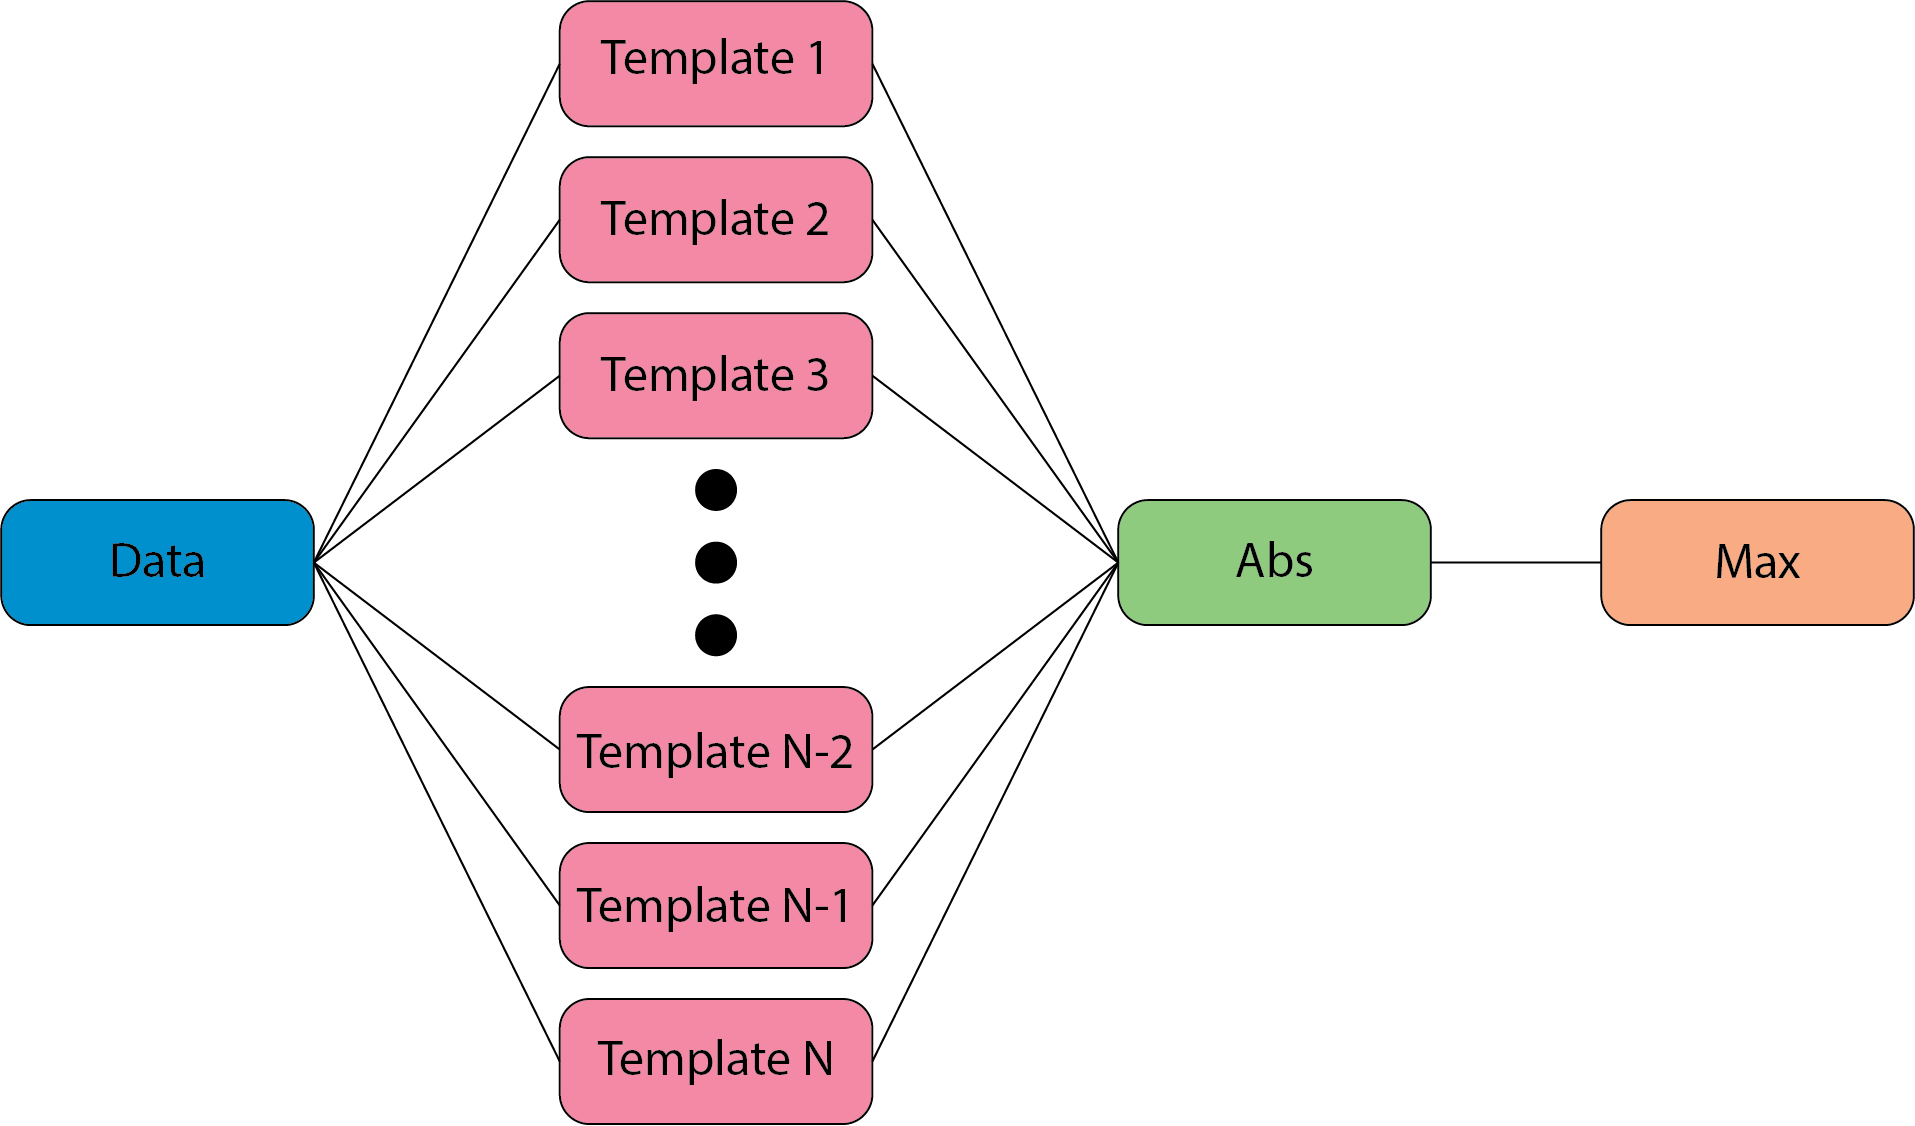
\includegraphics[width=0.66\textwidth]{figs/Chapter-4/230517_mf_conv_net.png}
    \caption{A representation of a matched filter template bank as a convolutional neural network. The network has a single layer composed of the templates, which act as convolutional filters. The activation of the neural network is an absolute value followed by a max operator.}
    \label{fig:chap4-mf-neural-network}
\end{figure}

CNNs have been extremely influential in the field of computer vision, particularly tasks such as image segmentation and classification, but have also been applied in numerous experimental physics contexts. Given the particular challenge posed by signal detection and reconstruction in the FSCD we are interested in exploring the potential of machine learning as an effective algorithm for real-time signal detection, since this application requires both high efficiency and fast evaluation.

In the machine learning paradigm signal detection is equivalent to a binary classification problem between the signal and noise data classes, and my investigation focuses specifically on the application of CNNs to signal detection in the FSCD, which is motivated by relatively recent demonstrations of CNNs achieving classification accuracies for gravitational wave time-series signals comparable to a matched filter template bank. In this framework it is possible to interpret the matched filter as a type of CNN composed of a single convolutional layer with the templates making up the layer filters (see Figure \ref{fig:chap4-mf-neural-network}). Since this neural network has no hidden layers, it is not a DNN like we have been discussing so far, but we can attempt to construct a proper CNN that attempts to reproduce the classification performance of the matched filter network.

The name deep filtering refers to this scheme of replacing a matched filter template bank with a DNN. The reason why one might want to do this is that it may be possible to exploit redundancies and correlations between templates that may allow one to perform signal detection with similar accuracy but with fewer computations, which is important for real-time detection scenarios like the FSCD experiment. In Section \ref{sec:chap4-trigger-paper} we perform a detailed comparison of the signal detection performance of a CNN to beamforming and a matched filter template bank.

Deep filtering is conceptually a simple technique. Similar to a matched filter template bank a large number of simulated CRES signals are generated and used to train a model to distinguish between signal and noise data (see Figure \ref{fig:chap4-deepfilter-process}). In order to reduce the dimensionality of the input FSCD data a digital beamforming summation is applied to the raw time-series data generated by Locust to compress the 60-channel data to a single time-series. CRES signal have a sparse frequency representation and experiments training CNN's on time-series and frequency series data found that models trained on frequency spectrum data performed significantly better, therefore, an FFT is applied to the summed time-series before being normalized and fed to the classification model.

%\begin{figure}[htbp]
%    \centering
%    \begin{subfigure}{0.55\textwidth}
%        \includegraphics*[width=\textwidth]{figs/Chapter-4/210604_training_info_dset_name210602_df1_ch3_temp10.0_modeldf_conv6_fc2_3ch_domain_freq.png}
%        \caption{}
%    \end{subfigure}
%    \begin{subfigure}{0.4\textwidth}
%        \includegraphics*[width=\textwidth]{figs/Chapter-4/210604_test_confusion_matrix_train_dset_210602_df1_ch3_test_dset_210602_df2_test_ch3_model_df_conv6_fc2_3ch_domain_freq_epoch_48.png}
%        \caption{}
%    \end{subfigure}
%    \caption{}
%\end{figure}

\begin{figure}[htbp]
    \centering
    \includegraphics*[width=0.9\textwidth]{figs/Chapter-4/230727_deep_filter_process.png}
    \caption{\label{fig:chap4-deepfilter-process} A graphical depiction of CRES signal detection using a CNN. A noisy segment of data is converted to a frequency series using digital beamforming and a FFT. The complex-valued frequency series is input into a trained CNN model that classifies the data as signal or noise using a decision threshold on the CNN output. }
\end{figure}

The data used to train the model consists of an equal proportion of signal and noise frequency spectra. Unique samples of WGN are generated and added to the signals during training time to avoid have to pre-generate and store large samples of noise data. The binary cross-entropy loss function combined with the ADAM optimizer proved effective at training the models to classify CRES data. A simple hyperparameter optimization was performed by manually tuning model, loss function, and optimizer parameters. The model and training loops was implemented in python using the PyTorch deep learning framework. Standard machine learning best practices were followed when training the models, such as overtraining monitoring using a validation dataset. Models were trained until the training loss and accuracy converged and then evaluated using a separate test data set.

\begin{figure}[htbp]
    \centering
    \includegraphics*[width=1.0\textwidth]{figs/Chapter-4/210625_plot_dfcnn_efficiency_vs_noise_temp.png}
    \caption{\label{fig:chap4-dfcnn-efficiency} The detection efficiency and false alarm rate (false positive rate) as a function of the decision threshold for different values of the noise temperature. The model is trained to output a value close to one for data that contains a signal and outputs a value near zero when the data contains only noise. One sees that a lower decision threshold will have a high detection efficiency at the cost of a high rate of false alarms. }
\end{figure}

The classification results of the test dataset are used to quantify the relationship between the true positive rate and the false positive rate for the model. The true positive rate is analogous to detection efficiency and the false positive rate is a potential source of background in the detector. One can limit the rate of false positives using a sufficiently high threshold on the model output at the cost of a lower detection efficiency (see Figure \ref{fig:chap4-dfcnn-efficiency} and Figure \ref{fig:chap4-dfcnn-roc}). As expected, the performance of the model at signal classification is negatively effected the noise power, which is quantified by the noise temperature.

\begin{figure}[htbp]
    \centering
    \includegraphics*[width=1.0\textwidth]{figs/Chapter-4/210625_plot_dfcnn_roc_vs_noise_temp.png}
    \caption{\label{fig:chap4-dfcnn-roc}ROC curves for a CNN model classifying CRES signals. One can see that the area under the curve, which is a figure of merit that descibes the performance of the classifier, is roughly linearly dependent with the noise temperature.}
\end{figure}

\clearpage


\section{Analysis of Signal Detection Algorithms for the Antenna Array Demonstrator}
\label{sec:chap4-trigger-paper}
This section contains an early version of the manuscript for the triggering paper prepared for publication in JINST. In it I present a relatively detailed analysis of the signal detection performance of the three signal detection approaches discussed so far using a population of simulated CRES signals generated with Locust. The focus of the paper is on the performance of the signal detection algorithms for pitch angles below $88.5^\circ$ where the beamforming power threshold begins to fail.

\subsection{Introduction}
Cyclotron Radiation Emission Spectroscopy (CRES) is a technique for measuring the kinetic energies of charged particles by observing the frequency of the cyclotron radiation that is emitted as they travel through a magnetic field \cite{p8originalcres}.
The Project 8 Collaboration is developing the CRES technique as a next-generation approach to tritium beta-decay endpoint spectroscopy for neutrino mass measurement. Recently, Project 8 has used CRES to perform the first ever tritium beta-decay energy spectrum and neutrino mass measurement \cite{p8prl2023, p8prc2023}.

Previous CRES measurements have utilized relatively small volumes of gas that are directly integrated with a waveguide transmission line, which transmits the cyclotron radiation emitted by the trapped electrons to a cryogenic amplifier. While this technology has had demonstrable success, it is not a feasible option for scaling up to significantly larger measurement volumes. In particular, the goal of the Project 8 Collaboration is to use CRES combined with atomic tritium to measure the neutrino mass with a 40~meV sensitivity. Achieving this sensitivity goal will require a multi-cubic-meter scale measurement volume in order to obtain the required event statistics in the tritium beta-spectrum endpoint region; hence, there is a need for new techniques to enable large volume CRES measurements for future experiments.

One approach is to surround a large volume with an array of antennas that together collect the cyclotron radiation emitted by trapped electrons \cite{p8snowmass2022, p8PanicProc}. A promising array design is an inward-facing uniform cylindrical array that surrounds the tritium containment volume. Increasing the size of the antenna array, by adding additional rings of antennas along vertical axis, allows one to grow the experimental volume until a sufficient amount of tritium gas can be observed by the array. A challenging aspect of this approach is that the total radiated power emitted by an electron near the tritium spectrum endpoint is on the order of 1~fW or less, which is then distributed between all the antennas in the array. Consequently, detecting the presence of a CRES signal and determining the electron's kinetic energy requires reconstructing the entire antenna array output over the course of the CRES event, posing a significant data acquisition and signal reconstruction challenge.

Project 8 has developed a triggering system to enable real-time identification of CRES events using an antenna array \cite{p8daqIII}. Previous measurements with the CRES technique have utilized a threshold on the frequency spectrum formed from a segment of CRES time-series data. This algorithm relies on the detection of a frequency peak above the thermal noise background, which limits the kinematic parameter space of detectable electrons. Due to the limitations of this power threshold, Project 8 has been investigating alternative signal identification approaches, including both matched filtering and machine learning based classifiers, to improve the detection efficiency of the experiment. In order to evaluate the relative gains in detection efficiency that come from utilizing these alternative algorithms, we develop analytical models for the power threshold and matched filter signal classifier performance applicable to an antenna array based CRES detector. In addition, we implement and test a basic convolutional neural network (CNN) as a first step towards the development of neural-network based classifiers for CRES measurements. These results allow us to compare the estimated detection efficiencies of each of these methods, which we weigh against the associated computational costs for real-time applications.

The outline of this paper is as follows. In Section \ref{sec:real-time-triggering} we give an overview of a prototypical antenna array CRES experiment, and describe the major steps involved in the proposed approach to real-time signal identification. In Section \ref{sec:classifiers} we develop models for the power threshold and matched filter algorithms, and introduce the machine learning approach and CNN architecture. In Section \ref{sec:method} we describe our process for generating simulated CRES signal data and the details of training the CNN. Finally, in Section \ref{sec:results} we perform a comparison of the signal classification accuracy of the three approaches and discuss the relevant trade-offs in terms of detection efficiency and computational cost.

\begin{figure}[h]
    \centering
    \begin{subfigure}{0.48\textwidth}
        \centering
        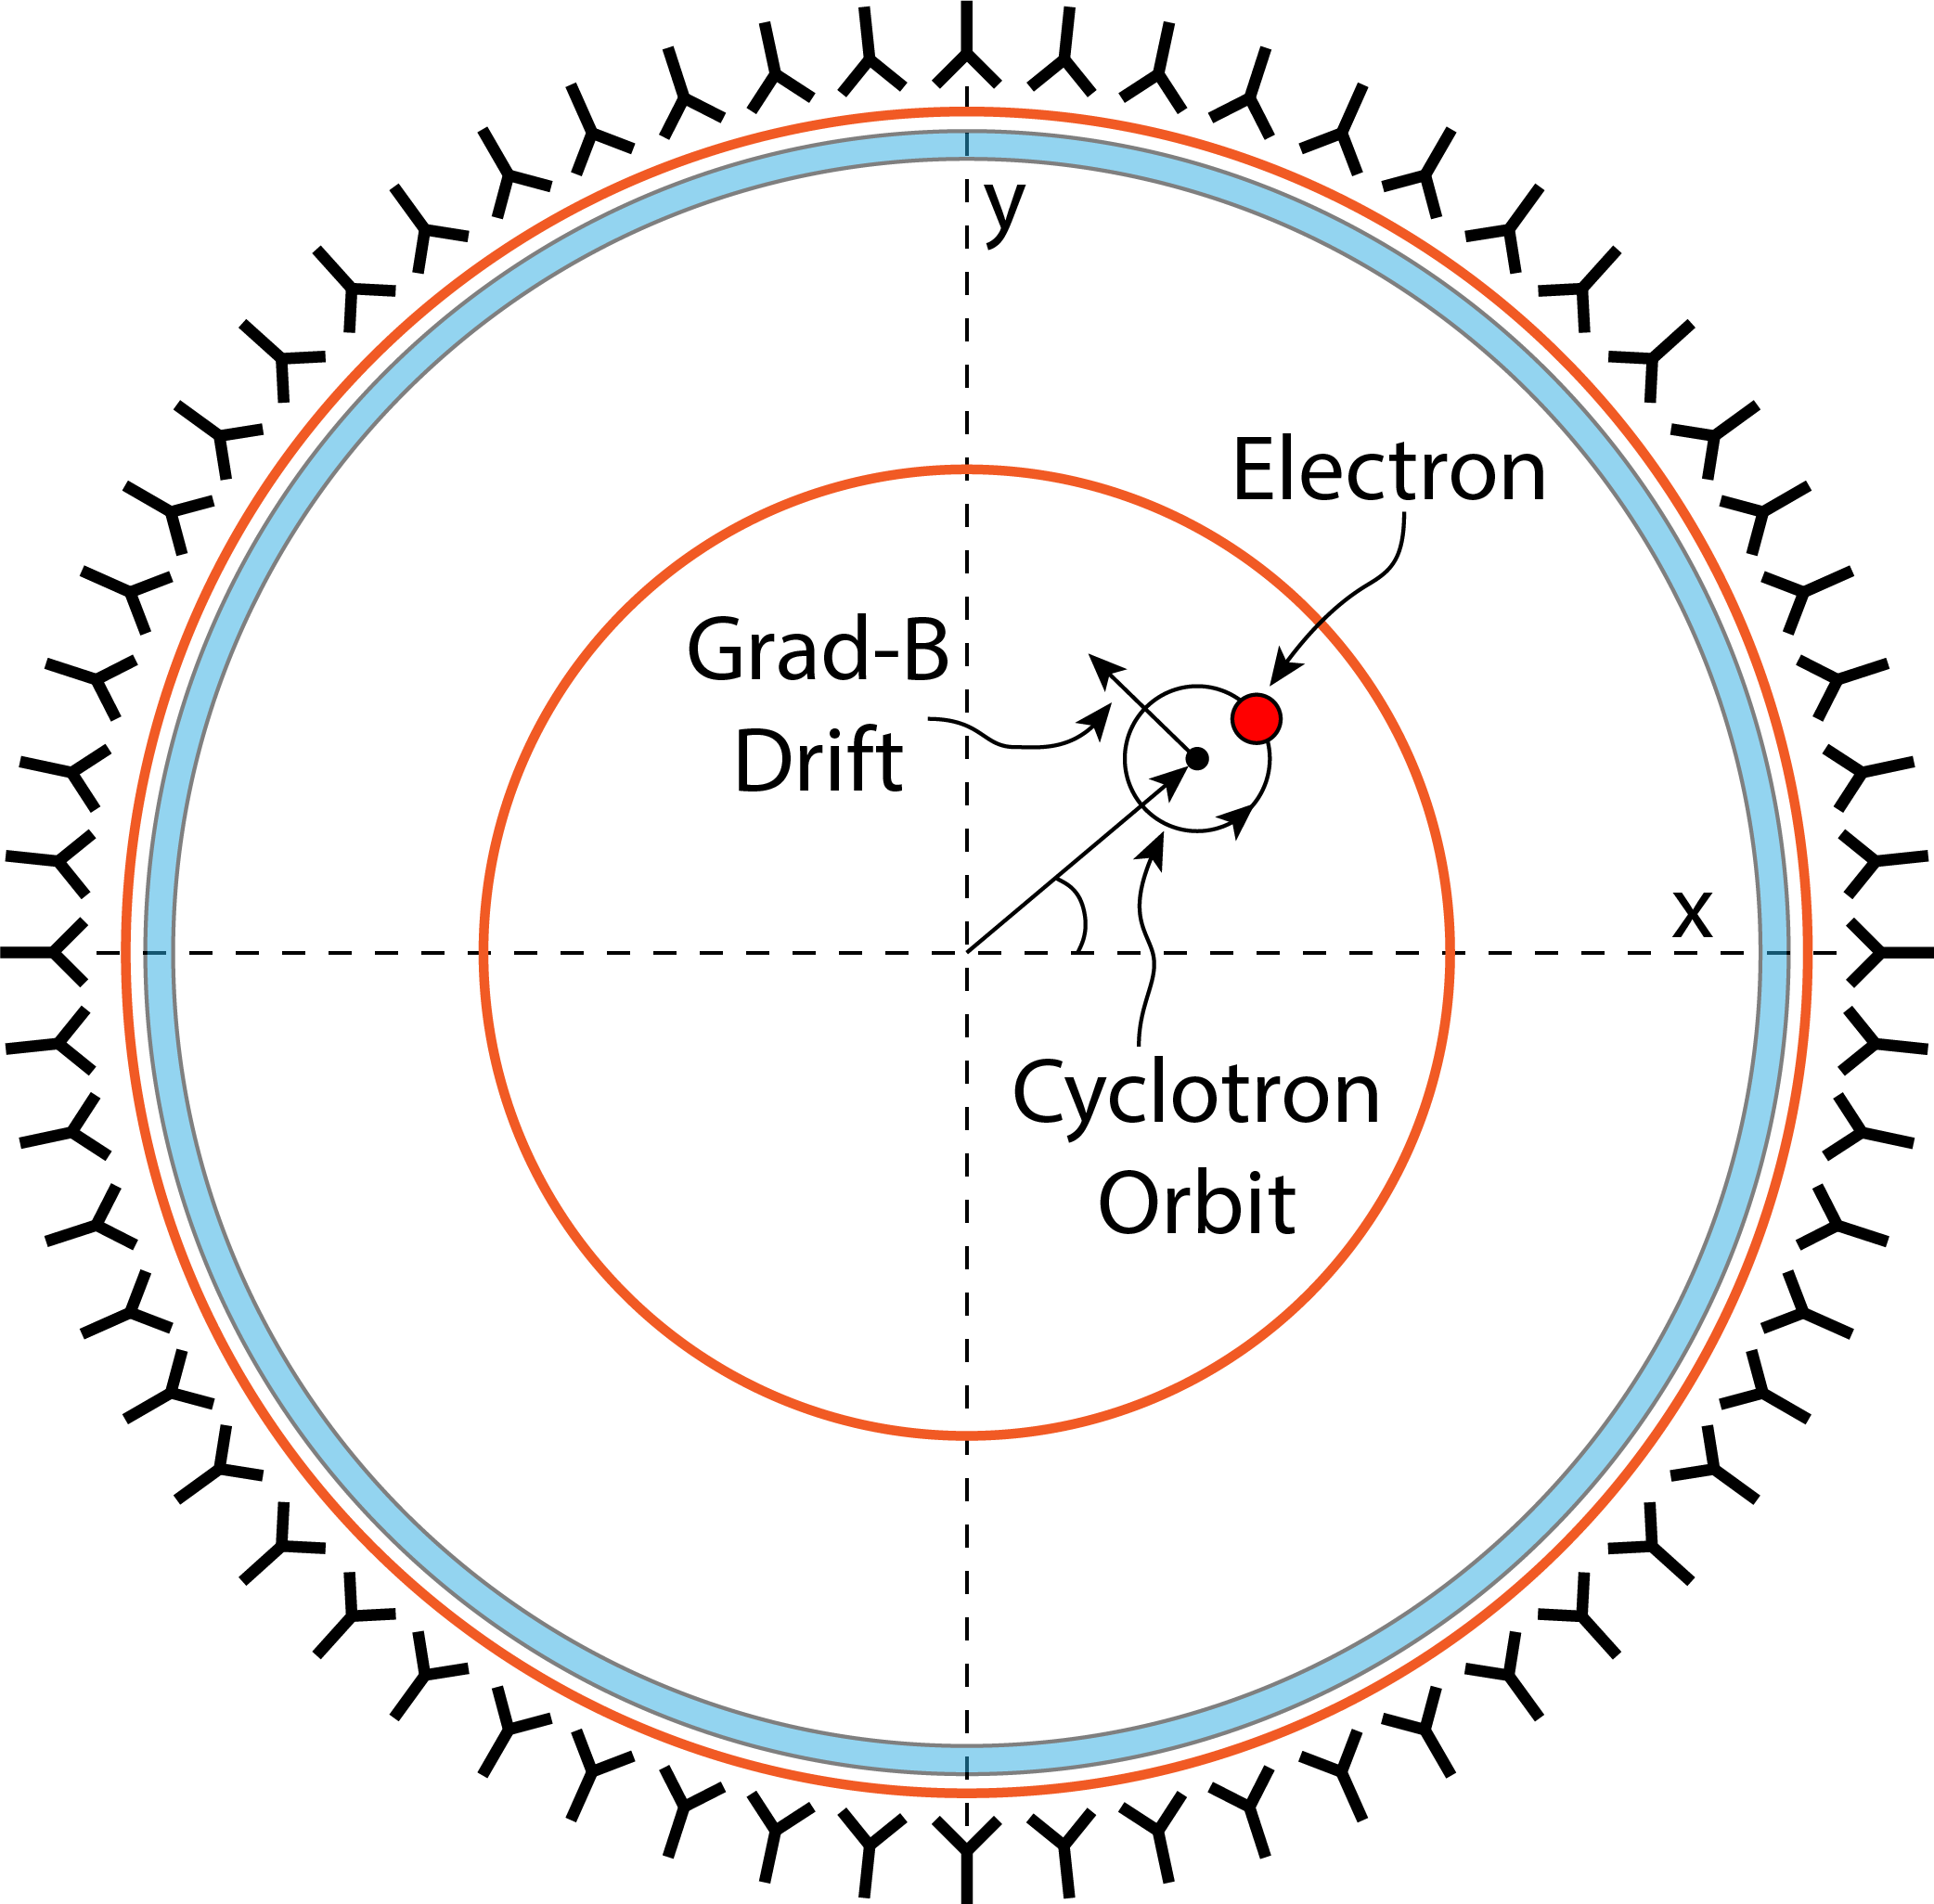
\includegraphics[width=0.9\textwidth]{figs/Chapter-4/230328_deepfilter_paper_apparatus_concept_top_v2.png}
        \caption{Top-down view.}
        \label{fig:apparatus_concept_top}
    \end{subfigure}
    \begin{subfigure}{0.48\textwidth}
        \centering
        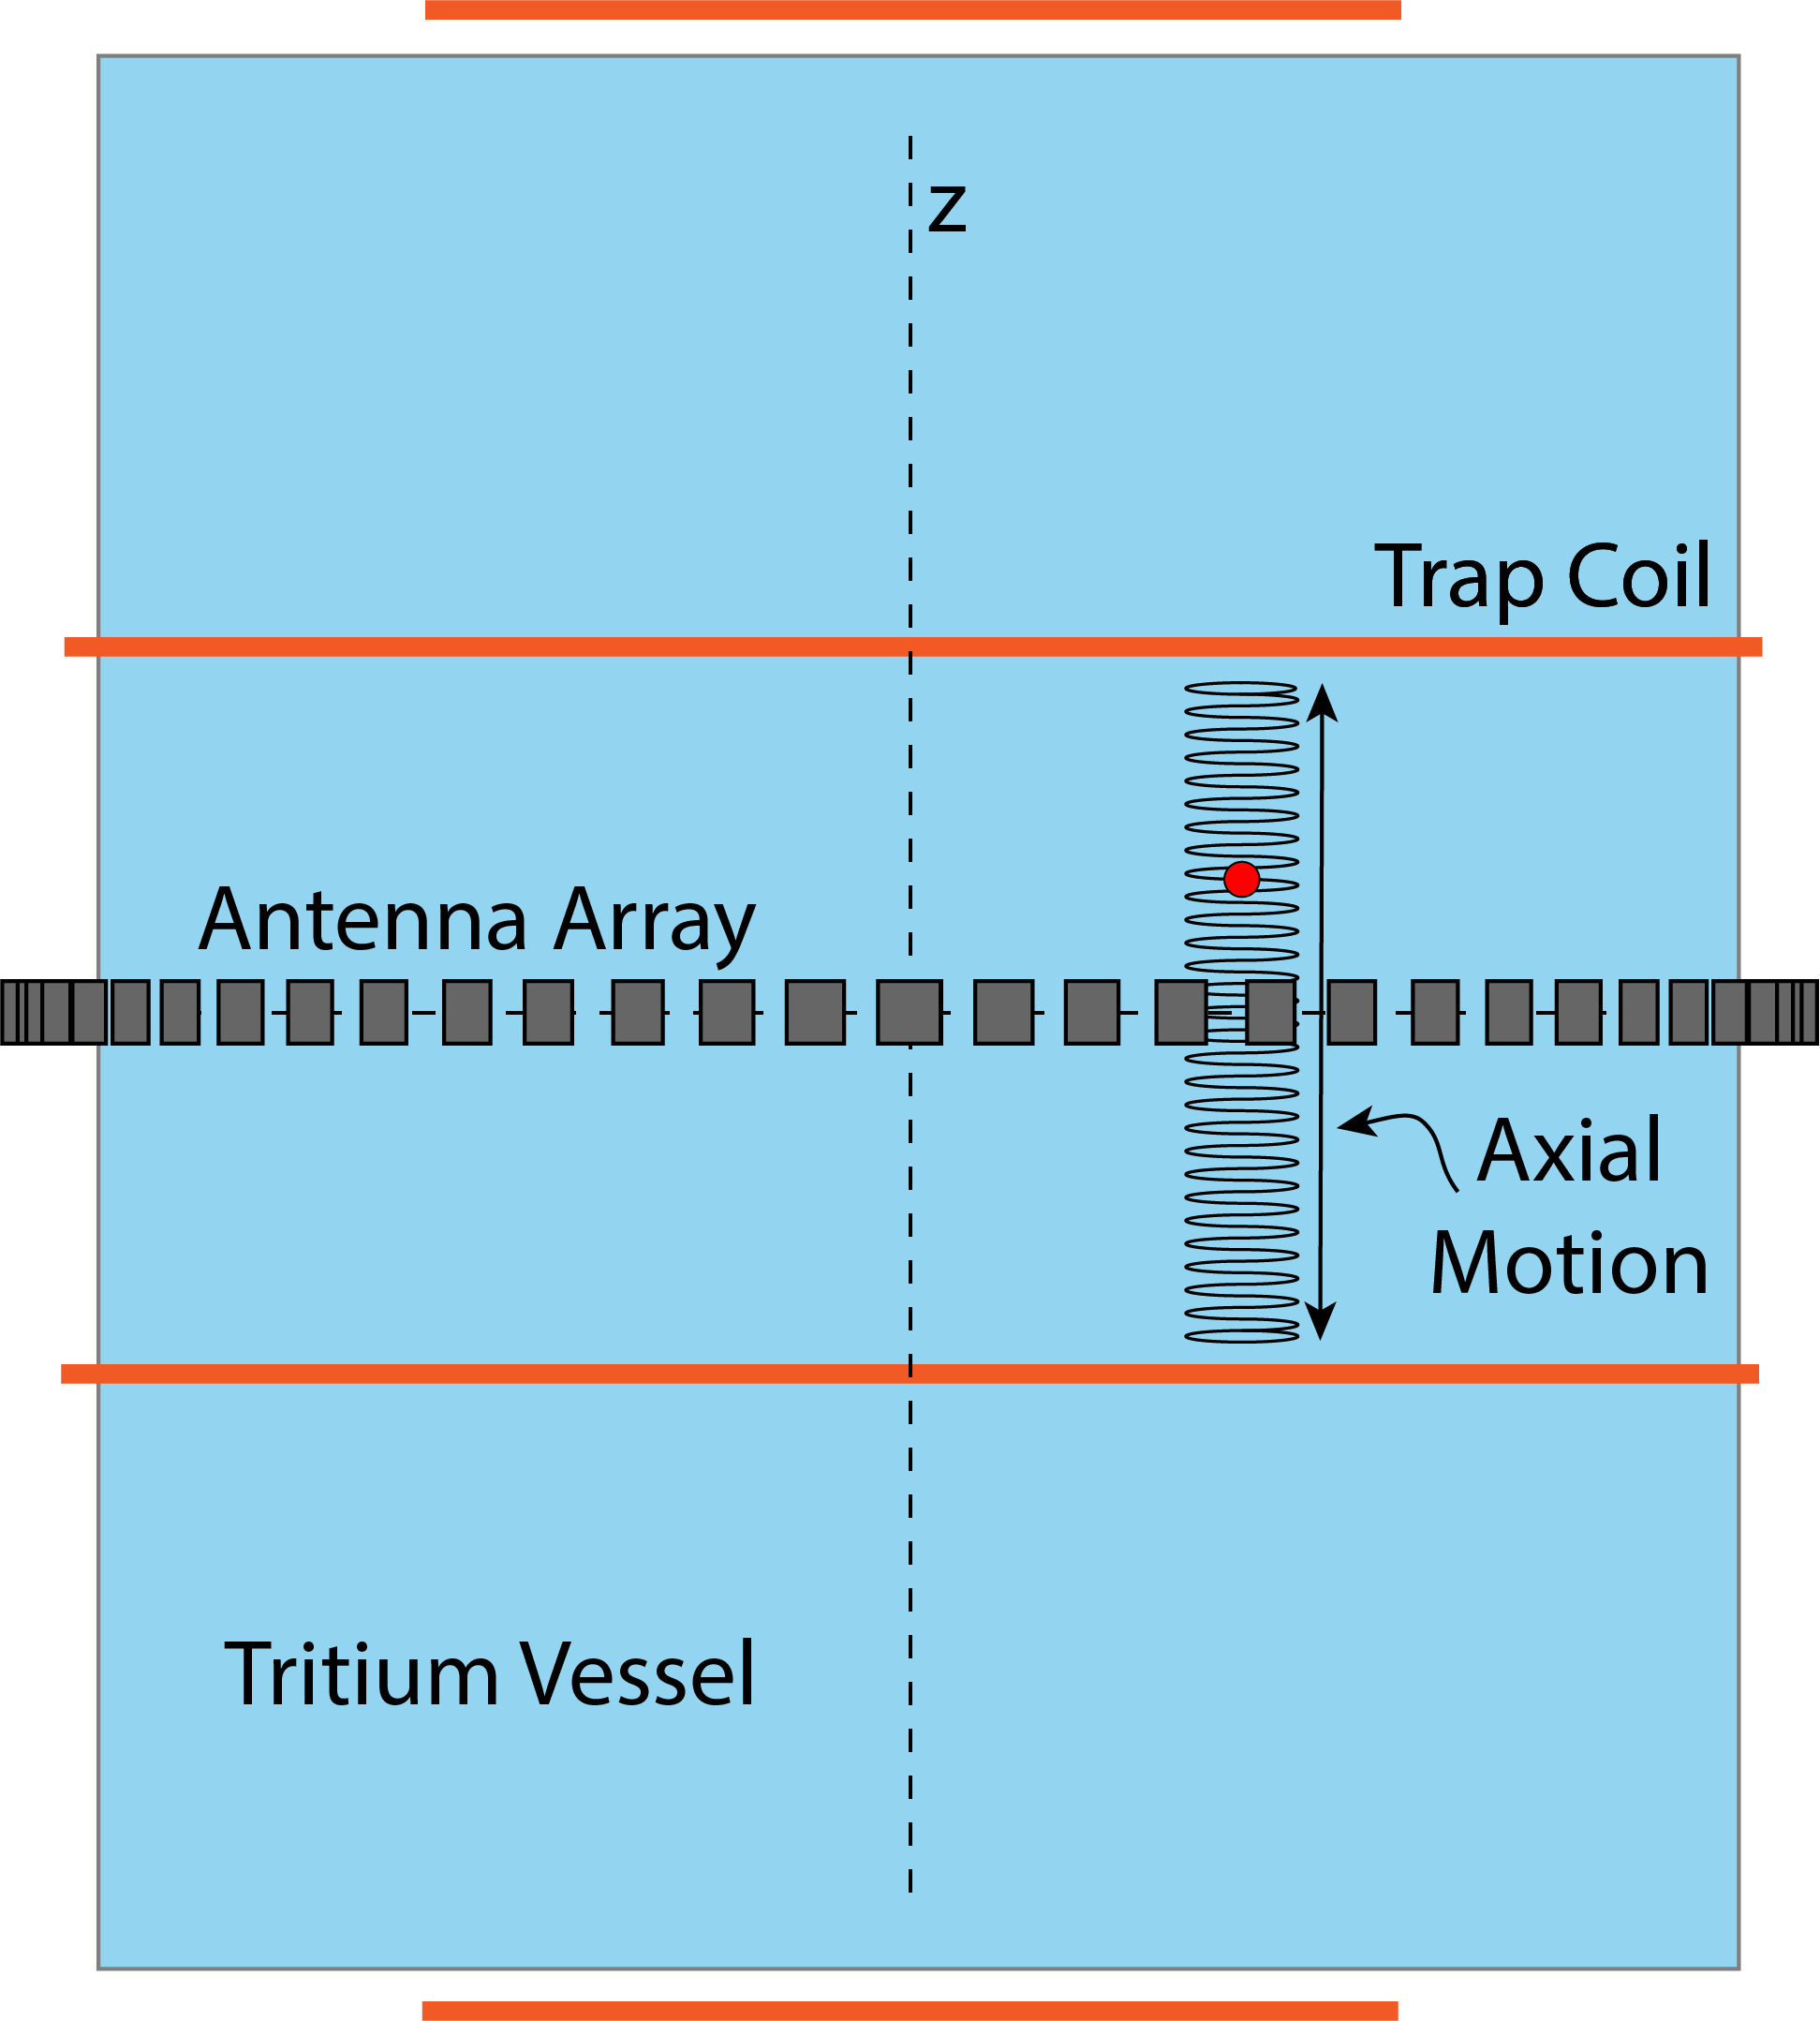
\includegraphics[width=0.8\textwidth]{figs/Chapter-4/230328_deepfilter_paper_apparatus_concept_side_v2.png}
        \caption{Side view.}
        \label{fig:apparatus_concept_side}
    \end{subfigure}
    \caption{An illustration of the conceptual design for an antenna array CRES tritium beta-decay spectrum measurement. The antenna array geometry consists of a 20~cm interior diameter with 60 independent antenna channels arranged evenly around the circumference. The nominal antenna design is sensitive to radiation in the frequency range of 25-26~GHz, which corresponds to the cyclotron frequency of electrons emitted near the tritum beta-spectrum endpoint in a 1~T magnetic field. The array is located at the center of the magnetic trap produced by a set of current-carrying coils. The nominal magnetic trap design is capable of trapping electrons up to 5~cm away from the central axis of the array and traps electrons within an approximately 6~cm long axial region centered on the antenna array.}
    \label{fig:apparatus_concept}
\end{figure}


\subsection{Signal Detection with Antenna Array CRES}
\label{sec:real-time-triggering}


\subsubsection{Antenna Array and DAQ System}
\label{sec:aa-and-daq}

In order to explore the potential of antenna array CRES for neutrino mass measurement, the Project 8 Collaboration has developed a conceptual design for a prototype antenna array CRES experiment \cite{p8PanicProc,p8snowmass2022}, called the Free-space CRES Demonstrator or FSCD, which could be used as a demonstration of the antenna array measurement technique (see Figure \ref{fig:apparatus_concept}). The FSCD utilizes a single ring of antennas, which is the simplest form of a uniform cylindrical array configuration, to surround a radio-frequency (RF) transparent tritium gas vessel. A prototype version of this antenna array has been built and tested by the Project 8 collaboration to validate simulations of the array radiation pattern and beamforming algorithms \cite{p8jugaad}. In the FSCD the antenna array is positioned at the center of the magnetic trap formed by a set of electro-magnetic coils that are designed to produce a magnetic trap with flat central region and steep walls both radially and axially. 

When a beta-decay electron is trapped its motion consists of three primary components. The component with the highest frequency is the cyclotron orbit whose frequency is determined by the size of the background magnetic field. The FSCD design assumes a background magnetic field value of approximately 0.96~T, which results in cyclotron frequencies for electrons with kinetic energies near the tritium beta-spectrum endpoint from 25 to 26~GHz. The component with the next highest frequency is the axial oscillation experienced by electrons with pitch angles of less than $90^\circ$ \cite{p8pheno}. The flat region of the FSCD magnetic trap extends approximately 3~cm above and below the antenna array plane causing electrons to move back and forth as they are reflected from the trap walls. Typical oscillation frequencies are on the order of ~10's of MHz, which results in an oscillation period that is $O(10^3)$ smaller than the duration of a typical CRES event. Therefore, when reconstructing CRES events we treat the electron as occupying only an average axial position at the center of the magnetic trap, since we are not able to resolve the axial position as a function of time. The component of motion with the smallest frequency is $\nabla B$-drift caused by radial field gradients in the trap, producing an orbit of the electron around the central axis of the trap with a frequency on the order of a few kHz, dependent on the pitch angle and the radial position of the electron. 

\begin{figure}[htbp]
    \centering
    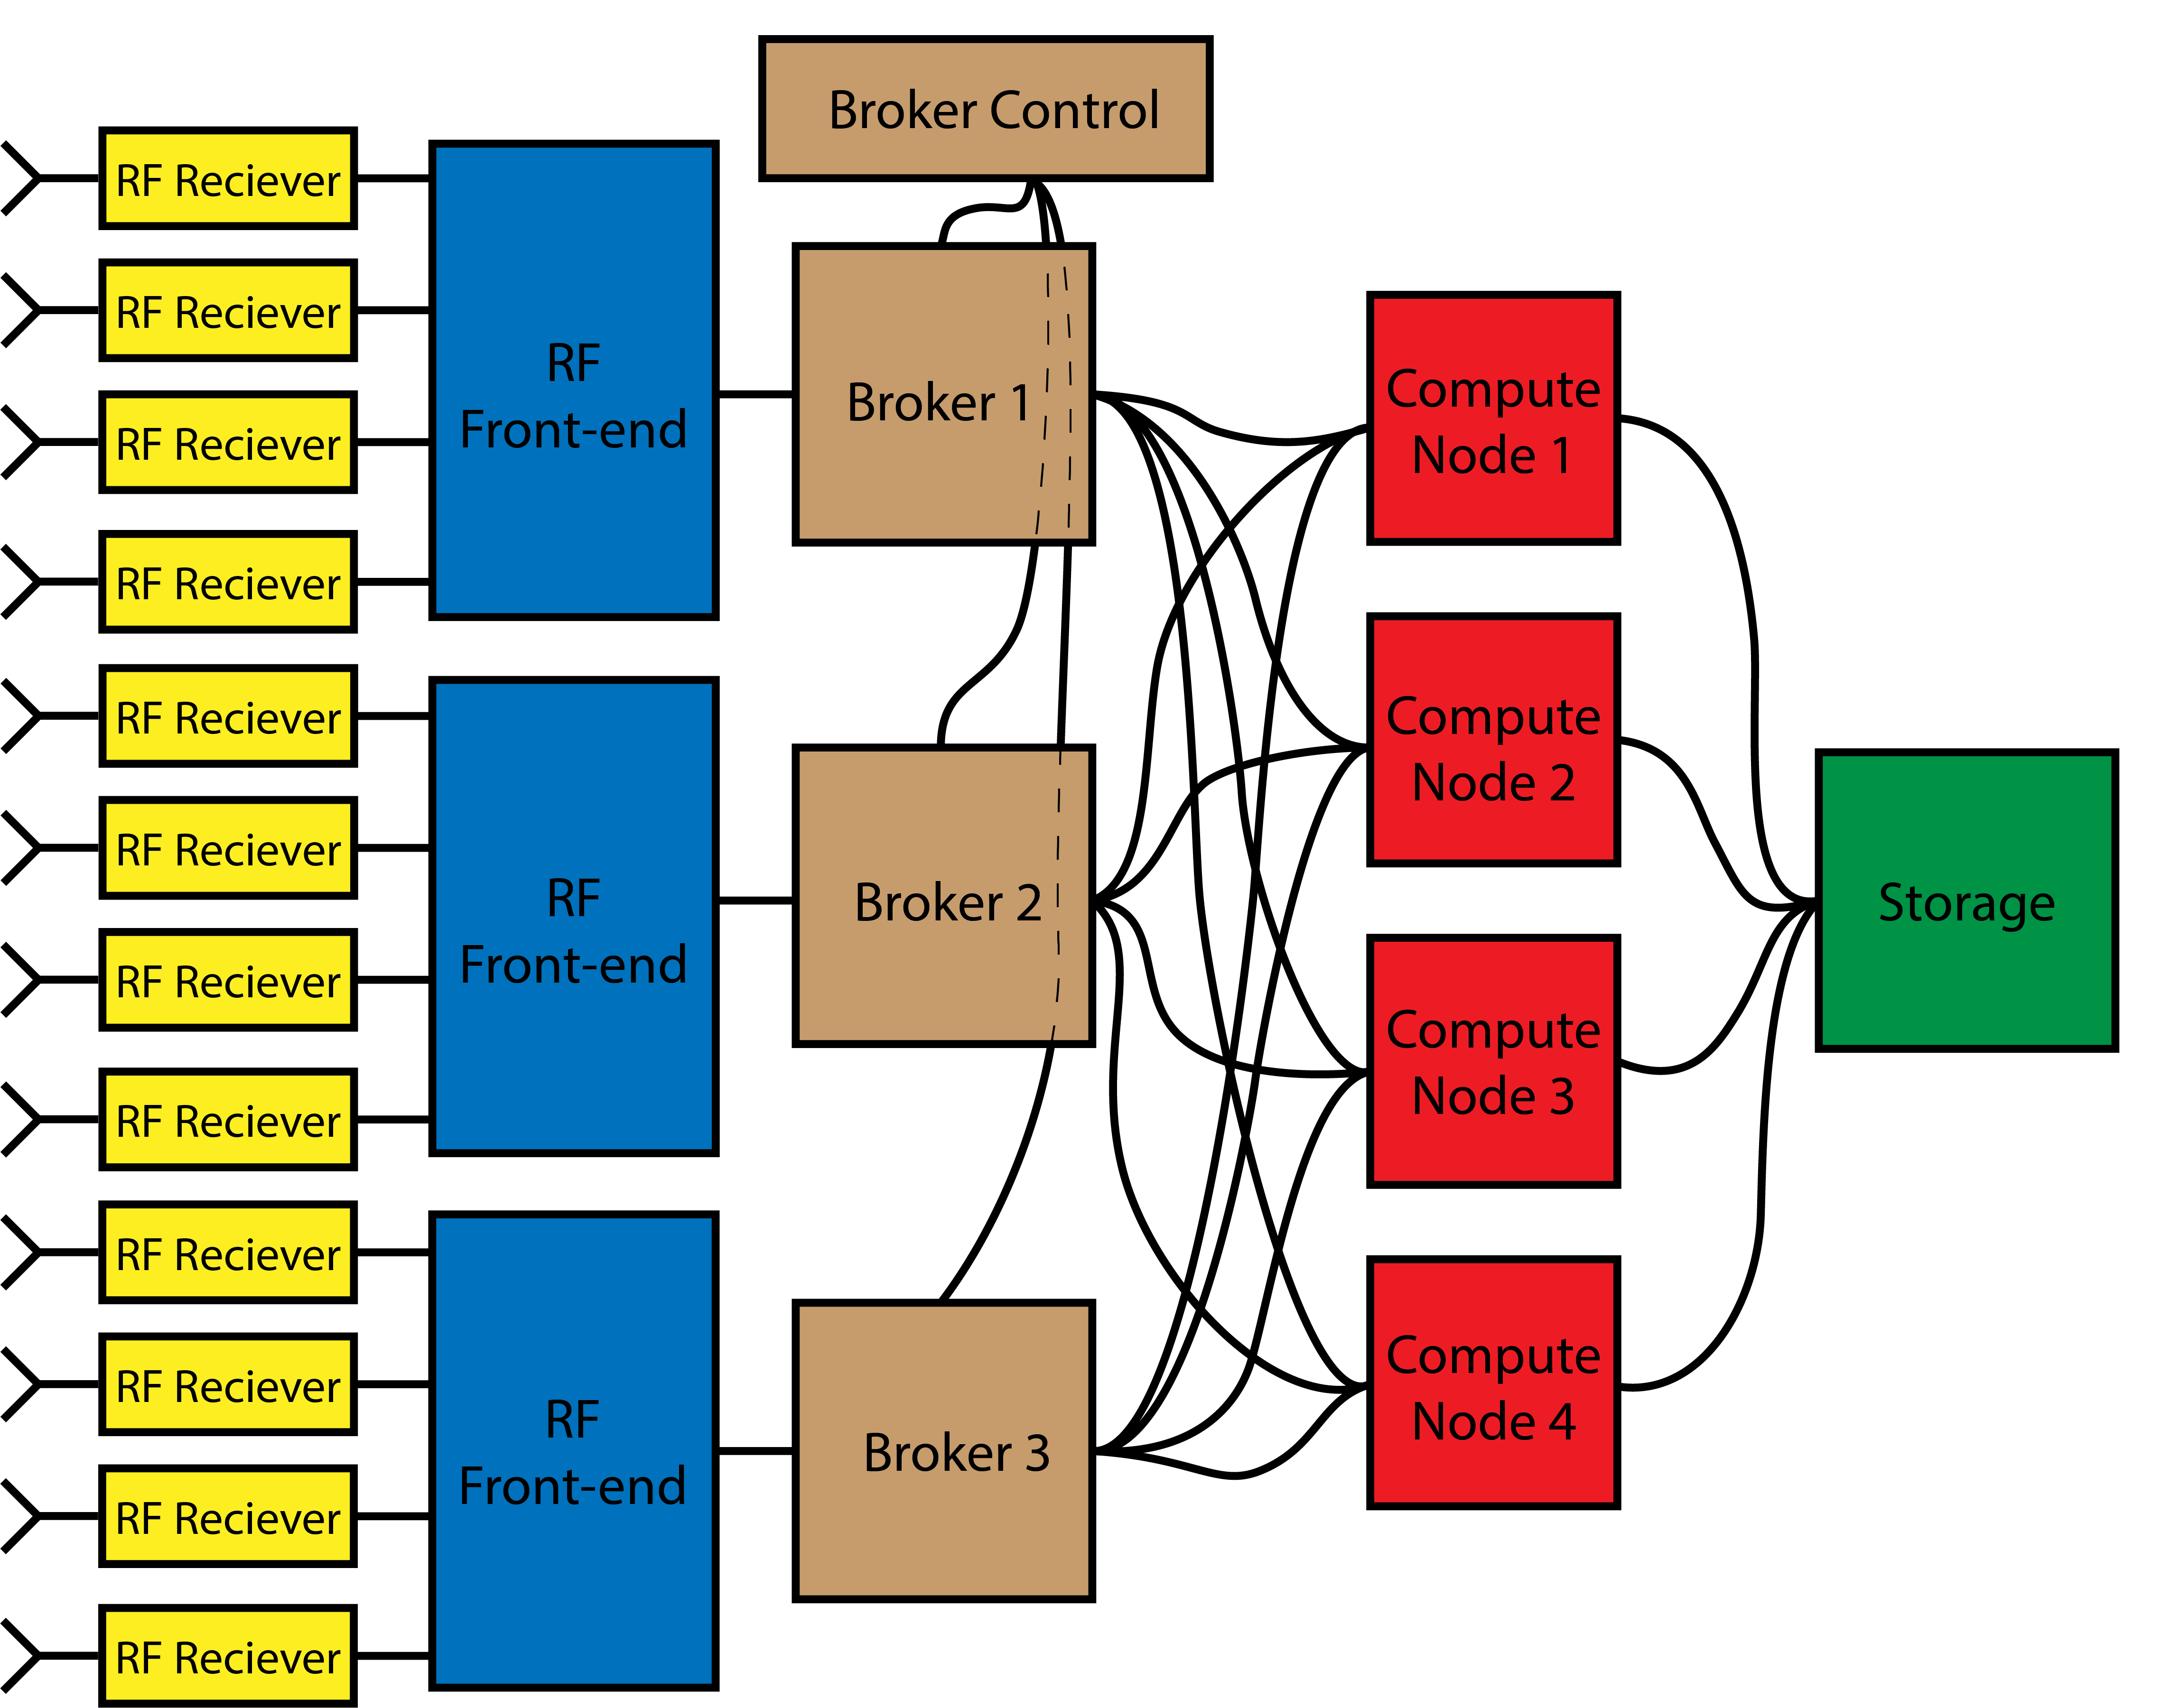
\includegraphics[width=0.5\textwidth]{figs/Chapter-4/230108_daq_system_overview.png}
    \caption{A high-level diagram of the DAQ system archtecture envisioned for the FSCD.}
    \label{fig:chap4-daq-system-overview}
\end{figure}

The data acquisition (DAQ) system digitizes the signals from the antenna array and combines thee data streams into a time-ordered matrix of array snapshots that can be used by the reconstruction algorithms. The FSCD DAQ system design \cite{p8daqIII} is divided into three layers \ref{fig:chap4-daq-system-overview}. The first layer is the RF front-end, which includes the antenna array, the RF receiver boards, and the digitization electronics. The receiver board contains an amplifier, RF mixer, and bandpass filter to enable down-conversion, and is followed by the digitization electronics that sample the CRES signals at 200~MHz. In order to achieve an adequate signal-to-noise ratio to detect CRES events, the DAQ system for the antenna array demonstrator must have a total system noise temperature of $\approx 10$~K, which we can achieve by using low-noise amplifiers and operating at cryogenic temperatures. After digitization, the array data must be reorganized from individual data streams sorted by channel into array snapshots sorted by time. In order to solve this data transfer and networking problem the second layer of the DAQ system consists of a set of broker computer nodes that reorganize the array data into time-ordered chunks. This approach allows us accommodate different data transfer requirements by scaling the number of broker nodes in this layer accordingly. Next, the broker layer distributes these chunks of array data to the final layer of the DAQ system, which consists of a set of identical reconstruction nodes that perform the calculations required for CRES reconstruction. Similar to the broker layer, the number of reconstruction nodes can be increased or decreased depending on the amount of computer power required for real-time CRES reconstruction.


\begin{figure}[htbp]
    \centering
    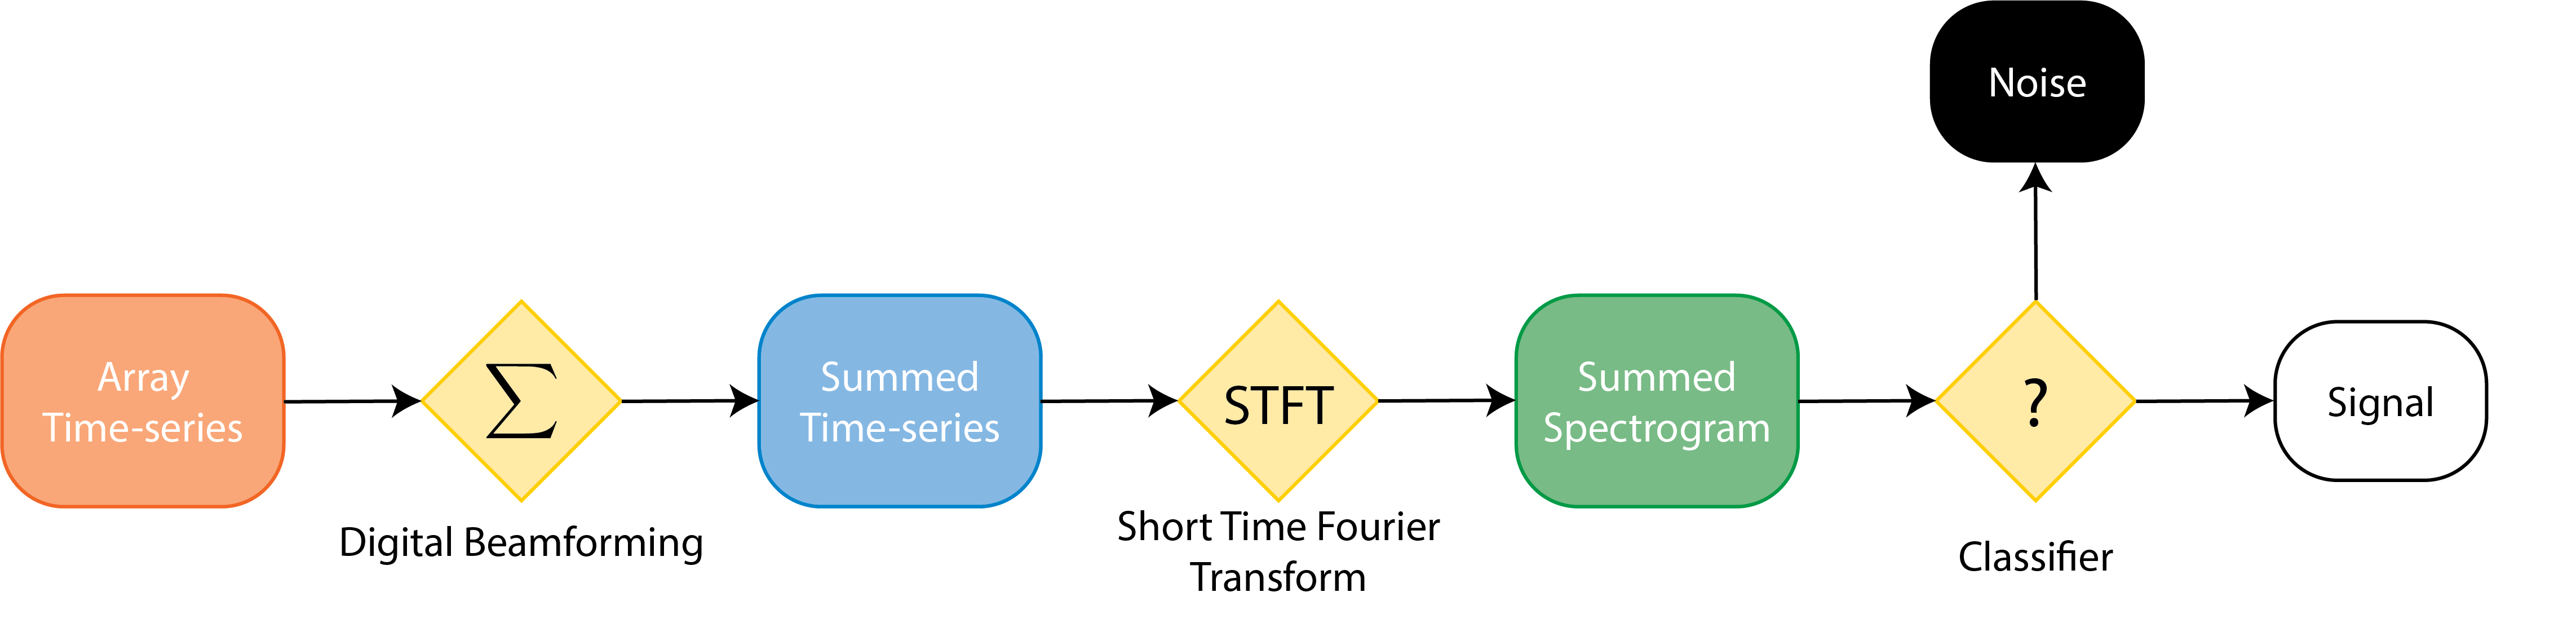
\includegraphics[width=0.9\textwidth]{figs/Chapter-4/230316_trigger_flowchart.png}
    \caption{A block diagram illustration of the real-time triggering algorithm proposed for antenna array CRES reconstruction.}
    \label{fig:signal_detection_routine}
\end{figure}

The design of the FSCD DAQ system is intended to enable a significant portion of the CRES event reconstruction to occur in real-time. The motivation for this comes from the fact that the FSCD antenna array generates approximately 1~exabyte of raw data per year of operation. Therefore, in order to reduce the data-storage requirements, it is ideal to perform at least some of the CRES event reconstruction in real-time so that it is possible to save a reduced form of the data for offline analysis. The first step of the real-time reconstruction would be a real-time signal detection algorithm, which is the focus of this paper. Our approach consists of three main operations performed on the time-series data blocks including digital beamforming, a short time Fourier transform (STFT), and a binary classification algorithm to distinguish between signal and noise data (see Figure \ref{fig:signal_detection_routine}). 

\subsubsection{Real-time Signal Detection}
\label{sec:bf-and-stft}

\begin{figure}[htbp]
    \centering
    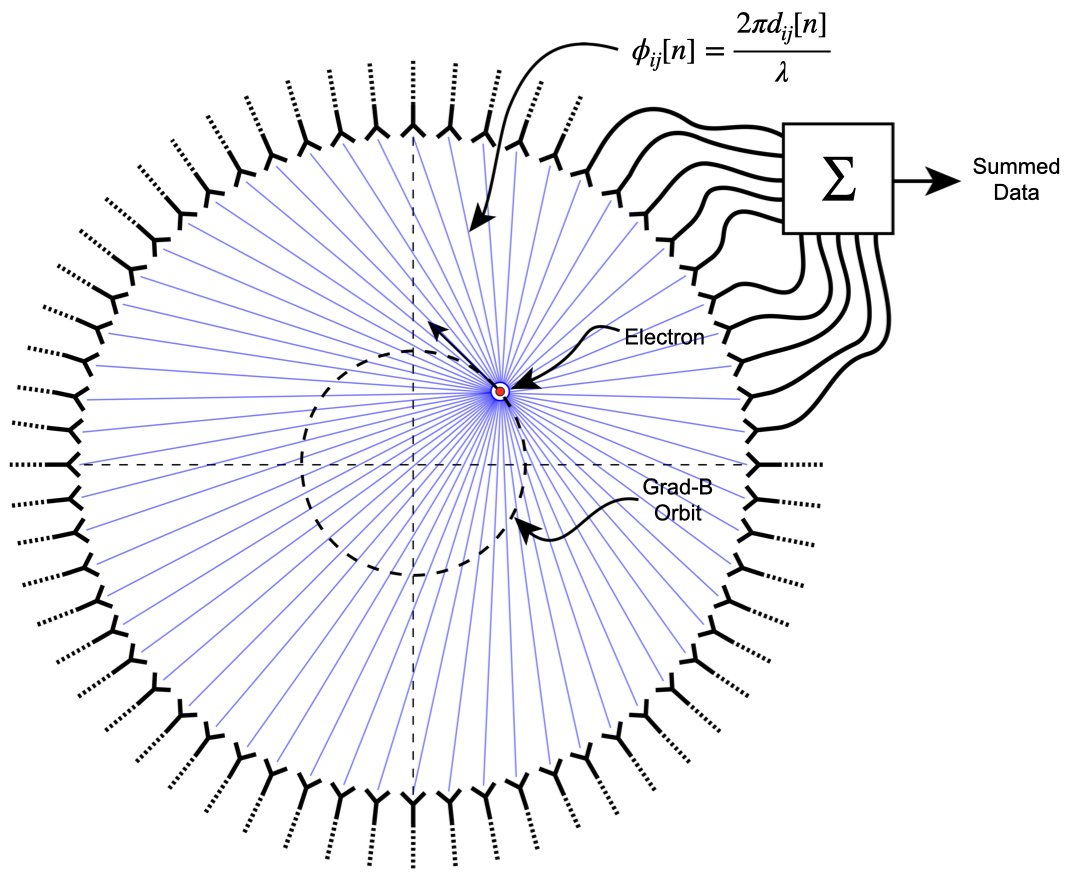
\includegraphics[width=0.65\textwidth]{figs/Chapter-4/230216_beamforming_diagram_annotated.001.png}
    \caption{An illustration of the digital beamforming procedure. The blue lines indicate the various distances from the beamforming position to the antenna. In the situation depicted the actual position of the electron matches the beamforming position, so we should expect constructive interference when the phase shifted signals are summed. To prevent the electron's $\nabla B$-motion from moving the electron off of the beamforming position, the beamforming phase include a time-dependence to follow the trajectory of the electron in the magnetic trap.}
    \label{fig:beamforming}
\end{figure}

The first step in the real-time detection algorithm is digital beamforming, which is a phased summation of the signals received by individual antennas in the array (see Figure \ref{fig:beamforming}). The phase shifts correspond to the path length differences between a spatial position and each individual antenna such that, when there is an electron located at the beamforming position, all the signals received by the array constructively interfere. Since we do not know ahead of time where an electron will be produced in the detector, we define a grid of beamforming positions that cover the entire region where electrons can be trapped and perform a phased summation for each of these points for every time-step in the array data block. As we saw in Section \ref{sec:aa-and-daq}, the axial oscillation of the electrons prevents us from resolving it's position along the Z-axis of the trap, therefore our beamforming grid need only cover the possible positions of the electron in the two-dimensional plane defined by the antenna array. 

The equation defining digital beamforming can be expressed as
\begin{equation}
    \mathbf{y}[n] = \mathbf{\Phi}^T[n]\mathbf{x}[n],
    \label{eq:beamforming}
\end{equation}
where $\mathbf{x}[n]$ is array snapshot vector at the sampled time $n$, $\mathbf{\Phi}[n]$ is the matrix of beamforming phase shifts, and $\mathbf{y}[n]$ is summed output vector that contains the voltages for each of the summed channels that correspond to a particular beamforming position. % For each time sample in the array data matrix, we perform $N_b$ different phased summations where $N_b$ is the number of beamforming positions. 
The elements of the beamforming phase shift matrix can be expressed as a weighted complex exponential
\begin{equation}
    \mathbf{\Phi}_{ij}[n]=A_{ij}[n]\exp{\left(2\pi i\phi_{ij}[n]\right)},
\end{equation}
where the indices $i$ and $j$ label the beamforming and antenna positions respectively. The weight $A_{ij}$ accounts for the relative power increase for antennas that are closer to the position of the electron, and $\phi_{ij}$ is the total beamforming phase shift for the $j$-th antenna at the $i$-th beamforming position.

The beamforming phase shift is a sum of two terms
\begin{equation}
    \phi_{ij}[n]=\frac{2\pi d_{ij}[n]}{\lambda}+\theta_{ij}[n],
\end{equation}
where the first term is the phase shift originating from the path length difference ($d_{ij}[n]$) between the beamforming and antenna positions, which are represented by the vectors $(r_j,\theta_j)$ and $(r_i,\theta_i[n])$, and the second term is the angular separation ($\theta_{ij}[n]$) of the two positions. The angular separation enters into the beamforming phase due to an effect caused by the circular orbit of the electron that produces radiation whose phase is linearly dependent on the relative azimuthal position of the antenna \cite{nb_thesis, p8synca}. The time-dependence of the beamforming phases is intended to correct for the effects of $\nabla B$-drift, which cause the guiding centers of electrons to orbit the center of the magnetic trap. By including a linear time-dependence in the azimuthal beamforming position,
\begin{equation}
    \theta_{i}[n]=\omega_{\nabla B}t[n]+\theta_{i,0},
\end{equation}
where $\omega_{\nabla B}$ is the azimuthal grad-B drift frequency, $t[n]$ is the time vector and, $\theta_{i,0}$ is the starting azimuthal position, we can configure the beamforming phases to effectively track the XY-position of the guiding center over the event duration. Predicting accurate values of $\omega_{\nabla B}$ for a specific trap and set of kinematic parameters will be done by simulations, which are performed using the Kassiopeia software package \cite{kassiopeia} by Project 8.

\begin{figure}[ht]
    \centering
    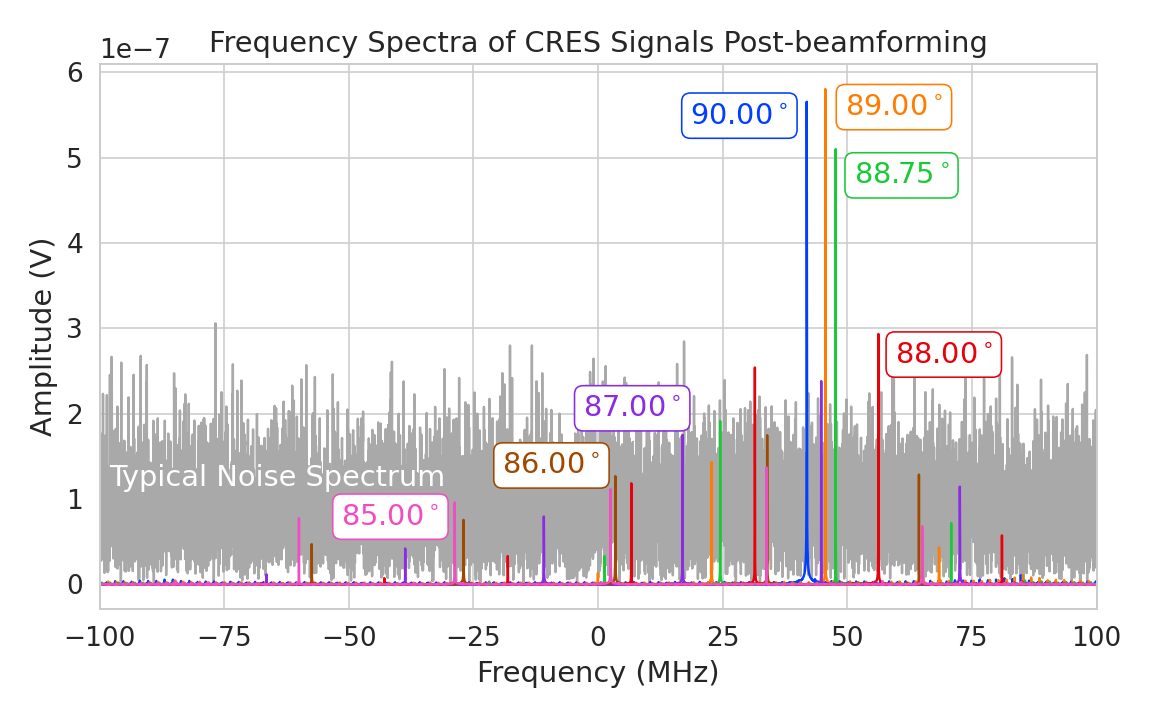
\includegraphics[width=.7\textwidth]{figs/Chapter-4/230313_cres_signal_post_bf_examples.png}
    \caption{Frequency spectra of simulated CRES signals post-beamforming. The signal of a $90^\circ$ electron consists of a single frequency component that is easy to detect with a power threshold on the frequency spectrum. This power threshold is still effective for signals with relatively large pitch angles such as $89.0^\circ$ and $88.75^\circ$, which are composed of a main carrier and a few small sidebands. Signals with smaller pitch angles, below about $88.5^\circ$, tend to be dominated by sidebands such that no single frequency component can be reliably distinguished from the noise with a power threshold.
    }
    \label{fig:signal_post_bf_example}
\end{figure}

After digital beamforming, we apply a short-time Fourier transform (STFT) to the summed time-series to obtain the frequency spectrum representation of the signals (see Figure \ref{fig:signal_post_bf_example}). From the detection perspective, the frequency representation of the CRES data is advantageous compared to the time domain, because the frequency spectra of CRES signals are well-approximated by a frequency and amplitude modulated sinusoidal whose carrier frequency increases as a linear chirp. The modulation is caused by the axial oscillation of the electron in the magnetic trap and produce frequency spectra that are well-described by a small number of frequency components. The linear chirp is caused by the energy loss due to cyclotron radiation, which results in a relatively slow increase in the frequency components of the CRES signal over time. During the standard Fourier analysis window for the FSCD of 40.96~$\mu$sec, we expect a typical CRES signal to increase in frequency by approximately 15~kHz, which is smaller than the frequency bin width given the 200~MHz sample rate. Therefore when considering a single frequency spectrum it is justifiable to neglect the effects of the linear frequency chirp. 

In the cases where the electron's pitch angle is $\gtrsim 88.5^\circ$, the majority of the signal power is contained in a single frequency component, with the remaining signal power contained in a small number of sidebands proportional to the electron's axial modulation (see Figure \ref{fig:signal_post_bf_example}). In these cases detection is relatively straight-forward by implementing a power threshold on the STFT, since the amplitude of the main signal peak is distinct from the thermal noise spectrum. However, as the pitch angle of the electron is decreased below $88.5^\circ$, the modulation index of the signal increases causing the maximum amplitude of the frequency spectrum to be comparable to typical noise fluctuations. At this point, the power threshold trigger is no longer able to distinguish between signal and noise leading to a reduction in detection efficiency. The neutrino mass sensitivity of the FSCD is directly linked to the overall detection efficiency. And, because the distribution of electron pitch angles is effectively uniformly distributed across the range of pitch angles that can be trapped, the overall detection efficiency is directly influenced by the range of pitch angles that have detectable signals. Therefore, utilizing a signal detection algorithm that can more effectively identify signals with pitch angles less than $88.5^\circ$ will improve both detection efficiency and ultimately the neutrino mass sensitivity of the FSCD and other CRES experiments. 

Modeling the detection performance of alternative signal detection algorithms for the FSCD requires that we pose the signal detection problem in a consistent manner. The approach we take is to perform a binary hypothesis test on the frequency spectra generated by the STFT. Mathematically, this is expressed as,
\begin{align}
    \mathcal{H}_0 & : y[n]=\nu[n]\\
    \mathcal{H}_1 & : y[n]=x[n]+\nu[n].
\end{align}
Where under hypothesis $\mathcal{H}_0$, the vector representing the frequency spectrum ($y[n]$) is composed of pure white Gaussian noise (WGN) represented by $\nu[n]$, and under hypothesis $\mathcal{H}_1$ the frequency spectrum is composed of a CRES signal ($x[n]$) with added WGN. The dominant source of noise in a FSCD-like experiment is expected to be thermal Nyquist-Johnson noise, which is well approximated by a WGN distribution. In order to decide between these two hypotheses we follow the standard Neyman-Pearson approach by performing a log-likelihood ratio test between the probability distributions of the signal classifier output under $\mathcal{H}_1$ and $\mathcal{H}_0$ \cite{detection_theory}. The output of the log-likelihood ratio test is called the test statistic, which is used to assign the data as belonging to the noise ($\mathcal{H}_0$) or signal ($\mathcal{H}_1$) classes by setting a decision threshold on the value of the test statistic. 

In practice, we select the decision threshold by finding the value of the test statistic that guarantees an acceptable rate of false positives and then attempt to maximize the signal detection probability under that fixed false positive rate. Because the signal classifier will be used to evaluate the spectra of $O(10^2)$ beamforming positions every 40.96~$\mu$sec, we will require the signal classifiers to operate with decision thresholds that provide false positive rates significantly smaller than 1\%. This reduces the burden placed on later stages of the CRES reconstruction chain to reject these false positives and decreases the overall likelihood of reconstructing a false event. Below, we calculate the probability distributions that allow us characterize how different detection algorithms will perform for CRES signals in an FSCD experiment.


\subsection{Signal Detection Algorithms}
\label{sec:classifiers}

\subsubsection{Power Threshold}

The power threshold detection algorithm uses the maximum amplitude of the frequency spectra  as the detection test statistic. To model the performance of this approach, consider first the case where the signal is pure WGN. For a single bin in the frequency spectrum, the probability that the amplitude falls below a specific threshold value is given by the Rayleigh cumulative distribution function (CDF),
\begin{equation}
    \mathrm{Ray}(x;\tau)=1-\exp{\left(-|x|^2/\tau\right)},
\end{equation}
where the complex amplitude of the frequency bin is $x$, and $\tau$ is the WGN variance. Because the noise samples for each frequency bin are independent and identically distributed (IID), the probability that every bin in the frequency spectrum falls below the threshold is the joint CDF formed by the product of each individual frequency bin CDF,
\begin{equation}
    F_0(x;\tau, N_\mathrm{bin})=\mathrm{Ray}(x;\tau)^{N_\textrm{bin}}.
    \label{eq:fft_spectrum_cdf0}
\end{equation}
The PDF for the power threshold classifier can then be obtained by differentiating the CDF.

\begin{figure}[htbp]
    \centering
    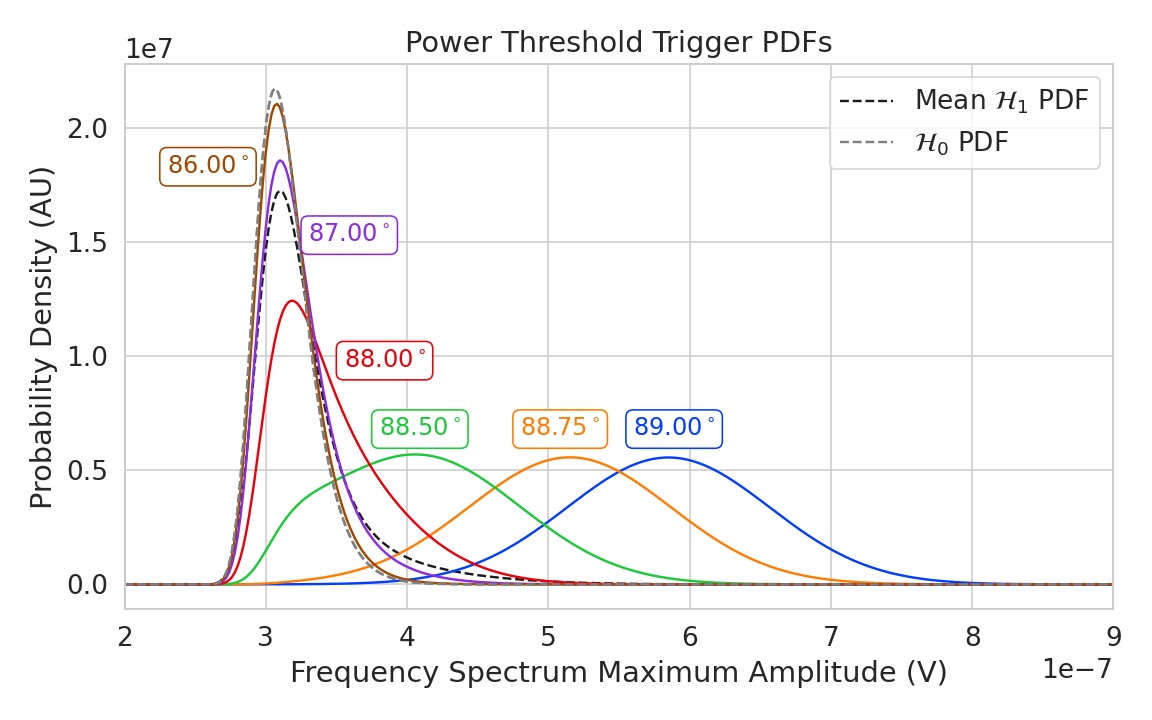
\includegraphics[width=0.7\textwidth]{figs/Chapter-4/230313_fft_power_threshold_pdf_by_pitch.png}
    \caption{PDFs of the power threshold test statistic for CRES signals with various pitch angles as well as the PDF for the noise-only signal case. The average PDF computed for pitch angles ranging from $85.5$ to $88.5^\circ$ is also shown. As the pitch angle is decreased the signal PDF converges towards the noise PDF which indicates that the power threshold trigger is unable to distiguish between small pitch angle signals and noise. }
    \label{fig:fft_pdf}
\end{figure}

The probability distribution for the power threshold classifier under $\mathcal{H}_1$ is formed in a similar way, but the frequency bins that contain signal must be treated separately. For a frequency bin that contains both signal and noise we can describe the probability that the amplitude of the bin will fall below our threshold using the Rician CDF,
\begin{equation}
    \mathrm{Rice}(x;\tau, \nu)=1-Q_1\left(\frac{|\nu|}{\sqrt{2\tau}},\frac{|x|}{\sqrt{2\tau}}\right),
\end{equation}
where the parameter $|\nu|$ defines the noise-free amplitude of the signal and $Q_1$ is the Marcum Q-function. This time the CDF that describes the probability that the entire spectrum falls below the decision threshold is the product of both signal and noise CDFs,
\begin{equation}
    F_1(x;\tau, \mathbf{\nu}, N_\mathrm{bin}, N_s)=\mathrm{Ray}(x;\tau)^{N_\mathrm{bin}-N_s}\prod_{k=0}^{N_s}{\mathrm{Rice}(x;\tau, \nu_k)}.
    \label{eq:fft_spectrum_cdf1}
\end{equation}
The first half of Equation \ref{eq:fft_spectrum_cdf1} is the contribution from the bins in the frequency spectrum that contain only noise, and the second half is the product of the Rician CDFs for the frequency bins that contain signal peaks with a noise-free amplitude of $|\nu_k|$. In Figure \ref{fig:fft_pdf} we show plots of example PDFs under $\mathcal{H}_1$ and $\mathcal{H}_0$.

\subsubsection{Matched Filtering}

The shape of a CRES signal is completely determined by the initial conditions of the electron as it is emitted from beta-decay, which implies that it is possible to apply matched filtering as a signal detection algorithm. With a matched filter one uses the shape of the known signal, which is called a template, to filter the incoming data by computing the convolution between the signal and the data \cite{detection_theory}. For cases where the signal is buried in WGN, the matched filter is the optimal detector in that it achieves the maximum probability of a true detection for a fixed false positive rate. Since CRES signals have an unknown shape but are deterministic, we can apply a matched filter by using simulations to generate a large number of signal templates called a template bank, which spans the parameter space of possible signals. Then at detection time, we use the template bank to identify signals by performing the matched filter convolution for each template in an exhaustive search.

As we saw from the frequency spectra in Figure \ref{fig:signal_post_bf_example}, CRES signals are highly periodic in nature. In such cases, it is advantageous to utilize the convolution theorem to replace the matched filter convolution with an inner product in the frequency-domain. With the convolution theorem, the matched filter test statistic that describes the detection of a signal buried in WGN using a matched filter template bank is given by
\begin{equation}
    \mathcal{T}=\max_{\mathbf{h}}\left|\sum_{n=0}^{N_\mathrm{bin}}h^\dagger[n]y[n]\right|,
    \label{eq:mf_test_stat}
\end{equation}
where $h^\dagger[n]$ is the complex conjugate of the signal template. For the case when our template bank consists of only a single template it is possible to derive an exact analytical form for the PDF describing the matched filter test statistic. First, we derive PDF under the signal hypothesis, where the equation describing the matched filter test statistic, also known as the matched filter score, becomes
\begin{equation}
    \mathcal{T}=\left|\sum_{n=0}^{N_\mathrm{bin}}h^\dagger[n]y[n]\right|.
    \label{eq:mf_inner_prod_1}
\end{equation}
Each noisy frequency bin represented by $y[n]$ is the sum between value of the signal at that bin and complex WGN, which means that $y[n]$ is itself Gaussian distributed. Therefore, the value of the inner product between the template and the data is also a complex Gaussian variable; and, since the matched filter score is the magnitude of this inner product, it must follow a Rician distribution.

We can derive the equation for the Rician PDF by expressing the matched filter template $\mathbf{h}$ in terms of the corresponding simulated signal, which we write as $\mathbf{x}_h$ to distinguish from the signal in the data. Using the standard normalization and assuming uncorrelated WGN, the matched filter templates can be written as
\begin{equation}
    \mathbf{h}=\frac{\mathbf{x}_h}{\sqrt{\tau|\mathbf{x}_h|^2}}
\end{equation}
where $\tau$ is the noise variance. Inserting this into Equation \ref{eq:mf_test_stat} and expressing the data as a sum between a signal and a WGN vector yields,
\begin{equation}
    \mathcal{T}=\frac{1}{\sqrt{\tau|\mathbf{x}_h|^2}}\left|\sum_{n=1}^{N_\mathrm{bin}}{x_h[n]\left(x[n]+\nu[n]\right)}\right|.
\end{equation}
Next, we transform the expression by isolating the randomly distributed components giving
\begin{equation}
    \mathcal{T}=\frac{\left|\sum_{n=1}^{N_\mathrm{bin}}{x_h[n]x[n]}\right|}{\sqrt{\tau|\mathbf{x}_h|^2}}+\frac{1}{\sqrt{\tau|\mathbf{x}_h|^2}}\left|\sum_{n=1}^{N_\mathrm{bin}}{x_h[n]\nu[n]}\right|.
    \label{eq:appendix-eq-1}
\end{equation}
The first term of \ref{eq:appendix-eq-1} can be simplified by using the Cauchy-Schawrz inequality to express the magnitude of the inner product in terms of the magnitudes of the signal and template as well as an orthogonality constant which we call "match" ($\Gamma$). Using this we obtain,
\begin{equation}
    \mathcal{T}=|\mathbf{h}||\mathbf{x}|\Gamma+\frac{1}{\sqrt{\tau|\mathbf{x}_h|^2}}\left|\sum_{n=1}^{N_\mathrm{bin}}{x_h[n]\nu[n]}\right|.
\end{equation}
The second term is a sum of Gaussian distributed variables, which we should expect also follows a Gaussian distribution. Each of the samples $\nu[n]$ is described by
\begin{equation}
    \nu[n]\sim \mathcal{N}(0,\tau),
\end{equation}
where $\mathcal{N}(0, \tau)$ is a complex Gaussian distribution with zero mean and variance $\tau$. Therefore,
\begin{align}
    \frac{x_h[n]}{\sqrt{\tau|\mathbf{x}_h|^2}}\nu[n]&\sim\mathcal{N}\left(0,\frac{x_h[n]^2}{|\mathbf{x}_h|^2}\right),\\
    \sum_{n=1}^{N_\mathrm{bin}}{\frac{x_h[n]}{\sqrt{\tau|\mathbf{x}_h|^2}}\nu[n]}&\sim\mathcal{N}\left(0,\frac{\sum_{n=1}^{N_\mathrm{bin}}{x_h[n]^2}}{|\mathbf{x}_h|^2}\right)=\mathcal{N}(0,1),\\
    |\mathbf{h}||\mathbf{x}|\Gamma+\sum_{n=1}^{N_\mathrm{bin}}{\frac{x_h[n]}{\sqrt{\tau|\mathbf{x}_h|^2}}\nu[n]}&\sim\mathcal{N}(|\mathbf{h}||\mathbf{x}|\Gamma,1).
\end{align}
We see that $\mathcal{T}$ is magnitude of a complex variable with mean $|\mathbf{h}||\mathbf{x}|\Gamma$ and variance one. In order to simply the expression a bit further, we define the quantity $\mathcal{T}_\mathrm{ideal}=|\mathbf{h}||\mathbf{x}|\Gamma$, which we call the ideal matched filter score, because it represents the value of the matched filter inner product that we would expect if no noise was present in the signal. We can write the matched filter test statistic as the magnitude of a two-dimensional vector in the complex plane
\begin{equation}
    \mathcal{T}=|\left(\mathcal{T}_\mathrm{ideal}+n_r, n_i\right)|,
\end{equation}
where $n_r$ and $n_i$ are the real and imaginary components of the noise each with variance $1/2$, which is modeled by a Rician distribution with shape factor $\mathcal{T}_\mathrm{ideal}$. Therefore, the probability distribution of the matched filter test statistic is given by,
\begin{equation}
    P_1(x;\mathcal{T}_\mathrm{ideal})=2x\exp{\left(-\left(x^2+\mathcal{T}_\mathrm{ideal}^2\right)\right)}I_0\left(2x\mathcal{T}_\mathrm{ideal}\right),
    \label{eq:mf_pdf_1}
\end{equation}
where $I_0$ is the zeroth-order modified Bessel function.

The shape of the matched filter score distribution is controlled by the parameter $\mathcal{T}_\mathrm{ideal}$, which is effectively the value of the matched filter score if the data contained no noise. Without noise, the data vector reduces to the signal, $\mathbf{x}$, in which case Equation \ref{eq:mf_inner_prod_1} becomes the magnitude of an inner product between two vectors. We can write the magnitude of an inner product in terms of the lengths of the individual vectors and a constant that describes the degree of orthogonality between them. Applying this to Equation \ref{eq:mf_inner_prod_1}, we obtain
\begin{equation}
    \mathcal{T}_\mathrm{ideal}=\left|\mathbf{h}^\dagger\cdot\mathbf{x}\right| = \left|\mathbf{h}\right|\left|\mathbf{x}\right|\Gamma
\end{equation}
where $\Gamma$ describes the orthogonality between $\mathbf{h}$ and $\mathbf{x}$. From the point of view of matched filtering, we can interpret $\Gamma$ as describing how well the template matches the underlying signal in the data.

The matched filter score PDF under the noise hypothesis can be readily obtained from Equation \ref{eq:mf_pdf_1} by setting the value of $\mathcal{T}_\mathrm{ideal}$ to zero, since the data contains no signal in the noise case. Doing this, we obtain the Rayleigh distribution that describes the matched filter score under $\mathcal{H}_0$,
\begin{equation}
    P_0(x) = 2x\exp{\left(-x^2\right)}.
    \label{eq:mf_pdf_0}
\end{equation}


Equations \ref{eq:mf_pdf_1} and \ref{eq:mf_pdf_0} describe the behavior of the matched filter test statistic under $\mathcal{H}_0$ and $\mathcal{H}_1$ for a single template. However, defining a PDF that describes the matched filter test statistic in the case of multiple templates is in general a mathematically intractable problem, since there is no guarantee of orthogonality between matched filter templates. This leads to correlations between the matched filter scores of different templates because only one sample of noise is used to compute the matched filter scores of the template bank. In order to proceed, we need to make the simplifying assumption that we can treat the matched filter scores as IID variables, which allows to ignore correlations between templates. The overall effect of this will be an underestimate of the performance of the matched filter, since we are under counting the number of templates that could contribute a detectable score.
 
\begin{figure}[htbp]
    \centering
    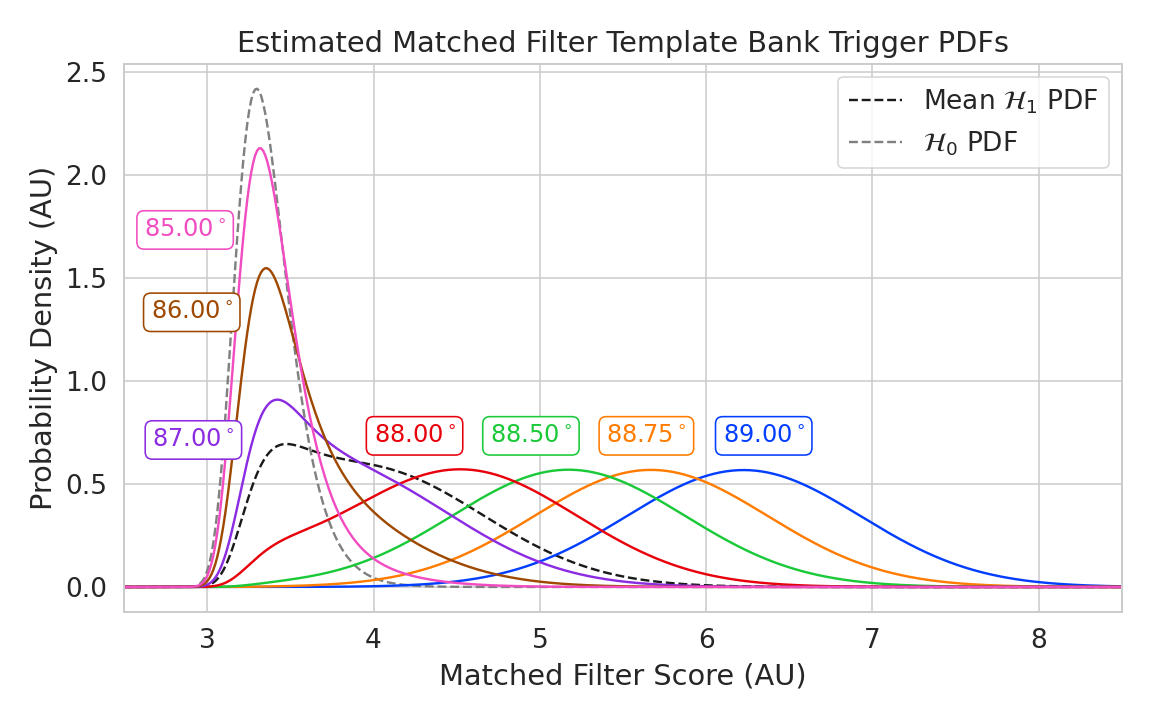
\includegraphics[width=0.7\textwidth]{figs/Chapter-4/230329_mf_pdf_by_pitch.png}
    \caption{Plots of the estimated PDFs for the matched filter template bank test statistic for CRES signals with various pitch angles as well as the estimated PDF for the noise only signal case. We assume an estimated number of templates of $10^5$ and perfect match between signal and template i.e. $\Gamma_\mathrm{best}=1$. The mean PDF includes signals ranging from $85.5-88.5^\circ$ in pitch angle. There is a much larger distinction between the signal PDFs at small pitch angle compared to the power threshold indicating a higher detection efficiency for these signals.}
    \label{fig:mf_pdf}
\end{figure}

For $\mathcal{H}_0$ we model the probability that the matched filter score falls below our threshold using the CDF obtained by integrating Equation \ref{eq:mf_pdf_0}. Because we are assuming that the matched filter scores using different templates are independent, the probability that the matched filter score for all templates falls below a threshold value is the joint CDF formed by multiplying the CDF for each template. Under $\mathcal{H}_0$ this is
\begin{equation}
    F_{0}(x) = \left(1-e^{-x^2}\right)^{N_t},
    \label{eq:mf_joint_cdf_0}
\end{equation}
where $x$ is the matched filter score threshold and $N_t$ is the number of templates. We should expect that the distribution describing the matched filter template bank maximum score depends on $N_t$, because with more templates there is a greater chance of a random match between the template and data.

For $\mathcal{H}_1$, we start by denoting the CDF of the best matching template as $F_\mathrm{best}(x;\mathcal{T}_\mathrm{best})$, and treat the matched filter scores for all other templates as negligible ($\mathcal{T}_\mathrm{ideal}\approx0$). Then we form the joint CDF by combining the distributions for all templates used during detection. Since we are exhaustively checking the matched filter scores, the number of templates checked will be a randomly distributed variable that ranges from zero to the total number of available templates. If we assume that signals are uniformly distributed across the parameter space spanned by the template bank then on average we check $(N_t-1)/2\approx N_t/2$ templates for each inference. Therefore, the estimated CDF under $\mathcal{H}_1$ is
\begin{equation}
    F_{1}(x;\mathcal{T}_\mathrm{best})=F_\mathrm{best}(x;\mathcal{T}_\mathrm{best})\left(1-e^{-x^2}\right)^{N_t/2}.
\end{equation}
In Figure \ref{fig:mf_pdf} we show plots of the estimated matched filter template bank classifier PDFs under both $\mathcal{H}_0$ and $\mathcal{H}_1$.

\subsubsection{Machine Learning}
In this paper we focus on Convolutional Neural Networks (CNN) as an example of a machine learning based signal classifier. CNNs are constructed using a series of convolutional layers, each composed of a set of filters that are convolved with the input data. The individual convolutional filters can be viewed as matched filter templates that are learned from a set of simulated data rather than being directly generated. This opens the possibility of finding a more efficient representation of the matched filter templates during the training process that can potentially reduce computational cost at inference time while still offering good classification performance. 

The machine learning approach is distinct from both the power threshold and matched filtering in that we do not attempt to manually engineer a test statistic that is computed from the data for classification. Instead, we attempt calculate the test statistic by constructing a differentiable function that maps the complex frequency series generated by the STFT to a binary classification as either signal or noise. The test statistic for the machine learning classifier can be expressed as
\begin{equation}
    \mathcal{T} = G(\mathbf{y};\mathbf{\Omega})
\end{equation}
where $\mathbf{y}$ is the noisy data vector and $G(\mathbf{y}; \mathbf{\Omega})$ is the machine learning model parameterized by the weights $\mathbf{\Omega}$. By using supervised learning on a labeled set of training signals, we can modify the function parameters to learn the mapping from the data to the likelihood of $\mathbf{y}$ belonging to either $\mathcal{H}_1$ or $\mathcal{H}_0$.

\begin{table}[h]
\centering
\caption{A summary of the CNN model layers and parameters. The output of each 1D-Convolution and Fully Connected layer is passed through a LeakyReLU activation function and re-normalized using batch normalization before being passed to the next layer in the model. The output of the final Fully Connected layer in the model is left without activation so that the model outputs can be directly passed to the Binary Cross-entropy loss function used during training. \label{tab:cnn_model_params}}
\smallskip
\begin{tabular}{|c|c|c|c|c|}
\hline
Layer&Type&Input Channels&Output Channels&Parameters\\
\hline
1 & 1D-Convolution & 2 & 15 & ($N_{\textrm{kernel}}=4$, $N_{\textrm{stride}}=1$)\\
2 & Maximum Pooling & 15 & 15 & ($N_{\textrm{kernel}}=4$, $N_{\textrm{stride}}=4$) \\
3 & 1D-Convolution & 15 & 20 & ($N_{\textrm{kernel}}=4$, $N_{\textrm{stride}}=1$)\\
4 & Maximum Pooling & 20 & 20 & ($N_{\textrm{kernel}}=4$, $N_{\textrm{stride}}=4$) \\
5 & 1D-Convolution & 20 & 25 & ($N_{\textrm{kernel}}=4$, $N_{\textrm{stride}}=1$)\\
6 & Maximum Pooling & 25 & 25 & ($N_{\textrm{kernel}}=4$, $N_{\textrm{stride}}=4$) \\
7 & Fully Connected & 3200 & 512 & NA \\
8 & Fully Connected & 512 & 64 & NA \\
9 & Fully Connected & 64 & 2 & NA \\
\hline
\end{tabular}
\end{table}

The CNN architecture used for this work is summarized by Table \ref{tab:cnn_model_params}. No strategic hyper-parameter optimization approach was implemented beyond the manual testing of different CNN architecture variations, so this particular model is best viewed as a proof-of-concept rather than a rigorously optimized design. Numerous model variations were tested, some with significantly more layers and convolutions filters per layer, as well as others that were even smaller than the architecture in Table \ref{tab:cnn_model_params}. Ultimately, the model architecture choice was driven by the motivation to find the minimal model whose classification performance was still comparable to the larger CNN's tested, because of the importance of minimizing computational cost in real-time applications. It is possible that more sophisticated machine learning models could improve upon the classification results achieved here, but we leave this investigation for future work.

\subsection{Methods}
\label{sec:method}


\subsubsection{Data Generation}
\label{sec:datasets}
To test the triggering performance of the classifiers, simulated CRES signals were generated using the Locust simulations package \cite{p8locustpaper, nb_thesis} developed by the Project 8 collaboration. Locust uses the separately developed Kassiopeia package to calculate the magnetic fields produced by a user defined set of current carrying coils along with any specified background magnetic fields, resulting in a magnetic trap. Next, Kassiopeia calculates the trajectory of an electron in this magnetic field starting from a set of user specified initial conditions. The Locust software then uses the electron trajectories from Kassiopeia to calculate the resulting electromagnetic fields using the Li\'{e}nard-Wiechert equations, and determine the voltages generated in the antenna array with the antenna transfer function. Locust then simulates the down-conversion, filtering, and digitization steps resulting in the simulated CRES signals for an electron.

The shape of the received CRES signal is determined by the initial kinematic parameters, including the starting position of the electron, the starting kinetic energy of the electron, and the pitch angle. For the studies performed here we constrain ourselves to a single initial electron position located at $(x,y,z)=(5, 0, 0)$~mm, and using this starting position we generate two datasets by varying the initial kinetic energy and the starting pitch angle. The first dataset consists of a two-dimensional square grid of kinetic energy and pitch angle spanning an energy range from 18575-18580~eV with a spacing of 0.1~eV, and pitch angles from $85.5$-$88.5^\circ$ with a spacing of $0.001^\circ$, resulting in 153051 signals with a unique energy-pitch angle combination. This dataset is intended to represent a matched filter template bank. The second dataset was generated by randomly sampling uniform probability distributions covering the same parameter space to produce approximately 50000 signals randomly parameterized in energy and pitch angle. This dataset provides the training and test data for the machine learning approach, and acts as a representative sample of signals to evaluate the performance of the matched filter template bank.

Each signal was simulated for a duration of $40.96$~$\mu$s, which is equivalent to 8192 samples at the FSCD digitization rate, and begins at time $t=0$~s for all simulations. This duration represents a single frequency spectrum generated by the STFT. The output of the Locust simulation is a matrix of array snapshots with size given by the number of channels times the event length ($N_\textrm{ch}\times N_\textrm{sample}$), which we pre-process using the digital beamforming summation and STFT described in Section \ref{sec:bf-and-stft}. The $\nabla B$-drift correction uses the exact value of $\omega_{\nabla B}$, obtained from the Kassiopeia simulation of that electron. In practice, an average value for $\omega_{\nabla B}$ could be used, because there is limited variation in drift frequency across this parameter space.

\subsubsection{Template Number and Match Estimation}
The estimated PDF for the matched filter template bank depends on the score of the best matching template or equivalently the match of the best template ($\Gamma_\mathrm{best}$) as well as the number of templates. One expects that with a higher number of templates the average value of $\Gamma_\mathrm{best}$ will increase, however, there is a point of diminishing returns at which more templates will not significantly increase match, but will still increase the likelihood of false positives. Therefore, it is desirable to use the minimum number of templates that provide an acceptable mean value of $\Gamma_\mathrm{best}$.
\begin{figure}[htbp]
    \centering
    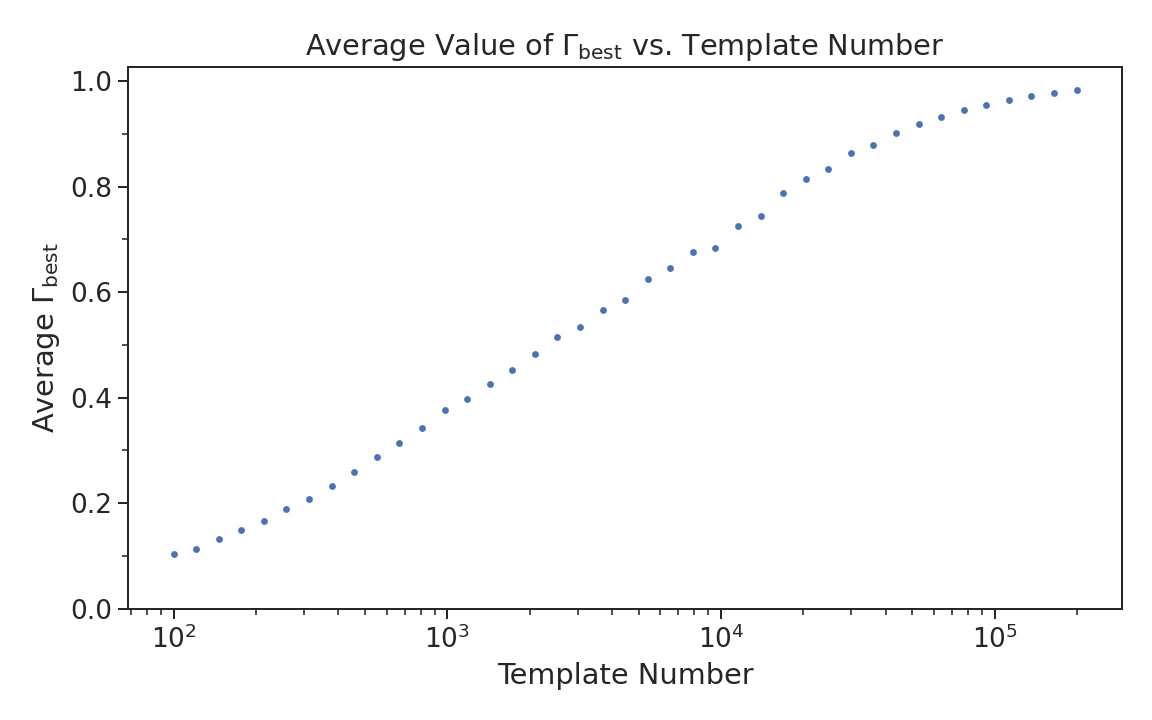
\includegraphics[width=0.6\textwidth]{figs/Chapter-4/230426_mean_match_vs_templates.png}
    \caption{The mean match of the matched filter template bank to a test set of randomly parameterized signals as a function of the number or density of templates. The parameter space includes pitch angles from $85.5-88.5^\circ$ and energies from $18575-18580$~eV.}
    \label{fig:match_vs_template_number}
\end{figure}

To quantify the relationship between match and template number, we calculated the mean match of the random dataset to a selection of templates obtained from the regularly spaced dataset. The results are shown in Figure \ref{fig:match_vs_template_number}, where we find that the average value of $\Gamma_\mathrm{best}$ is an exponential function of the number of templates. From this plot we select the desired value of mean match at which we would like to evaluate the matched filter PDF and can infer the required number of templates. 

\subsubsection{CNN Training and Data Augmentation}
To prepare the data for training the model, we split the random dataset in half to create distinct training and test datasets. Additionally, a randomly selected 20\% of the training data is isolated for use as a validation set during the training loop. The size of the training, validation, and test datasets are then tripled by appending two additional copies of the data to increase the sample size of the dataset after data augmentation. The data is loaded with no noise, which is added to each data batch during the training phase by generating a new noise sample from a complex WGN distribution. In order to ensure an even split between signal and noise data we append to the noise-free signals an equal number of empty signals composed of all zeros. Therefore, as the data is randomly shuffled during training, on average an equal number of empty signals will be included with the training signals. After adding the sample of WGN to the data batch, the empty signals represent the noise-only data that the model must distinguish from signal data. 

As the training signals are loaded we apply a unique random phase shift as the first form of data augmentation. Since the data is generated using the same initial axial position and cyclotron orbit phase, the randomization is an attempt to prevent overtraining on these features. During each training epoch the data is randomly shuffled and split into batches of 2500 signals. Each batch of signals is then circularly shifted by a random number of frequency bins to simulate a kinetic energy shift from $-75$ to $20$~eV to simulate a training dataset with a larger energy range. Next, a sample of complex WGN, consistent with the expected 10~K Nyquist-Johnson noise  expected for the FSCD, is generated and added to the signal, which prevents overtraining on noise features. As a final step, the data is renormalized by the standard deviation of the noise so that the range of values in the data is close to $[-1,1]$, which helps ensure well-behaved back-propagation.

\begin{figure}[htbp]
    \centering
    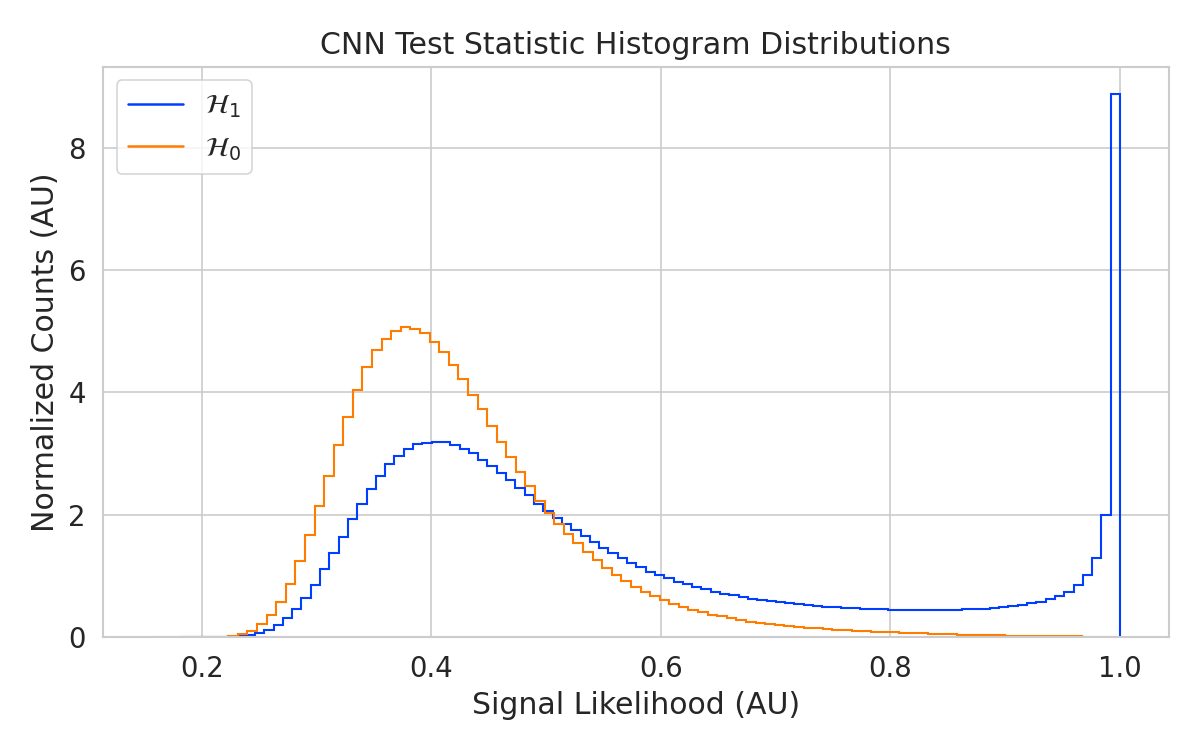
\includegraphics[width=0.6\textwidth]{figs/Chapter-4/230324_cnn_test_stat_hist.png}
    \caption{Histograms of the trained CNN model output from the test dataset. The blue histogram shows the model outputs for signal data. The oddly shaped peak near the end is the result of the softmax function mapping the long tail of the raw output distribution to the range $[0,1]$. }
    \label{fig:cnn_histogram}
\end{figure}

The Binary Cross-entropy loss function is used to compute the loss for each batch of data and the model weights are updated using the ADAM optimizer with a learning rate of $5\times10^{-3}$. After each training epoch, the loss and classification accuracy of the validation dataset are computed to monitor for overtraining. It was noticed that the relatively high noise power and the fact that a new sample of noise was used for each batch together provided a strong form of regularization, since no evidence of over-training was observed even after several thousand epochs. Typically, the loss and classification accuracy of the model converged after a few hundred training epochs, but the training loop was extended to 3000 epochs to attempt to achieve the best possible performance. The training procedure generally took about 24~hrs using a single NVIDIA V100 GPU \cite{v100}.

After training the model, we use it to classifying the test dataset and generate histograms of the model outputs for both classes of data. The data augmentation procedure for the evaluation of the test data mirrors the training procedure without the validation split. Since a random circular shift and a new sample of WGN is added to each batch, the testing evaluation loop is run for 100 epochs to get a representative sample of noise and circular shifts. The model outputs for each batch are passed through a softmax activation and then combined into histograms, which we show in Figure \ref{fig:cnn_histogram}.

\subsection{Results and Discussion}
\label{sec:results}


\subsubsection{Trigger Classification Performance}

\begin{figure}[htbp]
    \centering
    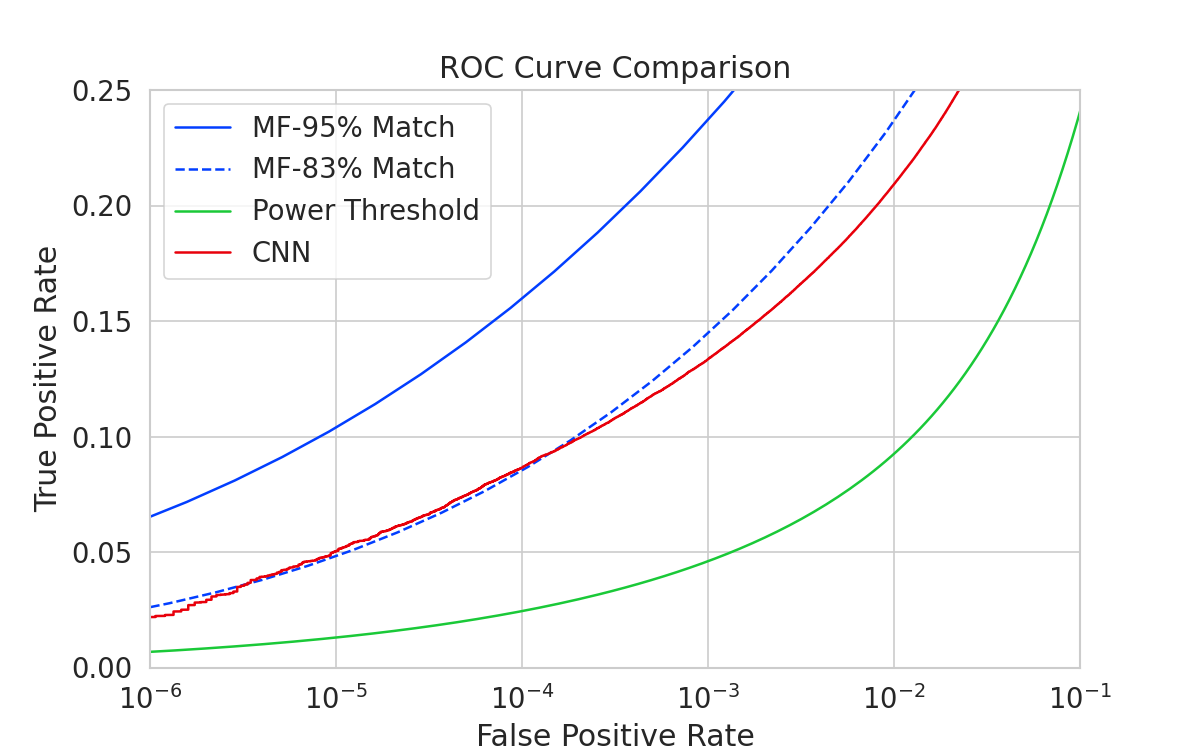
\includegraphics[width=0.7\textwidth]{figs/Chapter-4/230327_nn_roc_vs_mf_vs_fft.png}
    \caption{ROC curves describing the detection efficiency or true positive rates for the three signal classification algorithms examined in this paper.
    }
    \label{fig:roc_compare}
\end{figure}
Using the matched filter and power threshold CDFs, along with the classification results from the CNN, we compare detection performance by computing receiver operating characteristic (ROC) curves. Specifically, we compare the detection performance averaged over the full signal parameter space in order to get a measure of the overall detection efficiency achieved by each algorithm. For the power threshold and matched filter algorithms, we obtain the mean ROC curve by taking the average over all signals in the regularly spaced dataset. In the case of the matched filter, we examine two cases using different numbers of templates, which have different values of mean match. The ROC curve describing the CNN is obtained by forming a histogram of the network outputs for each class of signal and from this computing the estimated CDFs and ROC curve. In Figure \ref{fig:roc_compare}, we show the ROC curves obtained for each of the detection algorithms, visualized in terms of true positive rate and false positive rate.

The true positive rate of a signal classifier is equivalent to its detection efficiency, and we see that for the population of signals with pitch angles $<88.5^\circ$ the power threshold has a consistently lower detection efficiency than the CNN and the matched filter. This result could have been predicted from the visualization of signal spectra in Figure \ref{fig:signal_post_bf_example}, where we see that there is no way to distinguish between a noise peak and a signal peak with high confidence at small pitch angles. The CNN offers a significant and consistent increase in detection efficiency over the power threshold approach, with the relative improvement in detection efficiency increasing as the false positive rate decreases. If we compare the CNN to the matched filter, we see that the performance of the tested network is roughly equivalent to a matched filter detector with an average match of about 83\%, which uses approximately 20000 matched filter templates. The overall best detection efficiency is achieved by the matched filter classifier if a large enough template bank is used. We show in the plot the ROC curve for a matched filter template bank with 95\% average match, which is achieved with approximately $100000$ templates. Since the matched filter is known to be statistically optimal for detecting a known signal in WGN, it is somewhat expected that this algorithm has the highest detection efficiency.

A potentially impactful difference between the matched filter and CNN algorithms is that the CNN relies upon convolutions as its fundamental calculation mechanism, whereas our implementation of a matched filter utilizes an inner product. Since convolution is a translation invariant operation, the detection performance of CNN can be extended to a wider range of CRES event kinetic energies with less cost than the matched filter, a feature that we exploited during the CNN training by including circular translations of the CRES frequency spectra in the training loop. Increasing the range of kinetic energies detectable by a matched filter requires a proportional increase in the number of templates, which directly translates into increased computational and hardware costs. From a practical perspective, the detection algorithm is always limited by the available computational hardware, so estimating the relative costs is a key factor in determining their feasibility. Below we perform a more detailed analysis of the relative costs of each of the detection algorithms.


\subsubsection{Computational Cost and Hardware Requirements}
\label{sec:dis-comp-cost}


In the process of investigating triggering approaches for an antenna array CRES experiment, we have uncovered a strong tension between detection efficiency and computational resources. To relate the computational cost estimates to actual costs, we compare the theoretical amount of computer hardware required to implement the signal classifiers for real-time detection in an FSCD experiment. To do this we shall utilize order of magnitude estimates of the theoretical peak performance values for currently available Graphics Processing Units (GPUs) as a metric. This approach will underestimate the amount of required hardware, since it is unlikely that any CRES detection algorithm could reach the theoretical peak performance of the hardware. 

Of the three detection algorithms tested, the power threshold classifier is the least expensive. It requires that we check whether the amplitude of each frequency bin in the STFT is below or above our decision threshold. The STFT combined with digital beamforming produces $N_\mathrm{bin}N_\mathrm{b}$ frequency bins that must be checked every $N_\mathrm{bin}/f_\mathrm{s}$ seconds. This requires approximately $O(10^{10})$ FLOPS to check in real-time. Current generations of GPUs have peak theoretical performances in the range of $O(10^{13})-O(10^{14})$~FLOPS \cite{h100}, dependent on the required floating-point precision of the computation. Therefore, the entire computational needs of a real-time triggering system using a power threshold classifier, including digital beamforming and generation of the STFT, could be met by a single high-end GPU or a small number of less powerful GPUs. Since triggering is only one step of the full real-time signal reconstruction approach, limiting the computational cost of this stage is ideal. However, we have seen that the power threshold classifier does not provided sufficient detection efficiency across the entire range of possible signals, which is the primary motivation for exploring more complicated triggering solutions. 

As discussed, the computational cost of the matched filter approach requires counting the number of templates that must be checked for each frequency spectra produced by the STFT. Computing the matched filter scores requires $O(N_\mathrm{b}N_\mathrm{t}N_\mathrm{bin})$ operations, since for each of the $N_\mathrm{b}$ beamforming positions we must multiply $N_\mathrm{t}$ templates with a data vector that has length $N_\mathrm{bin}$. The time within which we must perform this calculation is equal to $N_\mathrm{bin}/f_\mathrm{s}$ to keep up with the data generation rate. To cover the 5~eV kinetic energy range spanned by the template bank, we saw that $10^4$ to $10^5$ templates are required in order to match or exceed the detection efficiency of the CNN. If the number of templates scales linearly with then kinetic energy range of interest as expected, then we would require $10^5$ to $10^6$ matched filter templates with this more realistic range of energies. Considering this, the estimated computational cost of the matched filter is between $O(10^{15})$ to $O(10^{16})$~FLOPS, which is $O(10^2)$ to $O(10^3)$ high-end GPUs.

Lastly, we have the CNN classifier. To estimate the computational cost we simply sum the number of convolutions and matrix multiplications specified by the network architecture shown in Table \ref{tab:cnn_model_params}. Each convolutional layer consists of $N_\mathrm{in}N_\mathrm{out}N_\mathrm{kernel}L_\mathrm{input}$ floating-point operations, where $N_\mathrm{in}$ is the number of input channels, $N_\mathrm{out}$ is the number of output channels, $N_\mathrm{kernel}$ is the size of the convolutional kernel, and $L_\mathrm{input}$ is the length of the input vector, and the fully connected layers each contribute $N_\mathrm{in}N_\mathrm{out}$ operations. Summing all the neural network layers we estimate that the CNN would require $O(10^6)$ floating point operations for each frequency spectra; therefore, the total computation cost of the CNN trigger is this cost times the number of beamforming positions per the data acquisition time, which is $O(10^{13})$~FLOPS or $O(10^0)$ GPUs.

Compared with the matched filter approach the CNN requires $O(100)$ to $O(1000)$ fewer GPUs to implement, dependent on the exact number of templates used in the template bank. The 100~eV kinetic energy range is motivated by the application of these detection algorithms to an FSCD-like neutrino mass measurement experiment. However, if a significantly larger range of kinetic energies is required, a CNN may be the preferred detection approach despite the lower average detection efficiency due to computational cost considerations. The low estimated computational cost of the CNN is directly related to the small network size.


Additional experiments with larger CNNs, generated by increasing the depth and width of the neural network, and we observed that these changes provided minimal ($\lesssim 1\%$) improvement in the classification accuracy of the model. A potential reason for this could be the sparse nature of the signals in the frequency domain and the low SNR which makes for a challenging dataset to learn from. Future work could investigate modifications to the neural network architecture such as sparse convolutions, which may improve the classification accuracy of the model or further reduce the computational costs of this approach. Alternatively, more complicated CNN architectures such as a ResNet \cite{resnet} or VGG model \cite{vgg} may provide improved classification performance over a basic CNN. An additional promising area of investigation are recurrent neural networks, which may be able to exploit the time-ordered features of the STFT for more accurate signal detection if the electron signals last for multiple Fourier transform windows.

Our estimate of the computational cost of the matched filter is somewhat naive if we notice that the majority of the values that make up a CRES frequency spectra are zero (see Figure \ref{fig:signal_post_bf_example}). Therefore, the majority of operations in the matched filter inner product are unnecessary, and we could instead evaluate the matched filter inner product using only the $\lesssim10$ frequency peaks that make up CRES signal. This optimization reduces the number of operations required to check each template by a factor of $O(100)$ to $O(1000)$, which brings the estimated computational cost of the matched filter in line with the CNN. Although this level of sparsity results in a multiplication with very low arithmetic complexity, the resulting sparse matched filter algorithm is still likely to be constrained by memory access speed rather than compute speed. Ultimately, the comparison of the relative computational and hardware costs between the matched filter and CNN will depend on the efficiency of the software implementation and hardware support for neural network and sparse matrix calculations.


\subsection{Conclusion}
\label{sec:conclusion}

Increasing the detection efficiency and overall event rate of the CRES technique represents a key developmental path towards new scientific results and broader applications of the CRES technique. It is what motivates both the antenna array detection approach and the development of real-time signal reconstruction algorithms. We have demonstrated that significant gains in the detection efficiency of the CRES technique are achievable by utilizing triggering algorithms that account for the specific shape of CRES signals in the detector. These algorithms emphasize the need for accurate and fast methods for CRES simulation, since they directly contribute to the success of matched filter methods by providing a way to generate expected signal templates and also serve as a source of training data for machine learning approaches. % This is particularly true for antenna array approaches to CRES measurement due to the low signal power.

The improvements in detection efficiency offered by these alternative approaches to triggering are crucial to the success of efforts to develop scalable technologies for CRES measurement, since they provide a significant increase in the detectable parameter space of CRES events, which allows for a better utilization of the larger detection volume. While we have focused on the real-time detection of CRES signals from antenna arrays, these same signal classifiers could be used in CRES experiments utilizing a different detector technologies, since the same principles of signal detection will apply. For example, previous CRES measurements by the Project 8 collaboration that utilized a waveguide gas cell, could have improved their detection efficiency by employing a matched filter or neural network classifier to identify trapped electrons with pitch angles that are too small to be detected by the power threshold approach. Furthermore, alternative CRES detector technologies such as resonant cavities \cite{p8snowmass2022} could also see similar improvements in detection efficiency, which is of crucial importance to future efforts by the Project 8 collaboration to utilize CRES to measure the neutrino mass.


